%\documentclass[a4paper,9pt,landscape]{article}
\documentclass[a4paper,11pt]{article}
\usepackage{amsfonts}
\usepackage[cm]{fullpage}
\usepackage{pdflscape}
\usepackage{tikz}
\usepackage{siunitx}
\usepackage{amssymb}
\usepackage{upgreek}
\usepackage{multicol}
\usepackage{bm}
\usepackage{url}
\usepackage{amsmath}
\usepackage{mdframed}
\usepackage{listings}
\usepackage{nopageno}
\usepackage{csquotes}
\newcommand{\nn}{\nonumber}
\newcommand{\Ranb}{{\mathsf{Ra}}}
\newcommand{\Renb}{{\mathsf{Re}}}
\newcommand{\Nunb}{{\mathsf{Nu}}}
\newcommand{\Prnb}{{\mathsf{Pr}}}
\newcommand{\Penb}{{\mathsf{Pe}}}
\newcommand{\Dinb}{{\mathsf{Di}}}
\newcommand{\bN}{{\mathcal{N}}}
\newcommand{\bM}{{\mathcal{M}}}
\newcommand{\A}{{\mathbb{A}}}
\newcommand{\K}{{\mathbb{K}}}
\newcommand{\J}{{\mathbb{J}}}
\newcommand{\G}{{\mathbb{G}}}
\newcommand{\Z}{{\mathbb{Z}}}
\newcommand{\C}{{\mathbb{C}}}
\newcommand{\W}{{\mathbb{W}}}
\newcommand{\R}{{\mathbb{R}}}
\newcommand{\M}{{\mathbb{M}}}
\newcommand{\N}{{\mathbb{N}}}
\newcommand{\Q}{{\mathbb{Q}}}
\newcommand{\LLL}{{\mathbb{L}}}
\newcommand{\SSS}{{\mathbb{S}}}
\newcommand{\captionfont}{\tiny}

%\usepackage{biblatex} %Imports biblatex package
%\addbibresource{biblio_geosciences.bib,biblio_lou} %Import the bibliography file

\newcommand{\BoxT}{{\color{teal} \boxplus}}
\newcommand{\BoxB}{{\color{brown} \boxplus}}
\newcommand{\BoxV}{{\color{violet} \boxplus}}
\newcommand{\BoxR}{{\color{red} \boxplus}}
\usetikzlibrary{arrows, arrows.meta}
\lstset{ 
  language=Python,
  backgroundcolor=\color{white},   % choose the background color; you must add \usepackage{xcolor}; should come as last argument
  basicstyle=\footnotesize,        % the size of the fonts that are used for the code
  breakatwhitespace=false,         % sets if automatic breaks should only happen at whitespace
  breaklines=true,                 % sets automatic line breaking
  captionpos=b,                    % sets the caption-position to bottom
  frame=single,                    % adds a frame around the code
  keepspaces=true,                 % keeps spaces in text, useful for keeping indentation of code 
  keywordstyle=\color{blue},       % keyword style
}

%\renewcommand{\baselinestretch}{2} 
\renewcommand{\baselinestretch}{1.1} 

%%%%%%%%%%%%%%%%%%%%%%%%%%%%%%%%%%%%%%%%%%%%%%%%%%%%%%%%%%%%%%%%%%%%%%%
\begin{document}

\tableofcontents

%------------------------------------------------------------------------------
\section{Non-dimensionalisation of the Navier-Stokes equations}\label{ss:nondim}
\begin{flushright} {\tiny {\color{gray} physics.tex}} \end{flushright}



{\color{red} write it all for dev stress instead of deviatoric strain rate!}

- Where does the term anelastic come from ?

- What do we really gain from the TALA, EBA and such ? 

- What makes for a good choice of nondimensionalisation variables ?

- check zhyu96b

%______________________________________________
\subsection{Approach \# 1 - isothermal flow}
%We start from the following form of the momentum conservation equation: 
%\[
%\frac{\partial \vec\upnu}{\partial t} + (\vec\upnu \cdot \vec\nabla)\vec\upnu 
%=
%-\frac{1}{\rho}\vec\nabla p + \nu \Delta \vec \upnu + \vec g
%\]
%where $\nu$ is the kinematic viscosity. \index{general}{Kinematic Viscosity}

We define (see for instance \cite{maqs06} (2006)) four reference 
quantities which are relevant for geodynamics\footnote{Note that in the paper 
the authors conflate $\rho$ and $\tilde{\rho}$ which prevents them from non-dimensionalising all terms as we do here.}:
\begin{itemize}
\item a reference viscosity value $\underline{\eta}=10^{20}~\si{\pascal\second}$
\item a reference mass density $\underline{\rho}=1000~\si{\kg\per\cubic\metre}$
\item a reference time $\underline{t}=1\text{Myr}\simeq 3.15\cdot 10^{13}~\si{\second}$
\item a reference length $\underline{l}=1000~\si{\metre}$
\item a reference gravity $\underline{g}=9.81~\si{\metre\per\square\second}$
\end{itemize}
It follows that a reference pressure can be obtained:
\[
\underline{p}=\underline{\rho} \underline{g} \underline{l} = 9.81\cdot 10^6~\si{\pascal}
\]
Note that there is unfortunately no natural selection for the pressure scale. 
We could also have used $\underline{p}=\underline{\rho}\underline{\upnu}^2$ 
where dynamic effects are dominant i.e. high velocity flows,
or $\underline{p}=\underline{\eta}\underline{\upnu}/\underline{l}$ 
where viscous effects are dominant i.e. creeping flows (which 
is the case in geodynamics).
The definition of a reference velocity is more straightforward: $\underline{\upnu} = \frac{\underline{l}}{\underline{t}}$. %= 1~\si{\mm\per\year}

We define dimensionless variables through:
\[
{\color{teal}x} = \frac{x}{\underline{l}}
\qquad
{\color{teal}y} = \frac{y}{\underline{l}}
\qquad
{\color{teal}z} = \frac{z}{\underline{l}}
\qquad
{\color{teal}\vec\upnu'} = \frac{\vec\upnu}{\underline{\upnu}}
\qquad
{\color{teal}t} = \frac{t}{\underline{t}}
\qquad
{\color{teal} \eta} = \frac{\eta}{\underline{\eta}}
\qquad
{\color{teal} g} =\frac{g}{\underline{g}}
\qquad
{\color{teal} \rho} =\frac{\rho}{\underline{\rho}}
\qquad
{\color{teal} p} = \frac{p}{\underline{p}}=\frac{p}{\underline{\rho}\underline{g} \underline{l}}
\]
where the {\color{teal}teal} color indicates dimensionless values.
Consequently, time and space derivatives will be rescaled as follows:
${\color{teal} \vec\nabla} = \underline{l}\; \vec\nabla$ and ${\color{teal} \partial_t} = \underline{t}\; \partial_t$.
Using this scaling relations the momentum conservation equation becomes:
\[
\rho \left( 
\frac{ \underline{l}}{\underline{t}^2} {\color{teal} \frac{\partial \vec\upnu}{\partial t}}
+ \frac{ \underline{l}}{\underline{t}^2} {\color{teal} (\vec\upnu \cdot\vec\nabla) \vec\upnu}  \right)
=- \underline{\rho} \underline{g} {\color{teal} \vec\nabla p}
+ \frac{\underline{\eta}}{\underline{l}\underline{t}} 
{\color{teal} \vec\nabla \cdot \eta (\vec\nabla \vec \upnu + \vec\nabla \vec \upnu ^T)}
+ \underline{\rho} \underline{g}  {\color{teal} \rho \vec{g}}
\]
We divide each side by $\underline{\rho} $:
\[
{\color{teal} \rho} \left( 
\frac{ \underline{l}}{\underline{t}^2} {\color{teal} \frac{\partial \vec\upnu}{\partial t}}
+ \frac{ \underline{l}}{\underline{t}^2} {\color{teal} (\vec\upnu \cdot\vec\nabla) \vec\upnu}  \right)
=-  \underline{g} {\color{teal} \vec\nabla p}
+ \frac{\underline{\eta}}{\underline{l}\underline{t} \underline{\rho}} 
{\color{teal} \vec\nabla \cdot \eta (\vec\nabla \vec \upnu + \vec\nabla \vec \upnu ^T)}
+ \underline{g}   {\color{teal} \rho \vec{g}}
\]
and now multiply each side by $\underline{t}^2 /\underline{l}$:
\[
{\color{teal} \rho} \left( 
{\color{teal} \frac{\partial \vec\upnu}{\partial t}}
+  {\color{teal} (\vec\upnu \cdot\vec\nabla) \vec\upnu}  \right)
=- \frac{\underline{t}^2 \underline{g}   }{\underline{l}} {\color{teal} \vec\nabla p}
+ \frac{\underline{\eta}\underline{t} }{\underline{\rho} \underline{l}^2 } 
{\color{teal} \vec\nabla \cdot \eta (\vec\nabla \vec \upnu + \vec\nabla \vec \upnu ^T)}
+ \frac {\underline{g} \underline{t}^2 }{ \underline{l} }  {\color{teal} \rho \vec{g}}
\]
One can recognise in this equation the Reynolds\footnote{\url{https://en.wikipedia.org/wiki/Reynolds_number}} 
and Froude\footnote{\url{https://en.wikipedia.org/wiki/Froude_number}} 
non-dimensional numbers (the ratio between the inertial and viscous forces, and the 
ratio between buoyancy and inertial forces respectively). 
\[
Re = \frac{\underline{\rho} \underline{l}^2}{\underline{\eta} \underline{t} }
\qquad
Fr= \frac{\underline{l}}{\underline{g}\underline{t}^2 }
\]




We can then write:
\[
\boxed{
{\color{teal}\rho} \left(
{\color{teal} \frac{\partial \vec\upnu}{\partial t}}
+
{\color{teal} (\vec\upnu \cdot\vec\nabla) \vec\upnu}  \right)
=
- \frac{1}{Fr} {\color{teal} \vec\nabla p}
+
\frac{1}{Re}
{\color{teal} \vec\nabla \cdot \eta (\vec\nabla \vec \upnu + \vec\nabla \vec \upnu ^T)}
+ \frac{1}{Fr} {\color{teal} \vec{g}}
}
\]
or 
\[
\boxed{
Re \; {\color{teal}\rho} \left(
{\color{teal} \frac{\partial \vec\upnu}{\partial t}}
+
{\color{teal} (\vec\upnu \cdot\vec\nabla) \vec\upnu}  \right)
=
- \frac{Re}{Fr} {\color{teal} \vec\nabla p}
+
{\color{teal} \vec\nabla \cdot \eta (\vec\nabla \vec \upnu + \vec\nabla \vec \upnu ^T)}
+ \frac{Re}{Fr} {\color{teal} \vec{g}}
}
\]



In our case, given the definitions taken above, we have:
\[
Re \simeq 3.174 \cdot 10^{-24}
\qquad
Fr \simeq 1.027 \cdot 10^{-25}
\qquad
\frac{Re}{Fr} = 
\frac{\underline{\rho} \underline{l}^2}{\underline{\eta} \underline{t} }
\frac{\underline{g}\underline{t}^2 }{\underline{l}}
=\frac{\underline{\rho} \underline{g}\underline{t} \underline{l}}{\underline{\eta}  }
=\simeq 30.5
\]
so we conclude that inertial forces in the Earth's mantle
are small compared to viscous forces
and that the inertial terms can be dropped from the momentum 
equation (thereby yielding the dimensionless Stokes equations):
\[
{\color{teal} \vec\nabla \cdot \eta (\vec\nabla \vec \upnu + \vec\nabla \vec \upnu ^T)}
- \frac{Re}{Fr} {\color{teal} \vec\nabla p}
+ \frac{Re}{Fr}  {\color{teal} \vec{g} }
=0
\]



\subsection{Approach \# 2 - Temperature dependent \label{ss:dimeqs2}}


Let us now consider a box heated from below and cooled from above. 
We define 4 {\color{violet} fundamental reference} quantities:
\begin{itemize}
\item a length ${\color{violet} \underline{L}}$ (\si{\metre})
\item a temperature ${\color{violet} \underline{T}}$ (\si{\kelvin})
\item a viscosity ${\color{violet} \underline{\eta}}$ (\si{\pascal\second}=\si{\kg\per\meter\per\second})
\item a thermal diffusion coefficient ${\color{violet} \underline{\kappa}}$ (\si{\square\metre\per\second}), 
\end{itemize}
They collectively contain the set of {\color{violet}fundamental dimensions} (length, time, mass and temperature) so we express any other physical quantity as a function of these and
establish a set of {\color{purple}secondary reference} quantities:
\begin{itemize}
\item a reference time (\si{\second}):
${\color{purple}\underline{t}} = 
{\color{violet} \underline{L}}^2 / {\color{violet} \underline{\kappa}}$ (aka the diffusion time)

\item a reference velocity (\si{\meter\per\second}):
${\color{purple}\underline{\upnu}} = {\color{violet} \underline{L}} / {\color{purple}\underline{t}} 
= {\color{violet} \underline{\kappa}}/{\color{violet} \underline{L}}$

\item a reference acceleration (\si{\meter\per\second^2}):
${\color{purple}\underline{g}} = {\color{purple}\underline{\upnu}} / {\color{purple}\underline{t}} = {\color{violet} \underline{\kappa}}^2/{\color{violet} \underline{L}}^3$

\item a reference strain rate (\si{\per\second}):
${\color{purple}\dot{\underline{\varepsilon}}} = {\color{purple}\underline{t}}^{-1} = {\color{violet} \underline{\kappa}} / {\color{violet} \underline{L}}^2$

\item a reference pressure/stress (\si{\pascal}):
${\color{purple}\underline{p}} = {\color{purple}\underline{\tau}}= {\color{violet}\underline{\eta}} {\color{purple}\dot{\underline{\varepsilon}}} = {\color{violet}\underline{\eta}} {\color{purple}\underline{t}}^{-1} = 
{\color{violet} \underline{\eta}} {\color{violet} \underline{\kappa}} / 
{\color{violet} \underline{L}}^2$

\item a reference mass (\si{\kg}):
${\color{purple}\underline{M}} 
= {\color{violet}\underline{\eta}} {\color{violet}\underline{L}} {\color{purple}\underline{t}}
= {\color{violet}\underline{\eta}} {\color{violet}\underline{L}} {\color{violet}\underline{L}}^2 / {\color{violet}\underline{\kappa}}
= {\color{violet} \underline{\eta}} {\color{violet} \underline{L}}^3/ {\color{violet} \underline{\kappa}}$

\item a reference density (\si{\kg\per\cubic\meter}):
${\color{purple}\underline{\rho}}
= {\color{purple}\underline{M}}/{\color{violet}\underline{L}}^3
= {\color{violet}\underline{\eta}} {\color{violet}\underline{L}}^3/ {\color{violet}\underline{\kappa}} / {\color{violet}\underline{L}}^3
= {\color{violet} \underline{\eta}} / {\color{violet} \underline{\kappa}}$

\item a reference energy (\si{\joule}):
${\color{purple}\underline{E}}
= {\color{purple}\underline{M}} \cdot {\color{purple}\underline{\upnu}}^2
= {\color{violet}\underline{\eta}} {\color{violet}\underline{L}}^3/ {\color{violet}\underline{\kappa}}  
\cdot {\color{violet}\underline{\kappa}}^2/{\color{violet}\underline{L}}^2
= {\color{violet} \underline{\eta} \underline{L}}   {\color{violet} \underline{\kappa}} 
$

\item a reference heat conductivity (\si{\watt\per\meter\per\kelvin}):
${\color{purple}\underline{k}}= {\color{purple}\underline{E}}\cdot {\color{purple}\underline{t}}^{-1} \cdot 
{\color{violet}\underline{L}}^{-1} \cdot {\color{violet}\underline{T}}^{-1}
= 
{\color{violet}\underline{\eta}} {\color{violet}\underline{L}} {\color{violet}\underline{\kappa}}
\cdot 
{\color{violet}\underline{L}}^{-2}  {\color{violet}\underline{\kappa}}
\cdot
{\color{violet}\underline{L}}^{-1} 
\cdot
{\color{violet}\underline{T}}^{-1}
=
{\color{violet} \underline{\eta}} {\color{violet} \underline{L}}^{-2} 
{\color{violet} \underline{\kappa}^2 \underline{T}}^{-1}
$



\item a reference heat capacity (\si{\joule\per\kg\per\kelvin}):
${\color{purple}\underline{C}_p}={\color{purple}\underline{E}} {\color{purple}\underline{M}}^{-1} 
{\color{violet}\underline{T}}^{-1} = 
{\color{violet} \underline{\eta} \underline{L}}   {\color{violet} \underline{\kappa}} 
\cdot 
({\color{violet} \underline{\eta}} {\color{violet} \underline{L}}^3/ {\color{violet} \underline{\kappa}})^{-1} \cdot {\color{violet} \underline{T}}^{-1}
= 
{\color{violet} \underline{\kappa}}^2 {\color{violet}  \underline{L}}^{-2}
{\color{violet} \underline{T}}^{-1}
$

\item a reference heat production coefficient (\si{\watt\per\kg}):
${\color{purple}\underline{H}}= {\color{purple}\underline{E}} 
\cdot {\color{purple}\underline{t}}^{-1} \cdot {\color{purple}\underline{M}}^{-1} 
= {\color{violet} \underline{\eta} \underline{L}}   {\color{violet} \underline{\kappa}} 
\cdot
({\color{violet} \underline{L}}^2 / {\color{violet} \underline{\kappa}})^{-1} 
\cdot
({\color{violet} \underline{\eta}} {\color{violet} \underline{L}}^3/ 
{\color{violet} \underline{\kappa}})^{-1}
= {\color{violet} \underline{\kappa}}^3 {\color{violet} \underline{L}}^{-4}
$

\item a reference thermal expansion (\si{\per\kelvin}): 
${\color{purple} \underline{\alpha}} = {\color{violet} \underline{T}}^{-1}$

%\item a reference heat flux\footnote{Units: \si{\watt\per\square\meter}, or %\si{\kg\per\cubic\second}} 
%$\underline{q} = \underline{\eta} \underline{L} \underline{t}^{-2}$
\end{itemize}




We define {\color{teal}dimensionless} quantities as follows:
\begin{equation}
{\color{teal}x} = \frac{x}{\color{violet}\underline{L}}
\quad
{\color{teal}\vec\upnu} = \frac{\vec\upnu}{\color{purple} \underline{\upnu}}
\quad
{\color{teal}t} = \frac{t}{\color{purple}\underline{t}}
\quad
{\color{teal} \eta} = \frac{\eta}{\color{violet} \underline{\eta}}
\quad
{\color{teal} g} =\frac{g}{\color{purple}\underline{g}}
\quad
{\color{teal} k} = \frac{k}{\color{purple}\underline{k}}
\quad
{\color{teal} C_p} = \frac{C_p}{\color{purple}\underline{C}_p}
\quad
{\color{teal} \rho} =\frac{\rho}{\color{purple}\underline{\rho}}
\end{equation}

\begin{equation}
{\color{teal} H} = \frac{H}{\color{purple}\underline{H}}
\quad
{\color{teal} \vec\nabla} = {\color{violet}\underline{L}}\; \vec\nabla
\quad
{\color{teal} \partial_t} = {\color{purple}\underline{t}}\; \partial_t 
\quad
{\color{teal} T} = \frac{T}{\color{violet}\underline{T}}
\quad
{\color{teal} \dot{\varepsilon}} = \dot{\varepsilon} \; {\color{purple}\underline{t}}
\quad
{\color{teal} \alpha} = \frac{\alpha}{\color{purple} \underline{\alpha}}
\label{eq:physics_adimrels}
\end{equation}

\subsubsection{Momentum equation} 

We start from the standard momentum conservation equation of the Navier-Stokes 
equation\footnote{\url{https://en.wikipedia.org/wiki/Navier-Stokes_equations}}
\[
\rho \frac{D \vec\upnu}{D t}
= -\vec\nabla p + \vec\nabla \cdot (2 \eta \dot{\bm\varepsilon}^d)
+ \rho \vec{g} 
\]
where $D/Dt$ is the material derivative, and we assume that the density is 
only temperature-dependent (see for example the Boussinesq approximation) so that
\[
\rho \frac{D \vec\upnu}{D t}
= -\vec\nabla p + \vec\nabla \cdot (2 \eta \dot{\bm\varepsilon}^d)
+ \rho_0(1-\alpha T) \vec{g} 
\]
and remove the hydrostatic pressure (although we keep using $p$ for simplicity, $p$ is now the dynamic pressure):
\[
\rho \frac{D \vec\upnu}{D t}
=
-\vec\nabla p + \vec\nabla \cdot (2 \eta \dot{\bm\varepsilon}^d)
- \rho_0\alpha T \vec{g} 
\]
We divide this equation by 
$\underline{p}=\underline{\eta}\dot{\underline{\varepsilon}}$:
\[
\frac{1}{\underline{\eta}\dot{\underline{\varepsilon}}} \rho
\frac{D \vec\upnu}{D t} 
=
-\vec\nabla {\color{teal}p} + \vec\nabla \cdot 2 \frac{\eta}{\underline{\eta}} \frac{\dot{\bm\varepsilon}^d}{\dot{\underline{\varepsilon}}}
- \frac{\rho_0\alpha T \vec{g}}{\underline{\eta} \dot{\underline{\varepsilon}}} 
\]
Let us call $\vec{e}$ the positive vertical vector ($\vec{e}_z$ in Cartesian coordinates, $\vec{e}_r$ in spherical coordinates), then 
$\vec{g} = -g_0 \vec{e}$ and we can write 
(using $\dot{\underline{\varepsilon}}=\underline{\kappa}/\underline{L}^2$
in the buoyancy term only)
\[
\frac{1}{\underline{\eta}\dot{\underline{\varepsilon}}}
(\underline{\rho}{\color{teal}\rho})\frac{D(\underline{\upnu} {\color{teal}\vec\upnu})}{D t}
=
-\vec\nabla {\color{teal}p} + \vec\nabla \cdot 2 {\color{teal} \eta} {\color{teal} \dot{\bm\varepsilon}}
+ \frac{\rho_0\alpha T g_0 }{\underline{\eta} (\underline{\kappa}/ \underline{L}^2)} \vec{e}
\]
Dividing by $\underline{L}^{-1}$ (i.e. multiplying by $\underline{L}$) yields
\[
\frac{\underline{\upnu} \underline{\rho} \underline{L}}{\underline{\eta}\dot{\varepsilon}_{ref}  }
{\color{teal}\rho} \frac{{\color{teal} D \vec\upnu}}{ \underline{t} {\color{teal} D t}}
=
-{\color{teal} \vec\nabla} {\color{teal}p} + {\color{teal} \vec\nabla} \cdot 2 {\color{teal} \eta} {\color{teal} \dot{\bm\varepsilon}}
+ \frac{\rho_0\alpha ({\color{teal}T}\underline{T}) g_0 \underline{L}^3}{\underline{\eta} \underline{\kappa}} \vec{e}
\]
and finally (using $\underline{\upnu}=\underline{L}/\underline{t}$
and 
$\dot{\underline{\varepsilon}}=\underline{\kappa}/\underline{L}^2$ again) 
\[
\frac{\underline{\rho} \underline{\kappa}}{\underline{\eta}}
{\color{teal}\rho} \frac{{\color{teal} D \vec\upnu}}{\color{teal} D t}
=
-{\color{teal} \vec\nabla} {\color{teal}p} + {\color{teal} \vec\nabla} \cdot 2 {\color{teal} \eta} {\color{teal} \dot{\bm\varepsilon}}
+ \frac{\rho_0\alpha \underline{T} g_0 \underline{L}^3}{\underline{\eta} \underline{\kappa}} {\color{teal} T} \vec{e}
\]
In the context of a system with a temperature difference $\Delta T$ 
between the bottom and top boundaries separated by a distance $H$, one would then take $\underline{T} = \Delta T$ 
and $\underline{L}=H$ so that the equation becomes:
\[
\underbrace{\frac{\underline{\rho} \underline{\kappa}}{\underline{\eta}}}_{\Prnb^{-1}}
{\color{teal}\rho} \frac{{\color{teal} D \vec\upnu}}{\color{teal} D t}
=
-{\color{teal} \vec\nabla} {\color{teal}p} + {\color{teal} \vec\nabla} \cdot 2 {\color{teal} \eta} {\color{teal} \dot{\bm\varepsilon}}
+ \underbrace{\frac{\rho_0\alpha \Delta T g_0 H^3}{\underline{\eta} \underline{\kappa}} }_{\Ranb} {\color{teal} T}\vec{e}
\]
and we obviously recover the classical definition of the Rayleigh number.
The dimensionless equation then becomes:
\begin{mdframed}[backgroundcolor=blue!5]
\[
\frac{1}{\Prnb}
{\color{teal}\rho} \frac{{\color{teal} D \vec\upnu}}{\color{teal} D t}
=
-{\color{teal} \vec\nabla} {\color{teal}p} + {\color{teal} \vec\nabla} \cdot 2 {\color{teal} \eta} {\color{teal} \dot{\bm\varepsilon}}
+ \Ranb {\color{teal} T}\vec{e}
\]
\end{mdframed}


On the left side of the equation we recognize the (inverse of the) Prandlt number $\Prnb=\frac{\eta}{\rho \kappa}$. 
We can estimate the dimensionless number before the inertial term for Earth
geodynamics:
\[
\Prnb \simeq \frac{10^{20-23}}{3000 \cdot 10^{-6}} >> 10^{23}
\]
Its inverse is then extremely small and this is why we neglect the inertial terms
in mantle modelling.

Let us now revisit this all again by assuming that the density is now 
given by 
\[
\rho(T,p)= \rho_0( 1 -\alpha (T-T_0) + K_T^{-1} p )
\]
where $T_0$ is a reference temperature and $K_T$ is the isothermal bulk modulus.
We have the rhs of the momentum equation :
\begin{eqnarray}
\rho \vec{g} 
&=& \rho_0( 1 -\alpha (T-T_0) + K_T^{-1} p ) \vec{g} \nn\\
&=& \rho_0( 1 -\alpha (T-T_0) ) \vec{g} +  \rho_0 K_T^{-1} p  \vec{g} \nn\\
\end{eqnarray}
The first term of the rhs will yield the $\Ranb {\color{teal}T}$ term, so we now turn to the second one.

{\color{red} FINISH}

%Note that if the fluid is isoviscous, one can then set $\underline{\eta}=\eta=\eta_0$ and then ${\color{teal}\eta}=1$ 
%and then 
%\[
%-{\color{teal} \vec\nabla} {\color{teal}p} + {\color{teal} \vec\nabla} \cdot 2  {\color{teal} \dot{\bm\varepsilon}}
%+ \Ranb {\color{teal} T} \vec{e}= \vec{0}
%\]
\subsubsection{Continuity equation} 

Turning now to the continuity equation $\vec\nabla \cdot (\rho \vec\upnu) = 0$,
it is trivial to show that  
${\color{teal} \vec\nabla } \cdot  {\color{teal} \rho \vec\upnu} = 0$.

\subsubsection{Energy equation} 

Looking now at the Extended Boussinesq Approximation (EBA), we have the following energy equation:
\[
\rho C_p \left(\frac{\partial T}{\partial t} + \vec \upnu\cdot\vec\nabla T\right)
- \vec\nabla\cdot k\vec\nabla T 
= \rho H + {\bm \tau} : \vec\nabla \vec\upnu
+\alpha T  \vec\upnu \cdot \vec\nabla p 
\]

{\color{red} which rho and p ??}


Using the definitions of the fundamental and secondary reference quantities, as well as 
Eq.\eqref{eq:physics_adimrels} we can write
\[
{\color{teal} \rho} {\color{purple} \underline{\rho}}
{\color{teal} C_p} {\color{purple} \underline{C_p}} {\color{violet} \underline{T}}
\left(\frac{\partial {\color{teal} T} }{\partial t} + 
{\color{purple} \underline{\upnu}} {\color{teal} \vec\upnu}
\cdot\vec\nabla {\color{teal} T}  \right)
- {\color{violet} \underline{T}} {\color{purple} \underline{k}} 
\vec\nabla\cdot {\color{teal} k} \vec\nabla {\color{teal}T} 
= {\color{teal} \rho} {\color{purple} \underline{\rho}}
{\color{teal} H} {\color{purple} \underline{H}}
+ {\color{purple} \underline{p}} {\color{purple} \underline{\upnu}}
{\color{teal} {\bm \tau}}:
\vec\nabla   {\color{teal} \vec\upnu}
+
{\color{purple} \underline{\alpha}}
{\color{purple} \underline{p}}
{\color{violet} \underline{T}}
{\color{purple} \underline{\upnu}}
{\color{teal} \alpha} 
{\color{teal} T} 
{\color{teal} \vec\upnu} \cdot \vec\nabla {\color{teal} p} 
\]
We keep going with the space and time derivatives.
We have
\begin{eqnarray}
{\color{purple} \underline{\upnu}} {\color{teal} \vec\upnu} \cdot\vec\nabla {\color{teal} T}  
&=&
{\color{purple} \underline{\upnu}} {\color{teal} \vec\upnu} \cdot 
\frac{1}{\color{violet} \underline{L}}{\color{teal}\vec\nabla }{\color{teal} T}  
=\frac{ {\color{violet} \underline{\kappa}}}{ {\color{violet} \underline{L}}^2 }
 {\color{teal} \vec\upnu} \cdot {\color{teal}\vec\nabla }{\color{teal} T}  
\nn\\
\frac{\partial {\color{teal} T} }{\partial t} 
&=& \frac{1}{ \color{purple} \underline{t}} {\color{teal} \frac{\partial T}{\partial t} }
= \frac{ {\color{violet} \underline{\kappa}}}{ {\color{violet} \underline{L}}^2 }
{\color{teal} \frac{\partial T}{\partial t} }
\nn\\
\vec\nabla \cdot {\color{teal} k} \vec\nabla {\color{teal}T} 
&=&
\frac{1}{\color{violet} \underline{L}^2}
{\color{teal}\vec\nabla } \cdot {\color{teal} k \vec\nabla T} 
\nn
\\
{\color{teal} {\bm \tau}}: \vec\nabla   {\color{teal} \vec\upnu} &=& 
\frac{1}{\color{violet} \underline{L}}
{\color{teal} {\bm \tau}}: {\color{teal}\vec\nabla \vec\upnu   }
\nn\\
{\color{teal} \vec\upnu} \cdot \vec\nabla {\color{teal} p} 
&=&
\frac{1}{\color{violet} \underline{L}}
{\color{teal} \vec\upnu \cdot \vec\nabla  p} 
\end{eqnarray}
Putting it all together:
\[
{\color{purple} \underline{\rho}} 
{\color{purple} \underline{C_p}} 
{\color{violet} \underline{T}}
\frac{ \color{violet} \underline{\kappa}  }{\color{violet} \underline{L}^2}
{\color{teal} \rho C_p}  
\left({\color{teal} \frac{\partial T}{\partial t} }
+{\color{teal} \vec\upnu} \cdot {\color{teal}\vec\nabla }{\color{teal} T}  
 \right)
- {\color{violet} \underline{T}} {\color{purple} \underline{k}} 
\frac{1}{\color{violet} \underline{L}^2}
{\color{teal}\vec\nabla } \cdot {\color{teal} k \vec\nabla T} 
= 
{\color{purple} \underline{\rho}} {\color{purple} \underline{H}}
{\color{teal} \rho} {\color{teal} H} 
+
{\color{purple} \underline{p}} {\color{purple} \underline{\upnu}} \frac{1}{\color{violet} \underline{L}}
{\color{teal} {\bm \tau}}: {\color{teal}\vec\nabla \vec\upnu   }
+
{\color{purple} \underline{\alpha}}
{\color{purple} \underline{p}}
{\color{violet} \underline{T}}
{\color{purple} \underline{\upnu}}
\frac{1}{\color{violet} \underline{L}}
{\color{teal} \alpha} 
{\color{teal} T} 
{\color{teal} \vec\upnu \cdot \vec\nabla  p} 
\]

We have 
\begin{eqnarray}
{\color{purple} \underline{\rho}} 
{\color{purple} \underline{C_p}} 
{\color{violet} \underline{T}}
\frac{ \color{violet} \underline{\kappa}  }{\color{violet} \underline{L}^2}
&=& {\color{violet} \underline{\eta}} / {\color{violet} \underline{\kappa}}
\cdot 
{\color{violet} \underline{\kappa}}^2 {\color{violet}  \underline{L}}^{-2}
{\color{violet} \underline{T}}^{-1}
\cdot
{\color{violet} \underline{T}}
\frac{ \color{violet} \underline{\kappa}  }{\color{violet} \underline{L}^2} 
=
{\color{violet} \underline{\eta}}^1
{\color{violet} \underline{\kappa}}^2
{\color{violet} \underline{L}}^{-4}
{\color{violet} \underline{T}}^{0}
\nn\\
\nn\\
%%%%%%%%%%%%%%%%%%%%%%%%%%%%%%%%%%%%%%%%
{\color{violet} \underline{T}} {\color{purple} \underline{k}} 
\frac{1}{\color{violet} \underline{L}^2}
&=& 
{\color{violet} \underline{T}} 
\cdot
{\color{violet} \underline{\eta}} {\color{violet} \underline{L}}^{-2} 
{\color{violet} \underline{\kappa}^2 \underline{T}}^{-1}
\cdot 
\frac{1}{\color{violet} \underline{L}^2}
=
{\color{violet} \underline{\eta}}^1
{\color{violet} \underline{\kappa}}^2
{\color{violet} \underline{L}}^{-4}
{\color{violet} \underline{T}}^{0}
\nn\\
%%%%%%%%%%%%%%%%%%%%%%%%%%%%%%%%%%%%%%%%
{\color{purple} \underline{\rho}} {\color{purple} \underline{H}}
&=& 
{\color{violet} \underline{\eta}}  / {\color{violet} \underline{\kappa}}
\cdot 
{\color{violet} \underline{\kappa}}^3 {\color{violet} \underline{L}}^{-4}
=
{\color{violet} \underline{\eta}}^1
{\color{violet} \underline{\kappa}}^2
{\color{violet} \underline{L}}^{-4}
{\color{violet} \underline{T}}^0
\nn\\
%%%%%%%%%%%%%%%%%%%%%%%%%%%%%%%%%%%%%%%%
{\color{purple} \underline{p}} {\color{purple} \underline{\upnu}} 
\frac{1}{\color{violet} \underline{L}}
&=& 
{\color{violet} \underline{\eta}}   {\color{violet} \underline{\kappa}} / {\color{violet} \underline{L}}^2
{\color{violet} \underline{\kappa}} / {\color{violet} \underline{L}}
\cdot
\frac{1}{\color{violet} \underline{L}}
=
{\color{violet} \underline{\eta}}^1
{\color{violet} \underline{\kappa}}^2
{\color{violet} \underline{L}}^{-4}
{\color{violet} \underline{T}}^0
\nn\\
%%%%%%%%%%%%%%%%%%%%%%%%%%%%%%%%%%%%%%%%
{\color{purple} \underline{\alpha}}
{\color{purple} \underline{p}}
{\color{violet} \underline{T}}
{\color{purple} \underline{\upnu}}
\frac{1}{\color{violet} \underline{L}}
&=&
{\color{violet} \underline{T}}^{-1}
\cdot
{\color{violet} \underline{\eta}} {\color{violet} \underline{\kappa}} / {\color{violet} \underline{L}}^2
\cdot
{\color{violet} \underline{T}}
\cdot
{\color{violet} \underline{\kappa}}/{\color{violet} \underline{L}}
\frac{1}{\color{violet} \underline{L}}
=
{\color{violet} \underline{\eta}}^1
{\color{violet} \underline{\kappa}}^2
{\color{violet} \underline{L}}^{-4}
{\color{violet} \underline{T}}^0
\end{eqnarray}

since all four coefficients are equal we 
can then write
\[
{\color{teal} \rho C_p}  
\left({\color{teal} \frac{\partial T}{\partial t} }
+{\color{teal} \vec\upnu} \cdot {\color{teal}\vec\nabla }{\color{teal} T}  
 \right)
- {\color{teal}\vec\nabla } \cdot {\color{teal} k \vec\nabla T} 
= 
{\color{teal} \rho} {\color{teal} H} 
+
{\color{teal} {\bm \tau}}: {\color{teal}\vec\nabla \vec\upnu   }
+
{\color{teal} \alpha} 
{\color{teal} T} 
{\color{teal} \vec\upnu \cdot \vec\nabla  p} 
\]


\newpage
%%%%%%%%%%%%%%%%%%%%%%%%%%%%%%%%%%%%%%%%%%%%%%%%%%%%%%%%%%%%%%%%%%%%%%%%%%%%%%%
\section{Exploring the literature}

%%%%%%%%%%%%%%%%%%%%%%%%%%%%%%%%%%%%%%%%%%%%%%%%%%%%%%%%%%%%%%%%%%%%%%%%%%%%%%%
\subsection{Solheim \& Peltier (1990)}

This article comes early in the literature and is referred to by many subsequent 
published studies looking at/using compressible formulations. We read \cite{sope90}:

\begin{displayquote}  {\color{darkgray}
The main focus of the present paper will be to describe the basic mathematical
and numerical structure of our new axially symmetric anelastic model and to
present an overview of some of the main results that we have obtained with it to
date.}
\end{displayquote}

\begin{center}
\fbox{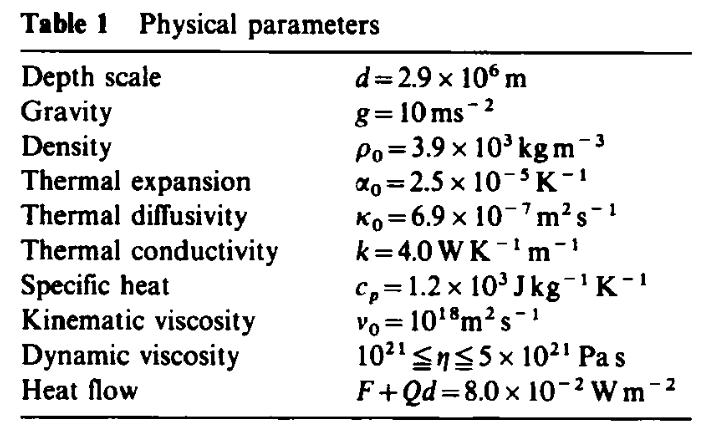
\includegraphics[width=7cm]{images/sope_01}}\cite{sope90}
\end{center}

\begin{center}
\fbox{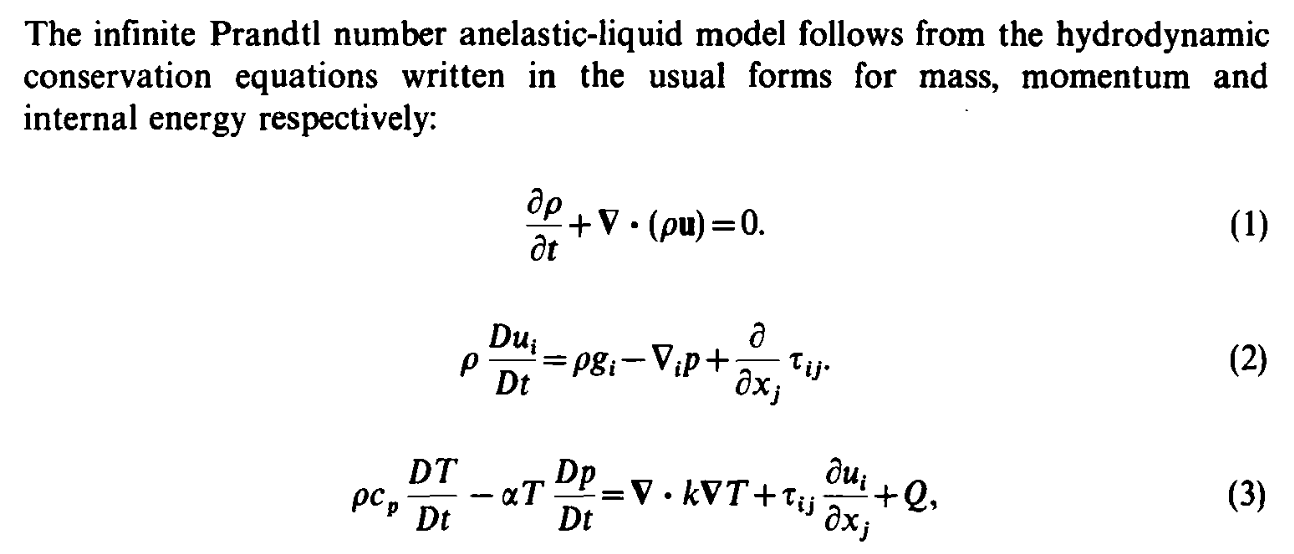
\includegraphics[width=14cm]{images/sope_02}}\cite{sope90}\\
{\tiny I agree with these, standard conservation equations.}
\end{center}

\begin{center}
\fbox{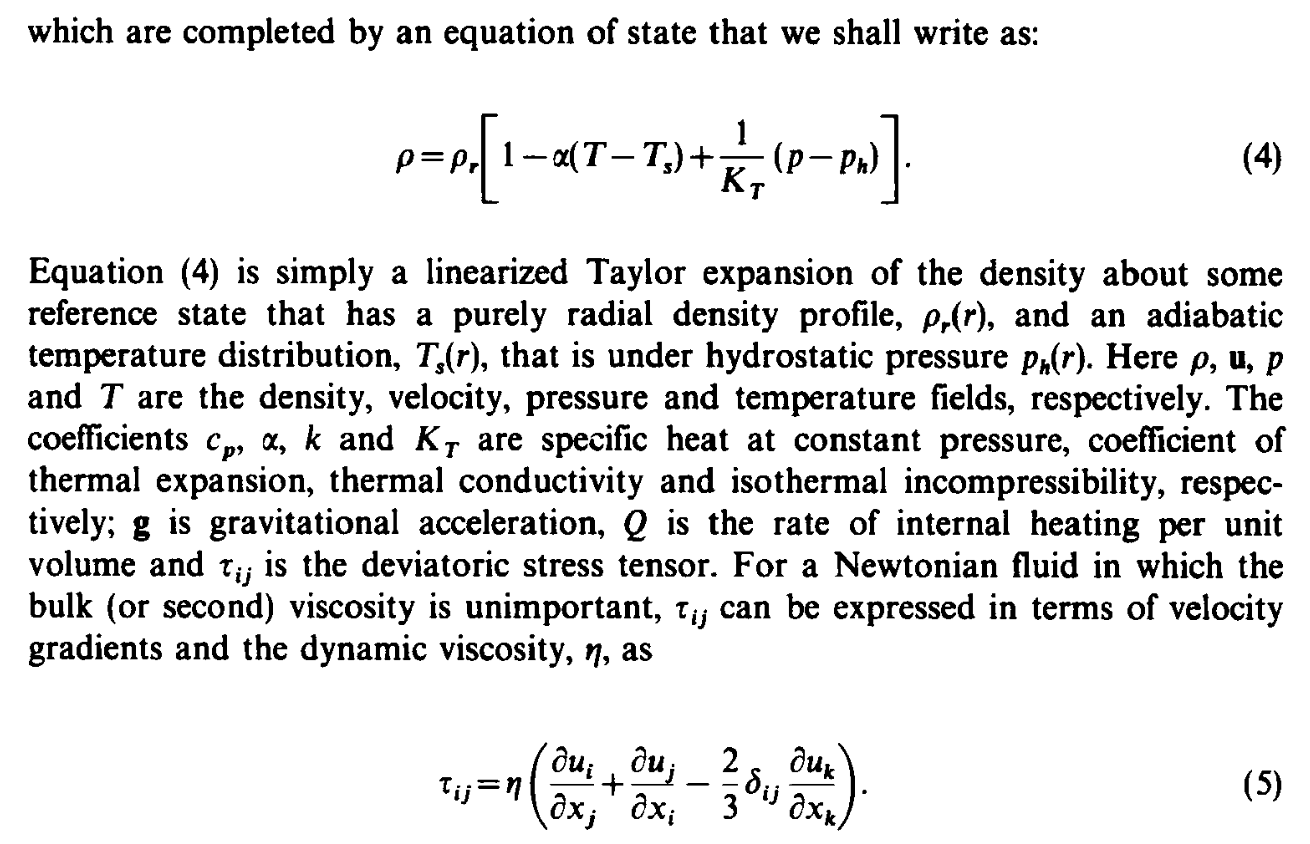
\includegraphics[width=14cm]{images/sope_03}}\cite{sope90}
\end{center}


\begin{center}
\fbox{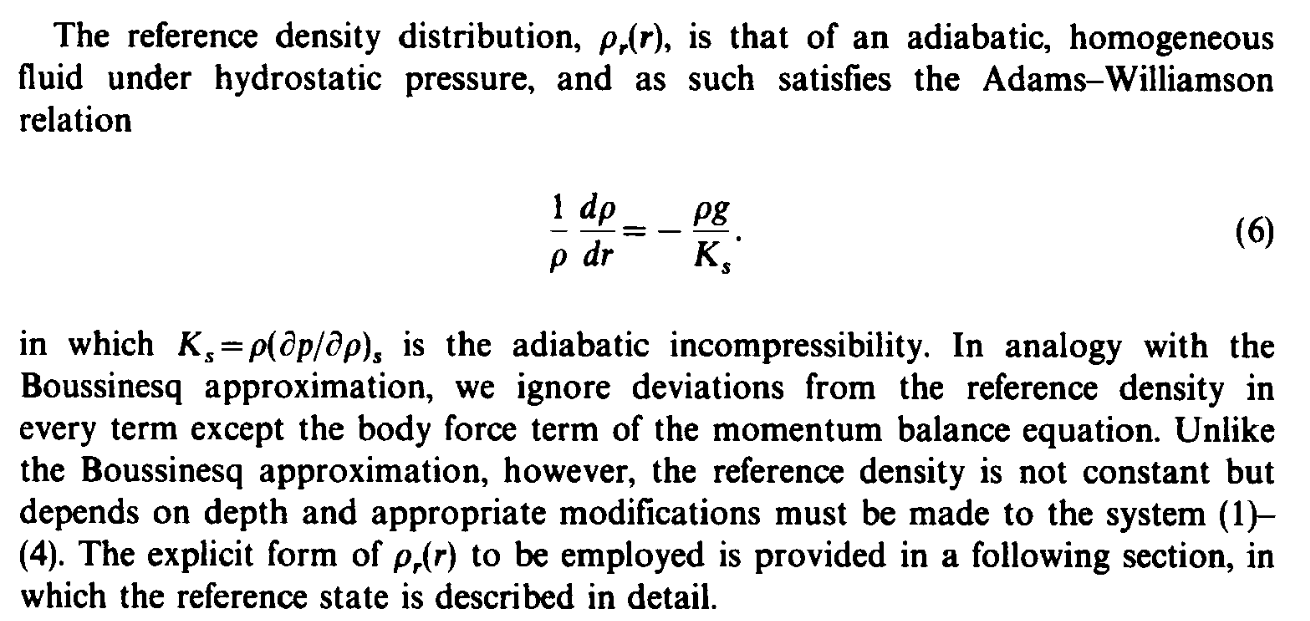
\includegraphics[width=14cm]{images/sope_04}}\cite{sope90}
\end{center}

The authors then explain why the $\partial \rho/\partial t$ term can be 
neglected:
\begin{center}
\fbox{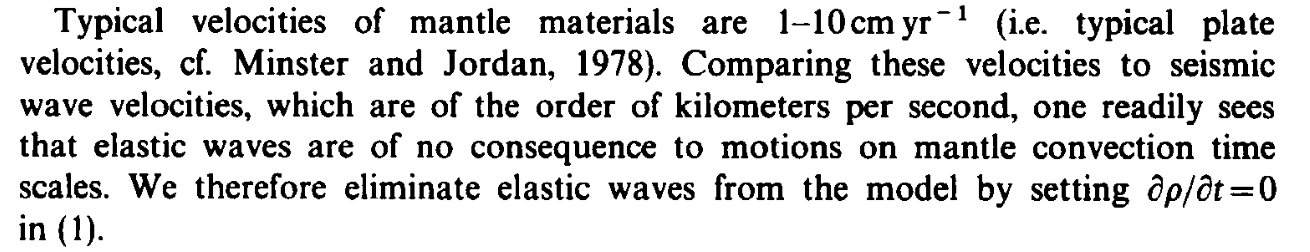
\includegraphics[width=14cm]{images/sope_05}}\cite{sope90}
\end{center}

They then present the formulation for the radial pressure (In the equations the density $\rho$ should be the radial density):
\begin{center}
\fbox{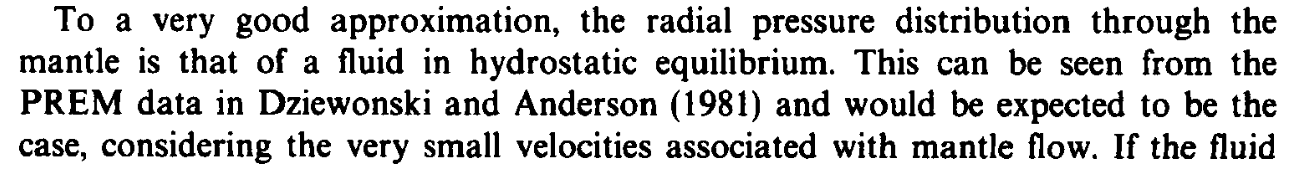
\includegraphics[width=14cm]{images/sope_06}}
\fbox{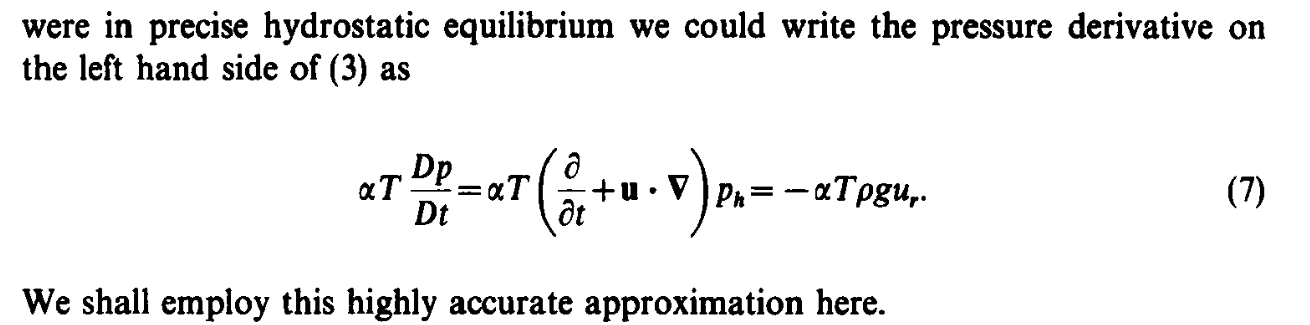
\includegraphics[width=14cm]{images/sope_07}}\cite{sope90}\\
{\tiny Note that this is indeed an approximation. ASPECT offers the choice of using the 
left or right term. The approximation has the advantage to rid the term from the full 
pressure, which could be numerically welcome, since the left term involves all three
main unknowns, i.e. velocity, pressure and temperature.}
\end{center}


In the following paragraph they justify that the inertial term $\rho Dv/Dt$ 
can be set to zero:
\begin{center}
\fbox{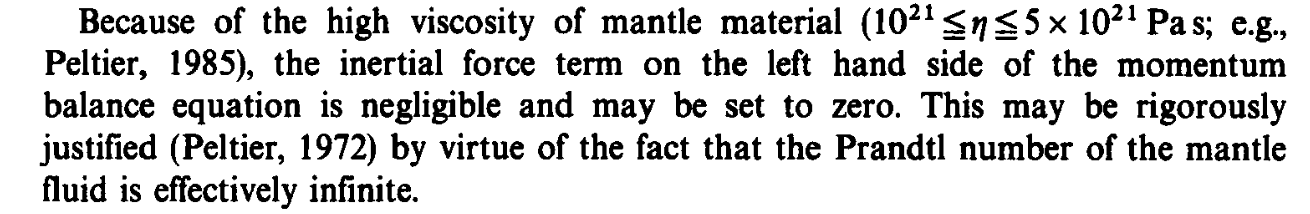
\includegraphics[width=14cm]{images/sope_08}}\cite{sope90}\\
{\tiny indeed, see section \ref{ss:nondim}.}
\end{center}

The authors justify that the gravity is assumed to be constant inside the mantle:
\begin{displayquote}
{\color{darkgray}
The gravitational acceleration, $\vec{g}$, is also taken to be constant. Since the
acceleration due to gravity, g, does not differ from 10.1 m/s by more than 6\%
throughout the entire mantle (\cite{dzan81}, 1981), we will set 
$\vec{g}= -g \vec{e}_r$, with $g$ constant.
}
\end{displayquote}

It looks like the nondimensionalisation is somewhat different than most 
of the later works we will encounter:
\begin{center}
\fbox{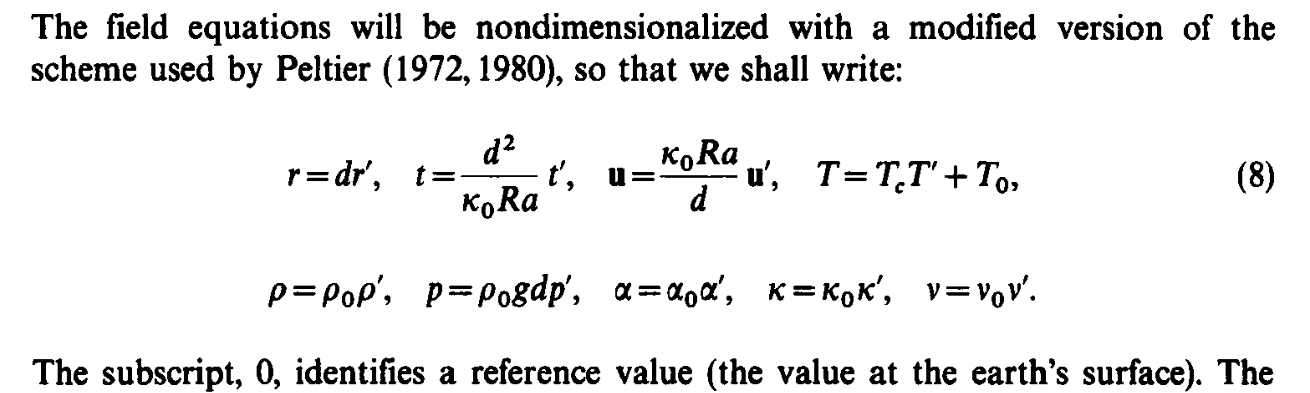
\includegraphics[width=14cm]{images/sope_09}}\cite{sope90}
\end{center}
It also leads to a different set of equations:
\begin{center}
\fbox{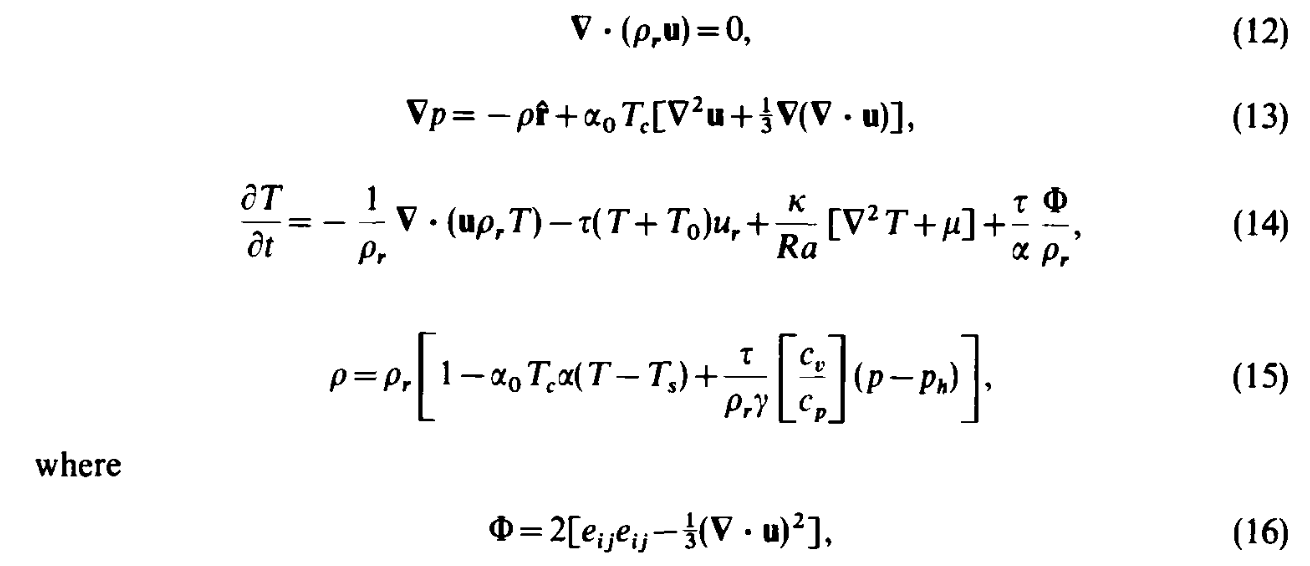
\includegraphics[width=14cm]{images/sope_10}}\cite{sope90}
\end{center}











\newpage
%%%%%%%%%%%%%%%%%%%%%%%%%%%%%%%%%%%%%%%%%%%%%%%%%%%%%%%%%%%%%%%%%%%%%%%%%%%%
\subsection{Ita \& King (1994) \label{ss:dimeqs4}}

We start from \cite{itki94} (1994).

\begin{center}
\fbox{
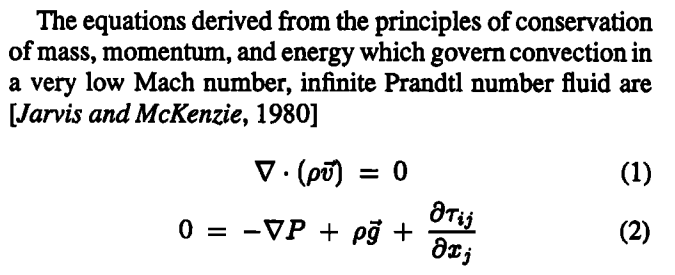
\includegraphics[width=8cm]{images/itki_01}
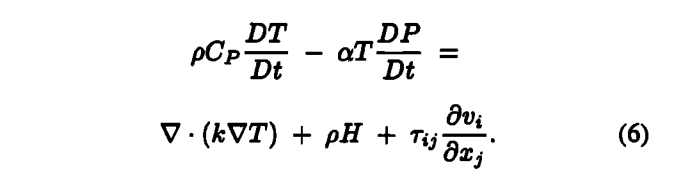
\includegraphics[width=8cm]{images/itki_02}}\cite{itki94}\\
{\tiny These are indeed the standard mass, momentum , energy conservation
equations as presented in Jarvis \& McKenzie 1980.}
\end{center}

\begin{center}
\fbox{
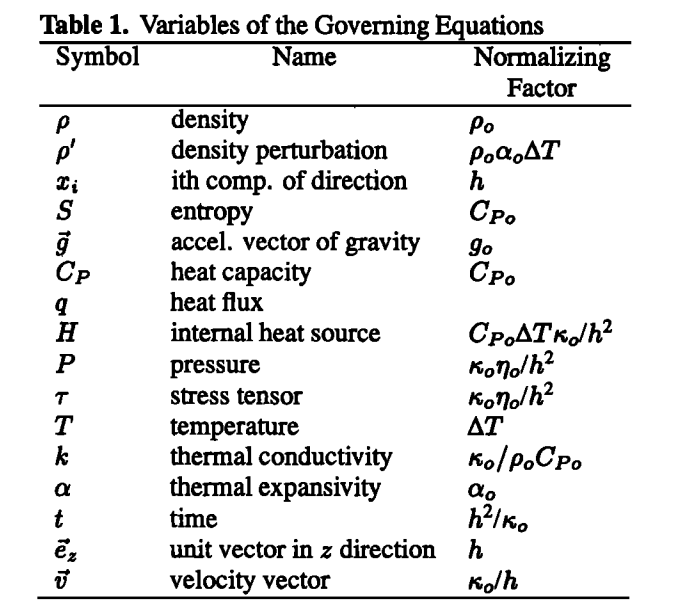
\includegraphics[width=8cm]{images/itki_03}
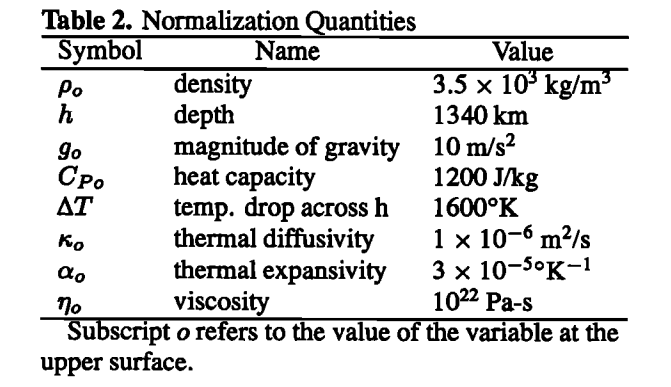
\includegraphics[width=8cm]{images/itki_13}}\cite{itki94}
\end{center}

Note that there is a different normalising factor for $\rho$ and $\rho'$!
Also, and more importantly, the definition of the heat diffusivity is $\kappa = k/ \rho C_p$, 
so that the normalizing factor of $k$ in the left table should be read $\kappa_0 \rho_0 C_{p0}$.

{\color{red} {\bf Q}: why {\it these} specific normalizing factors?}

\vspace{0.5cm}

\begin{center}
\fbox{
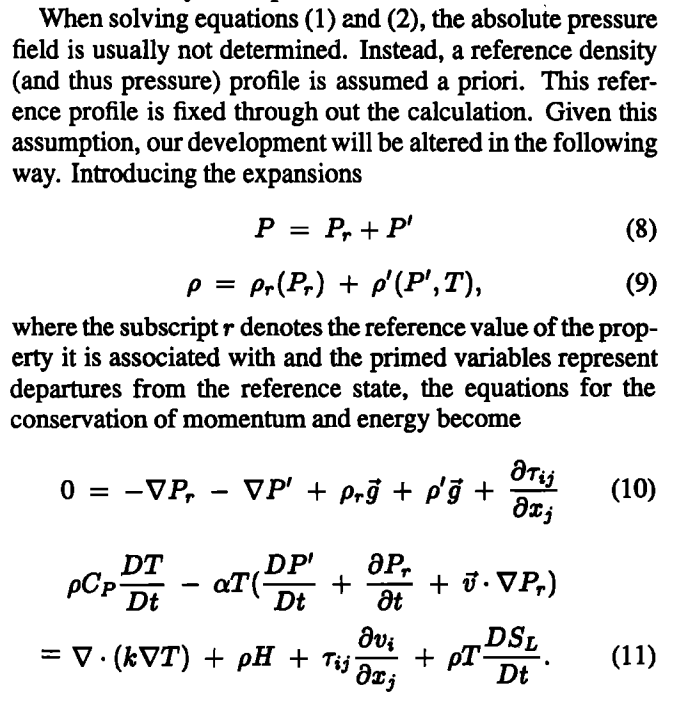
\includegraphics[width=8cm]{images/itki_04}
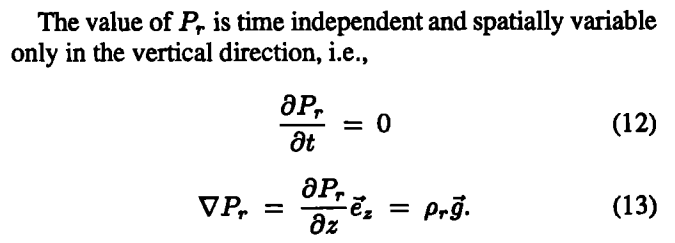
\includegraphics[width=8cm]{images/itki_05}}\cite{itki94}
\end{center}

\begin{center}
\fbox{
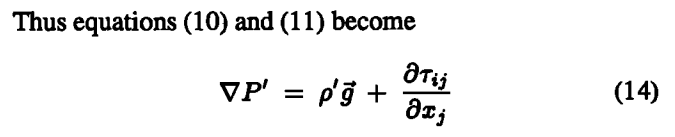
\includegraphics[width=8cm]{images/itki_06}
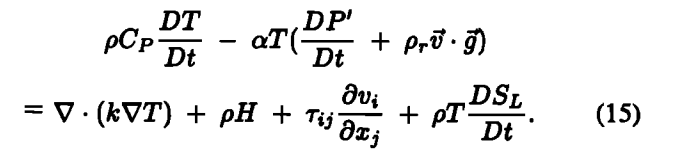
\includegraphics[width=8cm]{images/itki_07}}\cite{itki94}
\end{center}

\begin{center}
\fbox{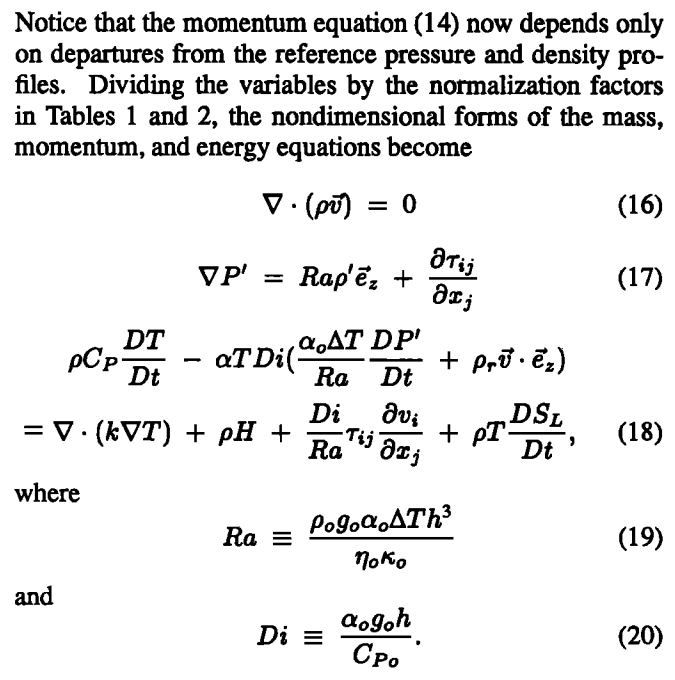
\includegraphics[width=8cm]{images/itki_08}}
\end{center}

The equations above (16,17,18) are not derived in the article so I will do so hereafter, discarding the entropy change term $S_L$.
In what follows all dimensionless quantities are of this {\color{teal} color} and $\underline{X}$
stands for the normalizing factor of the quantity $X$.

Obviously, because of the zero rhs of Eq.(16) we can immediately write
\[
{\color{teal} \vec\nabla } \cdot  ({\color{teal} \rho \vec\upnu}) = 0
\]
We then proceed to the momentum equation (14) which I rewrite without index notations:
\[
-\vec\nabla p' + \vec\nabla \cdot {\bm \tau} + \rho' \vec{g} = \vec{0}
\]
We then divide this by the normalizing factor for stress/pressure from Table 1, i.e. 
$\underline{p}=\kappa_0 \eta_0/h^2$:
\[
-\vec\nabla {\color{teal}p'} + \vec\nabla \cdot {\color{teal} {\bm \tau}} 
+ \frac{h^2}{\kappa_0 \eta_0}\rho' \vec{g} = \vec{0}
\]
We then use the normalising factor for gravity $\underline{g}=g_0$ and 
for density $\underline{\rho}' =\rho_0 \alpha_0 \Delta T$:
\[
-\vec\nabla {\color{teal}p'} + \vec\nabla \cdot {\color{teal} {\bm \tau}} 
+ \frac{h^2}{\kappa_0 \eta_0} \rho_0 \alpha \Delta T g_0 {\color{teal} \rho' \vec{g}} = \vec{0}
\]
Finally, since ${\color{teal} \vec\nabla} = h \vec\nabla $
we obtain
\[
-\frac{1}{h} {\color{teal} \vec\nabla} {\color{teal}p'} 
+ \frac{1}{h} {\color{teal} \vec\nabla} \cdot {\color{teal} {\bm \tau}} 
+ \frac{h^2 \rho_0 \alpha \Delta T g_0 }{\kappa_0 \eta_0} {\color{teal} \rho' \vec{g}} = \vec{0}
\]
Using the definition of the Rayleigh number $\Ranb$ we arrive at Eq.(17) of the paper:
\[
-{\color{teal} \vec\nabla} {\color{teal}p} + {\color{teal} \vec\nabla} \cdot 
{\color{teal} {\bm \tau}}
+ \Ranb  {\color{teal} \rho' \vec{g}} =\vec{0} 
\]


Note that ${\color{teal} \vec{g}}$ is the unit vector pointing in the direction 
of the gravity. The authors use $\vec{e}_z$ which is equal to ${\color{teal} \vec{g}}$ 
only if the $z$ axis point downwards.

An now the energy equation:

\[
\rho C_p \frac{DT}{Dt} 
- \alpha T \left( \frac{Dp'}{Dt} + \rho_r \vec\upnu \cdot \vec{g} \right)
= \vec\nabla \cdot k \vec\nabla T
+ \rho H 
+ {\bm \tau} : \vec\nabla \vec\upnu
\]
Let us consider each term one by one:

\begin{eqnarray}
\rho C_p \frac{DT}{Dt}
&=& 
\frac{\underline{\rho} \underline{C_p} \underline{T} }{\underline{t}}
{\color{teal} \rho C_p \frac{DT}{Dt}} 
= \frac{\rho_0 C_{p0} \Delta T \kappa_0}{h^2}
{\color{teal} \rho C_p \frac{DT}{Dt}} 
\nn\\
\nn\\
\alpha T 
&=& \underline{\alpha}\underline{T} {\color{teal} \alpha T } 
= \alpha_0 \Delta T {\color{teal} \alpha T } 
\nn\\
\nn\\
\frac{Dp'}{Dt} 
&=&
\frac{\underline{p}}{\underline{t}} {\color{teal} \frac{Dp'}{Dt} } 
= \frac{ \kappa_0^2 \eta_0}{h^4 } {\color{teal} \frac{Dp'}{Dt} } 
\nn\\
\nn\\
\rho_r \vec\upnu \cdot \vec{g} 
&=& 
\underline{\rho} \underline{\upnu}\underline{g}
{\color{teal} \rho_r \vec\upnu \cdot \vec{g} } 
=
\frac{\rho_0 \kappa_0 g_0}{h }
{\color{teal} \rho_r \vec\upnu \cdot \vec{g} } 
\nn\\
\nn\\
\vec\nabla \cdot k \vec\nabla T
&=& 
\frac{\underline{k} \underline{T}}{\underline{L}^2}
{\color{teal} \vec\nabla \cdot k \vec\nabla T} 
=
\frac{\kappa_0 \rho_0 C_{p0} \Delta T}{h^2}
{\color{teal} \vec\nabla \cdot k \vec\nabla T}
\nn\\
\nn\\
{\bm \tau} : \vec\nabla \vec\upnu
&=& \frac{\underline{p} \underline{\upnu}}{\underline{L}}
{\color{teal} {\bm \tau} : \vec\nabla \vec\upnu} 
=
\frac{\kappa_0^2 \eta_0}{h^4}
{\color{teal} {\bm \tau} : \vec\nabla \vec\upnu} 
\nn\\
\nn\\
\rho H 
&=& 
\underline{\rho} \underline{H} 
{\color{teal} \rho H }
=\frac{\rho_0 C_{p0} \Delta T \kappa_0 }{h^2}
{\color{teal} \rho H } \nn
\end{eqnarray}
Putting it all together:


\[
\frac{\rho_0 C_{p0} \Delta T \kappa_0}{h^2}
{\color{teal} \rho C_p \frac{DT}{Dt}} 
-
\alpha_0 \Delta T {\color{teal} \alpha T } 
\left(
\frac{ \kappa_0^2 \eta_0}{h^4 } {\color{teal} \frac{Dp'}{Dt} } 
+
\frac{\rho_0 \kappa_0 g_0}{h }
{\color{teal} \rho_r \vec\upnu \cdot \vec{g} } 
\right)
=
\frac{\kappa_0 \rho_0 C_{p0} \Delta T}{h^2}
{\color{teal} \vec\nabla \cdot k \vec\nabla T}
+
\frac{\rho_0 C_{p0} \Delta T \kappa_0 }{h^2}
{\color{teal} \rho H }
+
\frac{\kappa_0^2 \eta_0}{h^4}
{\color{teal} {\bm \tau} : \vec\nabla \vec\upnu} 
\]
Next step is to divide all terms by $\kappa_0$:
\[
\frac{\rho_0 C_{p0} \Delta T }{h^2}
{\color{teal} \rho C_p \frac{DT}{Dt}} 
-
\alpha_0 \Delta T {\color{teal} \alpha T } 
\left(
\frac{ \kappa_0 \eta_0}{h^4 } {\color{teal} \frac{Dp'}{Dt} } 
+
\frac{\rho_0  g_0}{h }
{\color{teal} \rho_r \vec\upnu \cdot \vec{g} } 
\right)
=
\frac{ \rho_0 C_{p0} \Delta T}{h^2}
{\color{teal} \vec\nabla \cdot k \vec\nabla T}
+
\frac{\rho_0 C_{p0} \Delta T  }{h^2}
{\color{teal} \rho H }
+
\frac{\kappa_0 \eta_0}{h^4}
{\color{teal} {\bm \tau} : \vec\nabla \vec\upnu} 
\]
Then we multiply by $\frac{h^2}{\rho_0 C_{p0} \Delta T }$:
\[
{\color{teal} \rho C_p \frac{DT}{Dt}} 
-
\frac{h^2}{\rho_0 C_{p0}  }\alpha_0  {\color{teal} \alpha T } 
\left(
\frac{ \kappa_0 \eta_0}{h^4 } {\color{teal} \frac{Dp'}{Dt} } 
+
\frac{\rho_0  g_0}{h }
{\color{teal} \rho_r \vec\upnu \cdot \vec{g} } 
\right)
=
{\color{teal} \vec\nabla \cdot k \vec\nabla T}
+
{\color{teal} \rho H }
+
\frac{\kappa_0 \eta_0}{\rho_0 C_{p0} \Delta T  h^2}
{\color{teal} {\bm \tau} : \vec\nabla \vec\upnu} 
\]
Since
\[
\frac{\Dinb}{\Ranb} = \frac{\alpha_0 g_0 h}{C_{p0}} 
\frac{\eta_0 \kappa_0}{\rho_0 g_0 \alpha_0 \Delta T h^3}
= \frac{\eta_0 \kappa_0}{C_{p0} \rho_0 \Delta T  h^2}
\]
we can then write 
\[
{\color{teal} \rho C_p \frac{DT}{Dt}} 
-
\frac{h^2}{\rho_0 C_{p0}  }\alpha_0  {\color{teal} \alpha T } 
\left(
\frac{ \kappa_0 \eta_0}{h^4 } {\color{teal} \frac{Dp'}{Dt} } 
+
\frac{\rho_0  g_0}{h }
{\color{teal} \rho_r \vec\upnu \cdot \vec{g} } 
\right)
=
{\color{teal} \vec\nabla \cdot k \vec\nabla T}
+
{\color{teal} \rho H }
+
\frac{\Dinb}{\Ranb} 
{\color{teal} {\bm \tau} : \vec\nabla \vec\upnu} 
\]
We then extract $\rho_0 g_0/h$ from the parenthesis:
\[
{\color{teal} \rho C_p \frac{DT}{Dt}} 
-
\frac{h^2}{\rho_0 C_{p0}  }\alpha_0  {\color{teal} \alpha T } 
\frac{\rho_0  g_0}{h }
\left(
\frac{h}{\rho_0  g_0}
\frac{ \kappa_0 \eta_0}{h^4 } {\color{teal} \frac{Dp'}{Dt} } 
+
{\color{teal} \rho_r \vec\upnu \cdot \vec{g} } 
\right)
=
{\color{teal} \vec\nabla \cdot k \vec\nabla T}
+
{\color{teal} \rho H }
+
\frac{\Dinb}{\Ranb} 
{\color{teal} {\bm \tau} : \vec\nabla \vec\upnu} 
\]
\[
{\color{teal} \rho C_p \frac{DT}{Dt}} 
- \frac{\alpha_0 g_0 h }{ C_{p0}  }  {\color{teal} \alpha T } 
\left( \frac{ \kappa_0 \eta_0}{h^3 \rho_0  g_0} {\color{teal} \frac{Dp'}{Dt} } 
+{\color{teal} \rho_r \vec\upnu \cdot \vec{g} }  \right)
=
{\color{teal} \vec\nabla \cdot k \vec\nabla T}
+
{\color{teal} \rho H }
+
\frac{\Dinb}{\Ranb} 
{\color{teal} {\bm \tau} : \vec\nabla \vec\upnu} 
\]
We have 
\[
\frac{\alpha_0 \Delta T}{\Ranb} = 
\frac{\alpha_0 \Delta T \eta_0 \kappa_0}{\rho_0 g_0 \alpha_0 \Delta T h^3} = 
\frac{\eta_0 \kappa_0}{\rho_0 g_0   h^3} 
\qquad
\text{and}
\qquad
\Dinb = \frac{\alpha_0 g_0 h}{C_{p0}} 
\]
so that finally
\[
{\color{teal} \rho C_p \frac{DT}{Dt}} 
- \Dinb  {\color{teal} \alpha T } 
\left( 
\frac{\alpha_0 \Delta T}{\Ranb}
{\color{teal} \frac{Dp'}{Dt} } 
+{\color{teal} \rho_r \vec\upnu \cdot \vec{g} }  \right)
=
{\color{teal} \vec\nabla \cdot k \vec\nabla T}
+
{\color{teal} \rho H }
+
\frac{\Dinb}{\Ranb} 
{\color{teal} {\bm \tau} : \vec\nabla \vec\upnu} 
\]
which is indeed Eq.(18) of the article.

\newpage
\subsubsection{ALA}
To recap, the equations above are the so-called ALA equations as mentioned in 
the article 
\begin{displayquote}  {\color{darkgray}
The present form of the equations is generally recognized
as the anelastic liquid approximation (ALA).}
\end{displayquote}

\begin{center}
\fbox{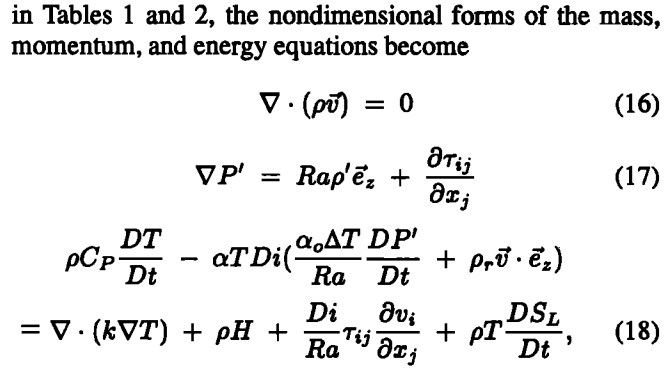
\includegraphics[width=8cm]{images/itki_12}}\cite{itki94}
\end{center}

which I rewrite again hereafter:
\begin{eqnarray}
{\color{teal} \vec\nabla } \cdot  ({\color{teal} \rho \vec\upnu}) &=& 0 \nn\\
-{\color{teal} \vec\nabla} {\color{teal}p} + {\color{teal} \vec\nabla} \cdot 
{\color{teal} {\bm \tau}}
+ \Ranb  {\color{teal} \rho' \vec{g}} &=&\vec{0} \nn\\
{\color{teal} \rho C_p \frac{DT}{Dt}} 
- \Dinb  {\color{teal} \alpha T } 
\left( 
\frac{\alpha_0 \Delta T}{\Ranb}
{\color{teal} \frac{Dp'}{Dt} } 
+{\color{teal} \rho_r \vec\upnu \cdot \vec{g} }  \right)
&=&
{\color{teal} \vec\nabla \cdot k \vec\nabla T}
+
{\color{teal} \rho H }
+
\frac{\Dinb}{\Ranb} 
{\color{teal} {\bm \tau} : \vec\nabla \vec\upnu} 
\end{eqnarray}

However, we read in \cite{vacp22}: 
\begin{displayquote}  {\color{darkgray}
The anelastic liquid approximation (ALA; 
\cite{jamc80}, 1980) assumes that lateral density variations are
small relative to a reference density profile and can be neglected in the mass equation  and energy conservation equation, which instead use the density of the
depth-dependent reference profile. Only the buoyancy term
in the momentum equation uses a temperature- and pressure-dependent density, which is approximated using 
a Taylor expansion. }
\end{displayquote}


Also, when we look in \cite{lezh08} (I come back to this article in Section~\ref{complezh08}):
\begin{center}
\fbox{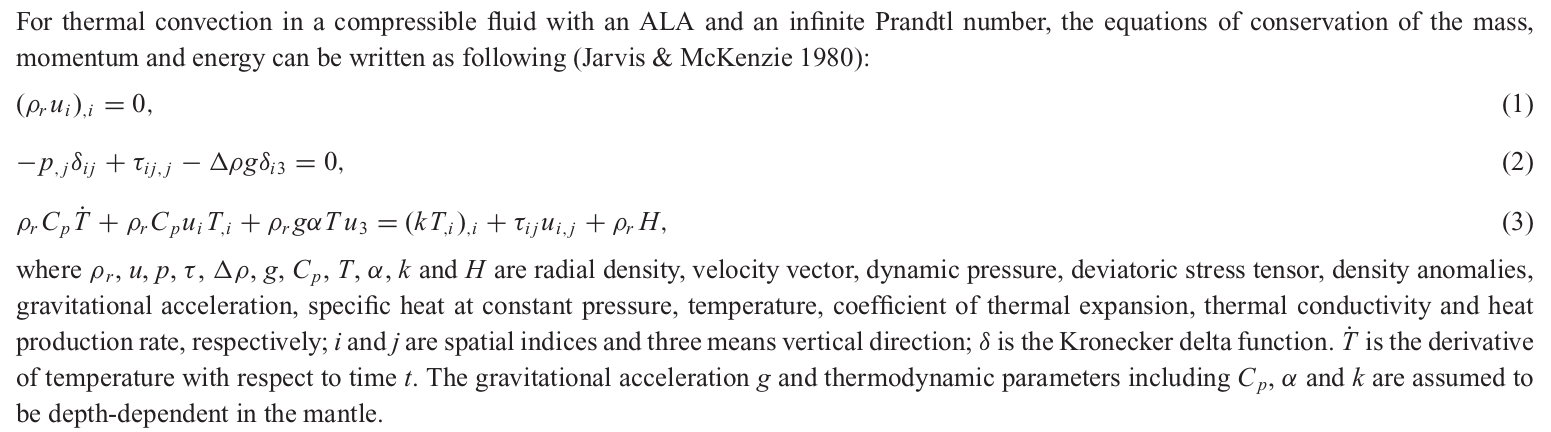
\includegraphics[width=17cm]{images/lezh_01}}
\end{center}

We find that these are in direct contradiction with the equations of Ita \& King above who use $\rho$ and not $\rho_r$ in mass and energy equations.



%------------------------------------------------------------------------
\subsubsection{TALA}
We further read in \cite{itki94}:
\begin{displayquote}  {\color{darkgray}
The next simplification of the equations disregards the term 
containing the material derivative of the nonhydrostatic pressure($P'$)
in Eq.(18) and ignores its affect on $\rho'$ in Eq.(9).}
\end{displayquote}

\fbox{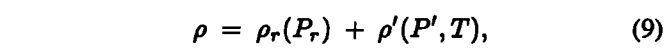
\includegraphics[width=8cm]{images/itki_10}
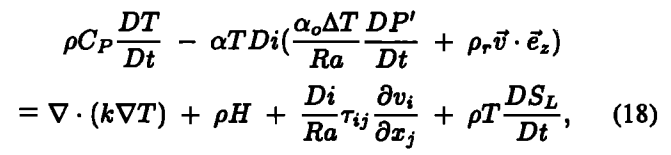
\includegraphics[width=8cm]{images/itki_11}}\cite{itki94}

Following the text above, the TALA equations are then

\begin{eqnarray}
\rho &=& \rho_r(P_r) + \rho'(T) \nn\\
{\color{teal} \vec\nabla } \cdot  ({\color{teal} \rho \vec\upnu}) &=& 0 \nn\\
-{\color{teal} \vec\nabla} {\color{teal}p} + {\color{teal} \vec\nabla} \cdot 
{\color{teal} {\bm \tau}}
+ \Ranb  {\color{teal} \rho' \vec{g}} &=&\vec{0} \nn\\
{\color{teal} \rho C_p \frac{DT}{Dt}} 
- \Dinb  {\color{teal} \alpha T } 
\left( 
{\color{teal} \rho_r \vec\upnu \cdot \vec{g} }  \right)
&=&
{\color{teal} \vec\nabla \cdot k \vec\nabla T}
+
{\color{teal} \rho H }
+
\frac{\Dinb}{\Ranb} 
{\color{teal} {\bm \tau} : \vec\nabla \vec\upnu} 
\end{eqnarray}

{\color{red} {\bf Q}: the authors state that removing $Dp'/Dt$ is a TALA thing 
but this term is absent from the ALA equations of \cite{lezh08}.:}

\fbox{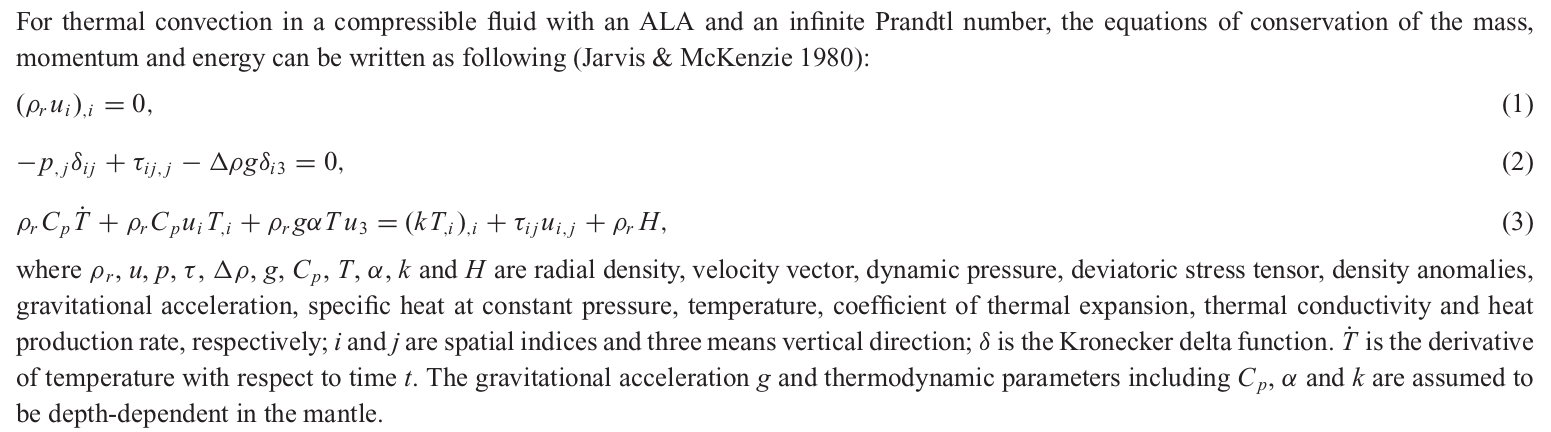
\includegraphics[width=16cm]{images/lezh_01}}\cite{lezh08}

\vspace{.5cm}

Let us further investigate the literature:
\begin{itemize}


\item We find a TALA formulation in \cite{ilkm26} (2026):
\begin{center}
\fbox{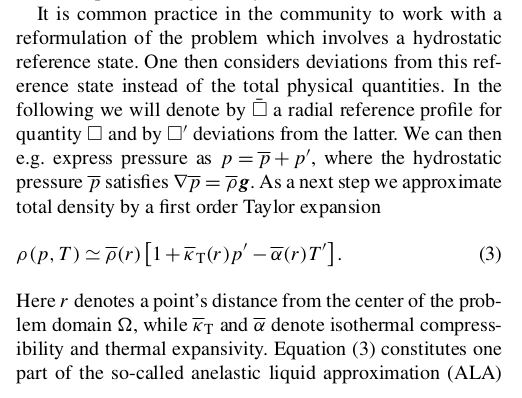
\includegraphics[width=8cm]{images/ilkm01}
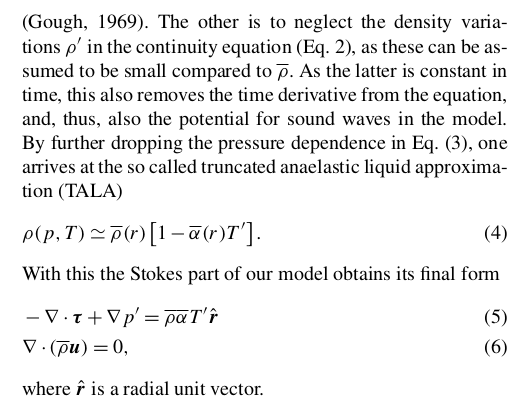
\includegraphics[width=8cm]{images/ilkm02}}\\
\fbox{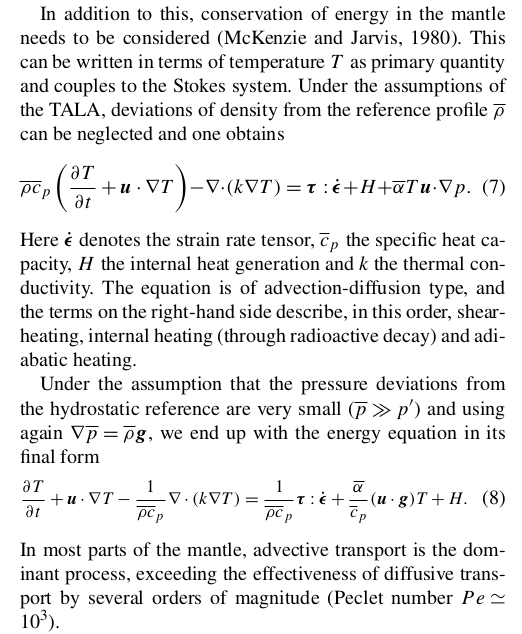
\includegraphics[width=8cm]{images/ilkm03}}\cite{ilkm26}
\end{center}

\item Likewise in \cite{kame22} we find:
\begin{center}
\fbox{
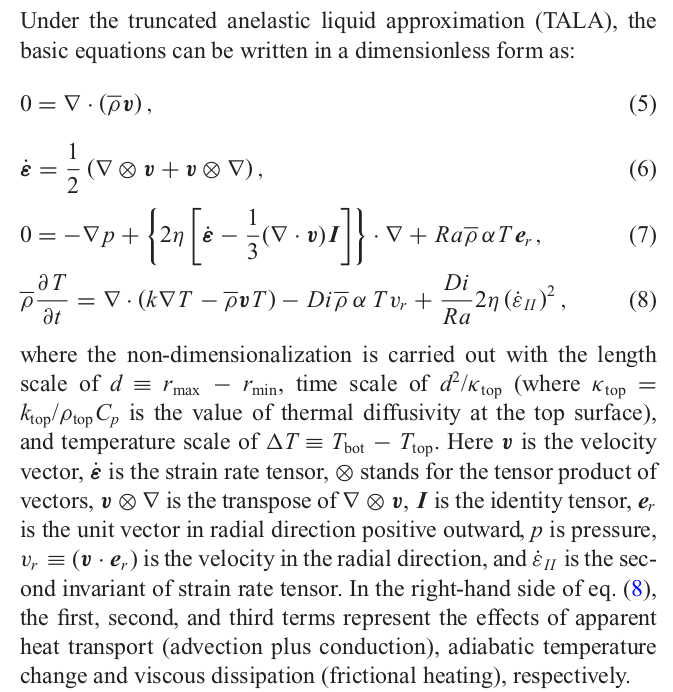
\includegraphics[width=8cm]{images/kame22a}
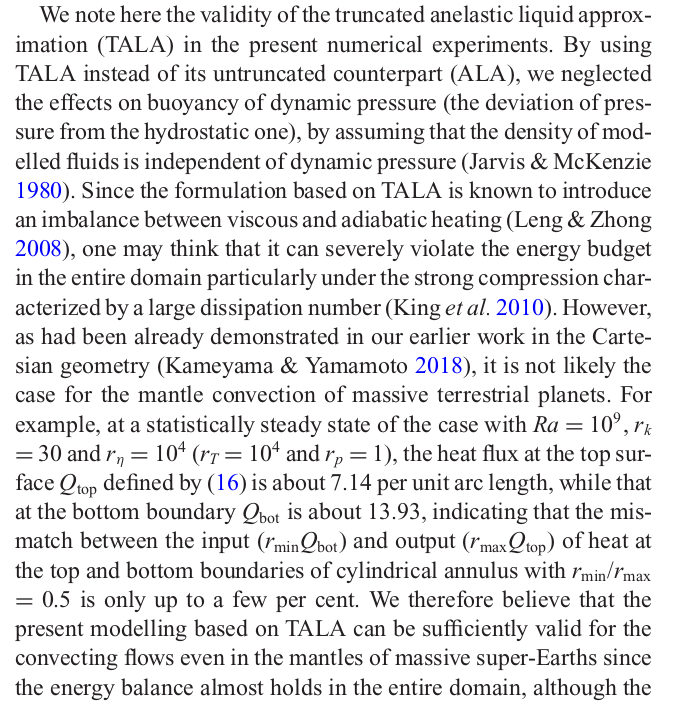
\includegraphics[width=8cm]{images/kame22b}}\\
\fbox{
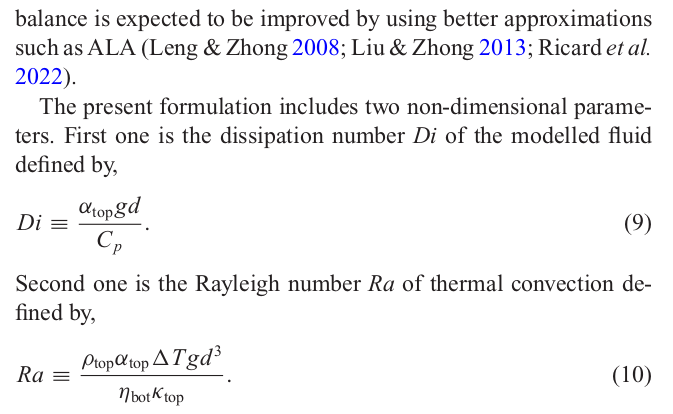
\includegraphics[width=8cm]{images/kame22c}
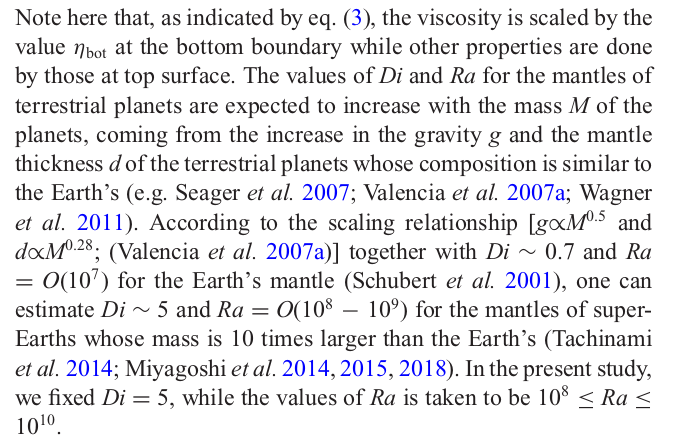
\includegraphics[width=8cm]{images/kame22d}}\\
\fbox{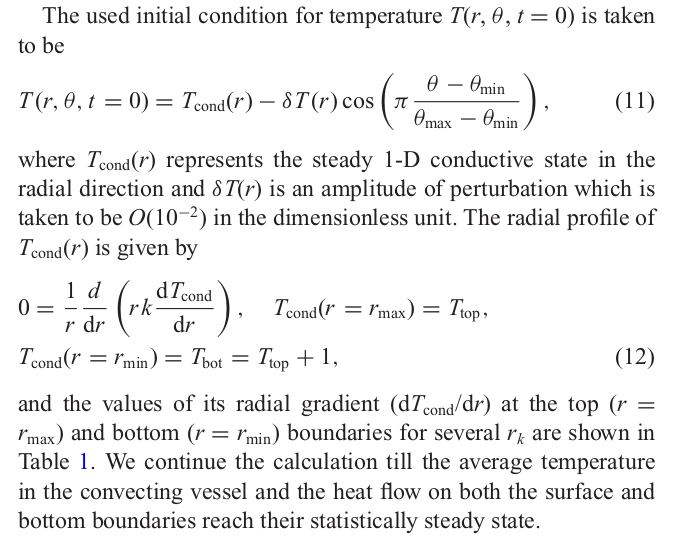
\includegraphics[width=8cm]{images/kame22e}}
\end{center}

\item Likewise in \cite{kame22} we find:
\begin{center}
\fbox{
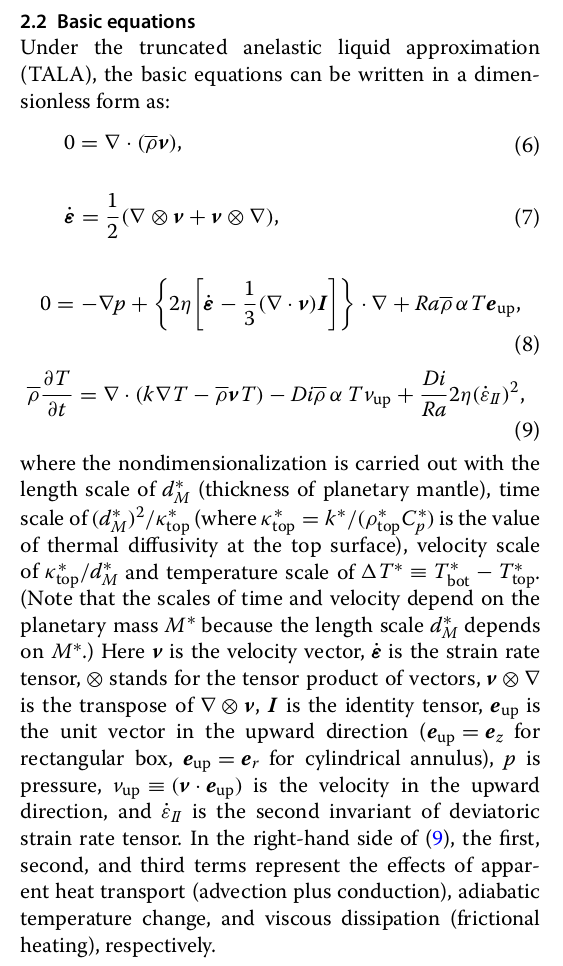
\includegraphics[width=8cm]{images/kame25a}
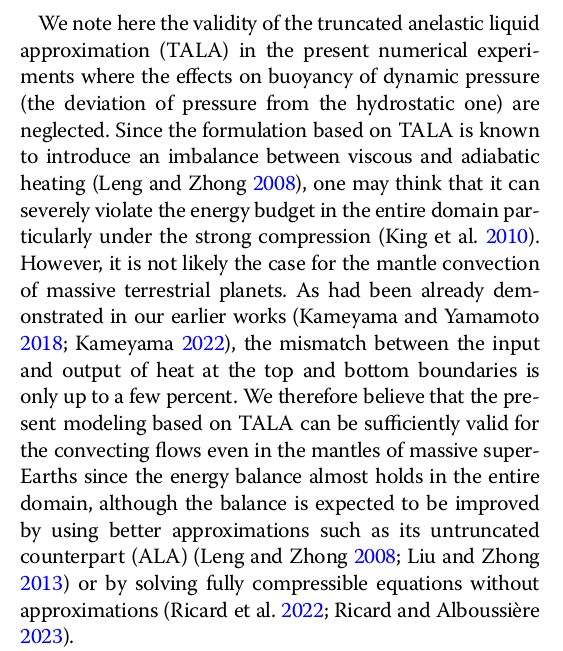
\includegraphics[width=8cm]{images/kame25b}}\\
\fbox{
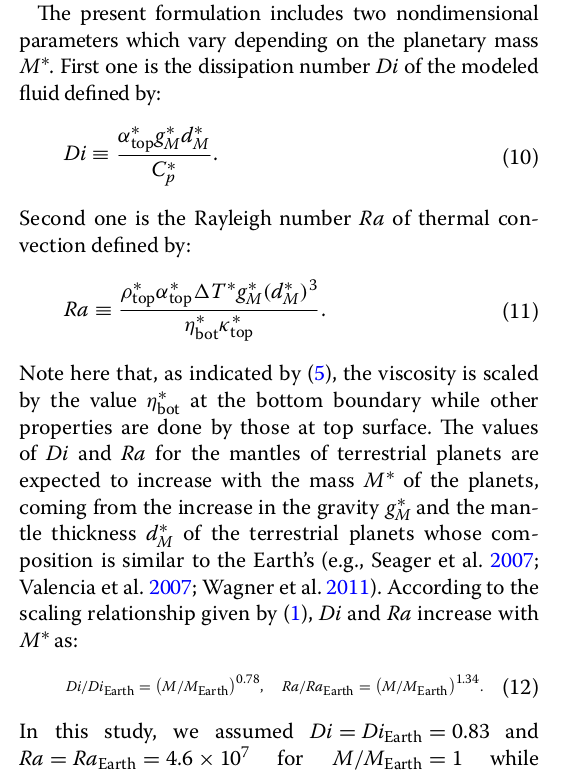
\includegraphics[width=8cm]{images/kame25c}
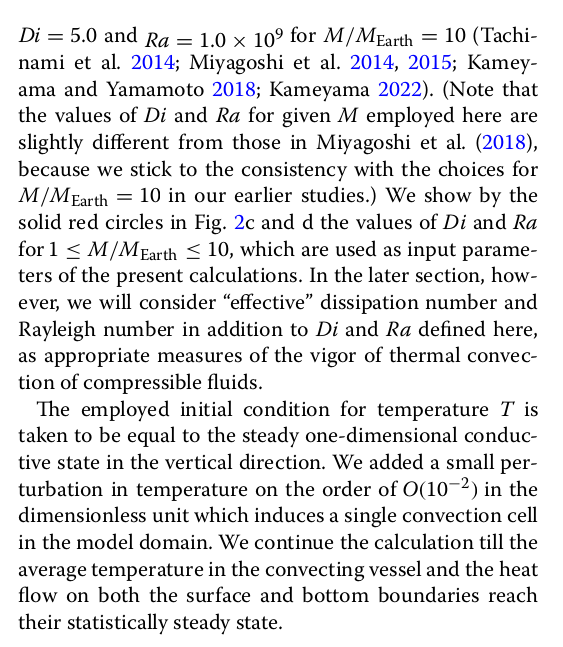
\includegraphics[width=8cm]{images/kame25d}}
\end{center}

\item finally in the 101 paper we read

\begin{displayquote} {\color{darkgray}
The truncated anelastic liquid approximation (TALA;
Jarvis and McKenzie, 1980; Ita and King, 1994) is based on
the same assumptions as the ALA but further assumes that
the variation of the density due to pressure variations can be
neglected in the buoyancy term as well. In the Earth’s mantle, these density variations are typically an order of magnitude smaller than the density changes caused by temperature.
The TALA has similar applications as ALA but introduces
an imbalance between energy dissipation calculated from the
Stokes equation and heat dissipation in the energy equation.
Consequently, it should be avoided when energy dissipation
is important in the model (Leng and Zhong, 2008; Alboussière and Ricard, 2013).}
\end{displayquote}


\end{itemize}

{\color{red} I need to conclude something!}


%------------------------------------------------------------------------
\subsubsection{EBA}

Coming back to \cite{itki94} we read in the article:
\begin{displayquote}  {\color{darkgray}
A further common reduction is known as the extended Boussinesq approximation (EBA).
Under the EBA, the reference density profile is assumed to be single valued 
[$\rho_r \rightarrow \rho_0$]. Because the expected thermal perturbations are small,
normalized density is assumed to be unity in equation 16 and 18 
[ $\rho \rightarrow \rho_0$, i.e. ${\color{teal} \rho} \rightarrow 1$, in mass and energy equations]}
\end{displayquote}

\begin{eqnarray}
\rho &=& \rho_0 + \rho'(T) \nn\\
{\color{teal} \vec\nabla } \cdot  {\color{teal}  \vec\upnu} &=& 0 \nn\\
-{\color{teal} \vec\nabla} {\color{teal}p} + {\color{teal} \vec\nabla} \cdot 
{\color{teal} {\bm \tau}}
+ \Ranb  {\color{teal} \rho' \vec{g}} &=&\vec{0} \nn\\
{\color{teal}  C_p \frac{DT}{Dt}} 
- \Dinb  {\color{teal} \alpha T } 
\left( 
{\color{teal} \rho_0 \vec\upnu \cdot \vec{g} }  \right)
&=&
{\color{teal} \vec\nabla \cdot k \vec\nabla T}
+
{\color{teal} \rho H }
+
\frac{\Dinb}{\Ranb} 
{\color{teal} {\bm \tau} : \vec\nabla \vec\upnu} 
\end{eqnarray}

This form of the continuity equation implies that the flow is incompressible. 

{\color{red} {\bf Q}: does this agree with other sources?}


%------------------------------------------------------------------------
\subsubsection{BA}

Finally:
\begin{displayquote}  {\color{darkgray}
The simplest form of the equations is known as the Boussinesq
approximation (BA). In this form, all the terms in the 
EBA equations containing the  Dissipation number ($\Dinb$) are dropped.}
\end{displayquote}

\begin{eqnarray}
\rho &=& \rho_0 + \rho'(T) \nn\\
{\color{teal} \vec\nabla } \cdot  {\color{teal}  \vec\upnu} &=& 0 
\nn\\
-{\color{teal} \vec\nabla} {\color{teal}p} + {\color{teal} \vec\nabla} \cdot 
{\color{teal} {\bm \tau}}
+ \Ranb  {\color{teal} \rho' \vec{g}} &=&\vec{0} 
\nn\\
{\color{teal}  C_p \frac{DT}{Dt}} 
&=&
{\color{teal} \vec\nabla \cdot k \vec\nabla T}
+
{\color{teal} \rho H }
\end{eqnarray}


The Boussinesq approximation is examined in detail in \cite{spve60} (1960).

We read in \cite{tack96} (1996):
\begin{displayquote} {\color{darkgray}
The Boussinesq approximation [Boussinesq, 1903; Rayleigh, 1916], 
in which density is assumed constant
except for weak variations with temperature which appear in
the buoyancy term of the momentum equation, and (usually)
material properties are assumed constant, has commonly been
used in studies of mantle convection. Numerical simulations
and laboratory experiments on Boussinesq fluids with constant
material properties at moderate Rayleigh numbers ($\Ranb$) in
rectangular Cartesian boxes have indicated that many
different convective patterns are possible at a particular $\Ranb$,
depending on the initial conditions, size of box, boundary
conditions,and heating mode.
}
\end{displayquote}




\newpage
%%%%%%%%%%%%%%%%%%%%%%%%%%%%%%%%%%%%%%%%%%%%%%%%%%%%%%%%%%%%%%%%%%%
\subsection{Leng \& Zhong (2008)}\label{complezh08}

For reference we recall again the 101 paper \cite{vacp22}: 
\begin{displayquote} {\color{darkgray}
The anelastic liquid approximation (ALA; 
\cite{jamc80}, 1980) assumes that lateral density variations are
small relative to a reference density profile and can be neglected in the mass equation  and energy conservation equation, which instead use the density of the
depth-dependent reference profile. Only the buoyancy term
in the momentum equation in Eq. (5) uses a temperature-
and pressure-dependent density, which is approximated using 
a Taylor expansion. This approximation is commonly used in 
whole-mantle convection models,
wherein the density changes substantially from the surface to
the core–mantle boundary, and compressibility is an important 
effect. Its use is appropriate as long as deviations from
the reference profile remain small or are not important for
the interpretation of the model. For example, substantial expansion or contraction caused by temperature changes that 
are not on the reference profile, such as cooling or heating in
the thermal boundary layers caused by conduction, and the
stresses caused by this process cannot be modelled with this
approximation. Phase transitions of different types of materials 
can also cause large density or temperature changes, since
only one type of material can be represented by the reference
profile.}
\end{displayquote}

\vspace{0.5cm}

Warning: in what follows the domain is a Cartesian box with $z$ being the vertical axis 
pointing upwards.

\begin{center}
\fbox{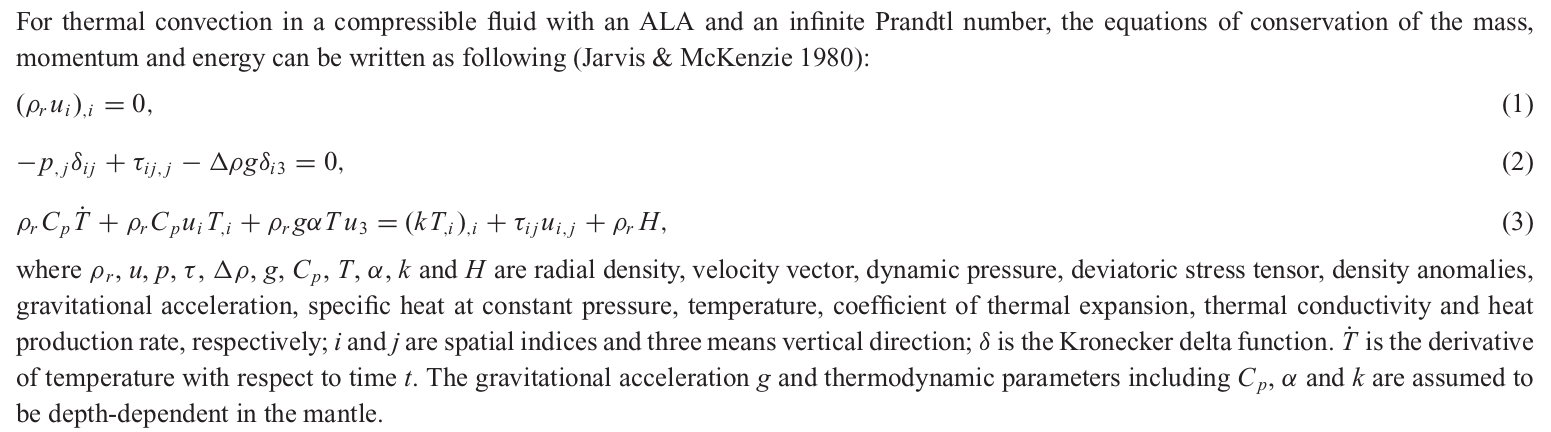
\includegraphics[width=17cm]{images/lezh_01}}\cite{lezh08}
\end{center}

I here assume $\vec{g}=-g \vec{e}_z$, so that the equations above can be written without index notations as follows:

\begin{eqnarray}
\vec\nabla \cdot ( \rho_r \vec\upnu ) &=& 0 \nn\\
-\vec\nabla p + \vec\nabla \cdot {\bm \tau} + \Delta\rho \; \vec{g} &=& \vec{0} \nn\\
\rho_r C_p \left(  \frac{\partial T}{\partial t} + \vec\upnu \cdot \vec\nabla T \right)
&=& \vec\nabla \cdot (k \vec\nabla T) + {\bm \tau} : {\vec\nabla \vec\upnu} +
\rho_r \alpha T \vec\upnu \cdot \vec{g}   + \rho_r H
\end{eqnarray}

Note that the fact that the buoyancy term contains $\Delta \rho$ and not the full 
pressure means that the computed pressure is the dynamic pressure. 

\begin{center}
\fbox{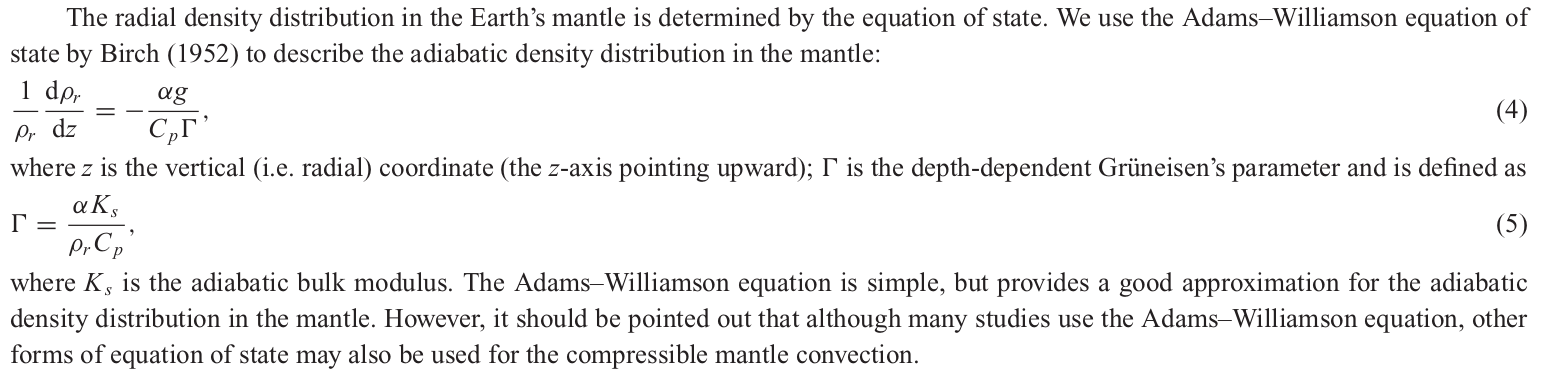
\includegraphics[width=17cm]{images/lezh_02}}\cite{lezh08}
\end{center}

\[
\frac{1}{\rho_r} \frac{d \rho_r}{dz} = - \frac{\alpha g}{C_p \Gamma}
\qquad
\text{with}
\qquad  
\Gamma = \frac{\alpha K_s}{\rho_r C_p}
\]

In \cite{jamc80} (1980) we find:
\[
\Gamma = \frac{\alpha K_s}{\rho C_p} = \frac{\alpha K_T } {\rho C_v}
\]
where $K_s$ and $K_T$ are the isentropic and isothermal moduli of bulk compressibility
and $C_v$, is the specific heat at constant volume. 
These assumptions are made to simplify
the mathematics and to reduce the number of variables of the problem. [...]
For most liquids, $\Gamma$ is approximately constant and of order 1.
Assuming $\Gamma$ to be constant eliminates the bulk moduli as independent parameters.
{\color{red} is this a quote?}

\begin{center}
\fbox{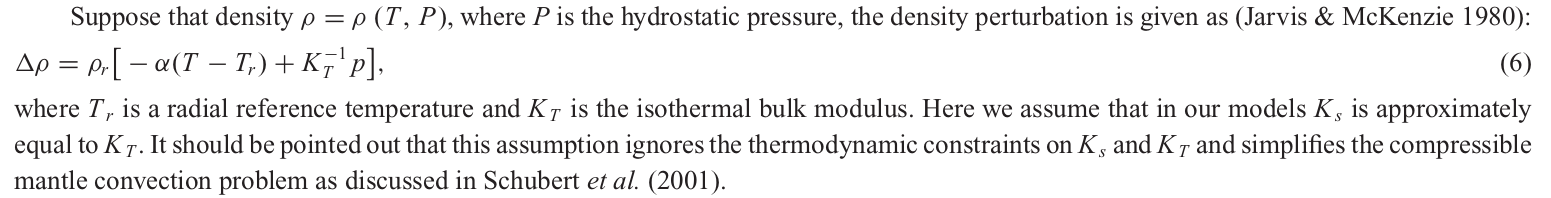
\includegraphics[width=17cm]{images/lezh_03}}\cite{lezh08}
\end{center}

\[
\Delta \rho = \rho_r \left[ -\alpha (T-T_r) + K_T^{-1} p \right]
\]

\begin{center}
\fbox{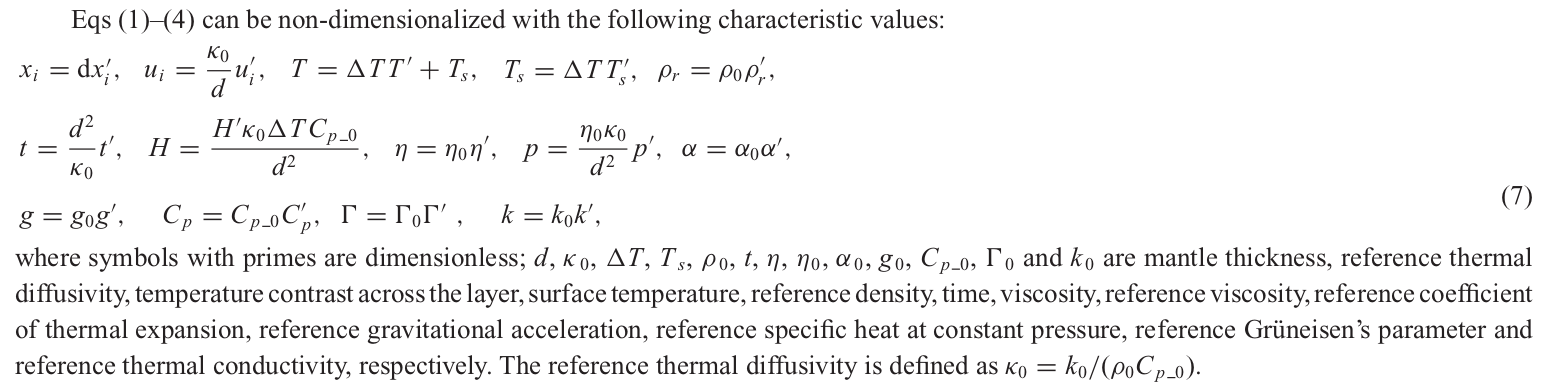
\includegraphics[width=17cm]{images/lezh_04}}\cite{lezh08}
\end{center}

\begin{center}
\fbox{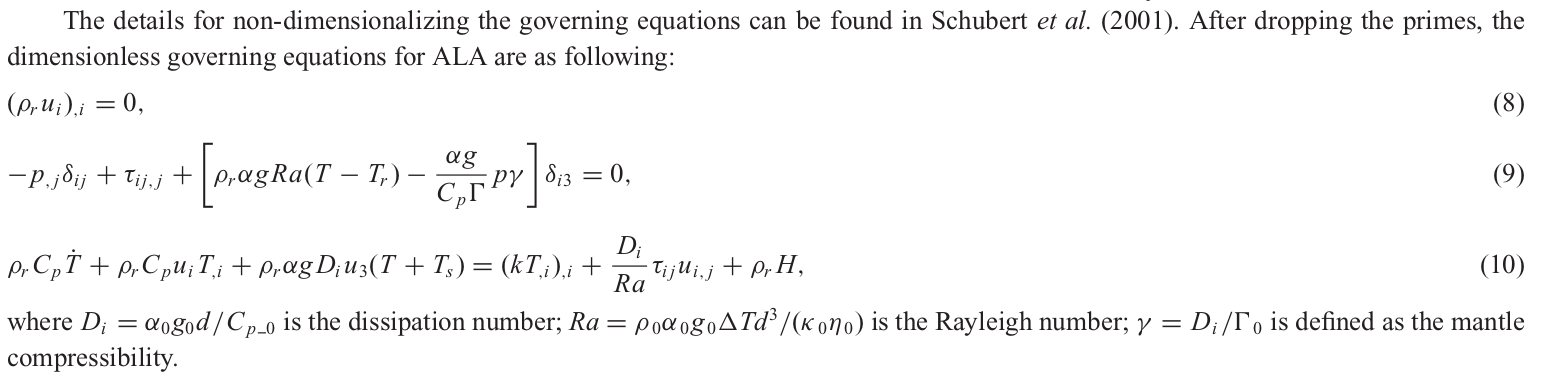
\includegraphics[width=17cm]{images/lezh_05}}\cite{lezh08}
\end{center}

\begin{eqnarray}
\vec\nabla  \cdot ( \rho_r \vec\upnu) &=& 0 \nn\\
-\vec\nabla p + \vec\nabla \cdot {\bm \tau} + 
\left[
\rho_r \alpha g \Ranb (T-T_r) - \frac{\alpha g}{C_p \Gamma} p \gamma
\right] \vec{e}_z
\Delta\rho \; \vec{g} &=& \vec{0} 
\nn\\
\rho_r C_p \left(  \frac{\partial T}{\partial t} + \vec\upnu \cdot \vec\nabla T \right)
&=& \vec\nabla \cdot (k \vec\nabla T) + 
\frac{\Dinb}{\Ranb} {\bm \tau} : {\vec\nabla \vec\upnu} 
+ \rho_r \alpha \Dinb (T+T_s) \vec\upnu \cdot \vec{g}   + \rho_r H \nonumber
\end{eqnarray}

I need to check the momentum equation, minus sign ?

\[
\Dinb = \frac{\alpha_0 g_0 d}{C_{p,0}} 
\qquad
\Ranb = \frac{\rho_0 \alpha_0 g_0 \Delta T d^3}{\kappa_0 \eta_0}
\qquad
\gamma = \frac{\Dinb}{\Gamma_0}
\]

\begin{center}
\fbox{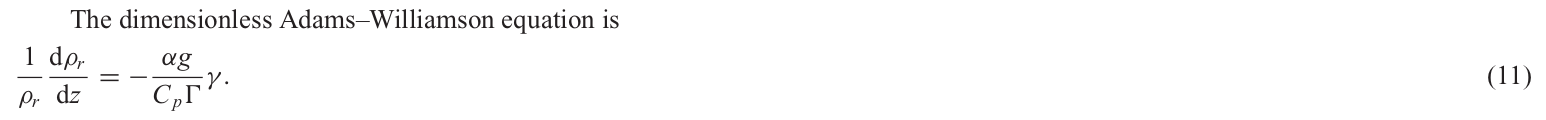
\includegraphics[width=17cm]{images/lezh_06}}\cite{lezh08}
\end{center}
\[
\frac{1}{\rho_r} \frac{d \rho_r}{dz} = - \frac{\alpha g}{C_p \Gamma} \gamma
\]
\begin{center}
\fbox{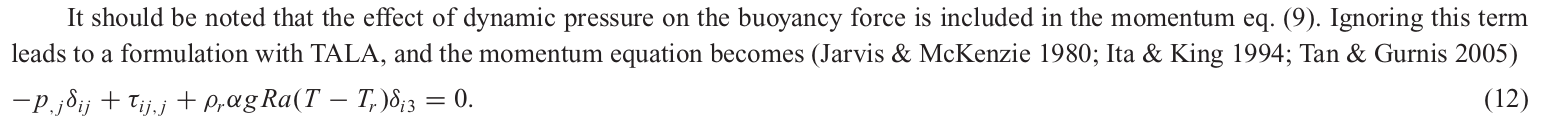
\includegraphics[width=17cm]{images/lezh_07}}\cite{lezh08}
\end{center}
\[
-\vec\nabla p + \vec\nabla \cdot {\bm \tau} +  ...
\]


101 paper: ``
The truncated anelastic liquid approximation (TALA;
Jarvis and McKenzie, 1980; Ita and King, 1994) is based on
the same assumptions as the ALA but further assumes that
the variation of the density due to pressure variations can be
neglected in the buoyancy term as well. In the Earth’s mantle, these density variations are typically an order of magnitude smaller than the density changes caused by temperature.
The TALA has similar applications as ALA but introduces
an imbalance between energy dissipation calculated from the
Stokes equation and heat dissipation in the energy equation.
Consequently, it should be avoided when energy dissipation
is important in the model (Leng and Zhong, 2008; Alboussière and Ricard, 2013).
''

\vspace{1cm}
\begin{center}
\fbox{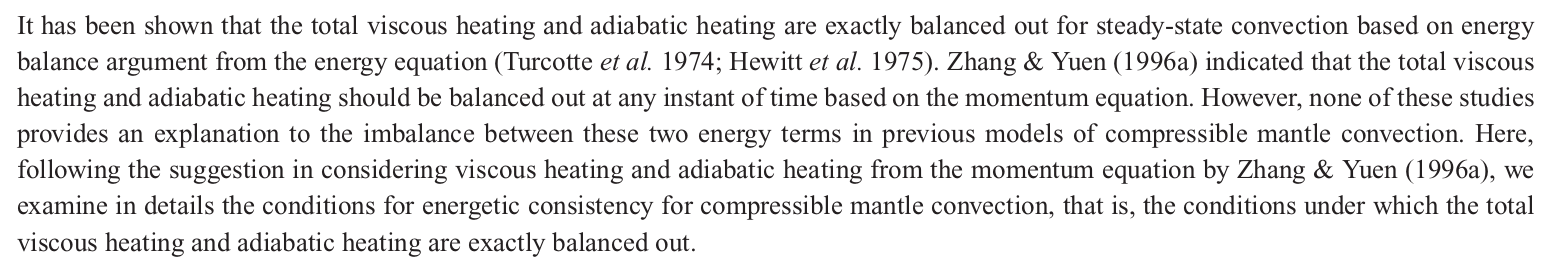
\includegraphics[width=17cm]{images/lezh_08}}\cite{lezh08}
\end{center}
\begin{center}
\fbox{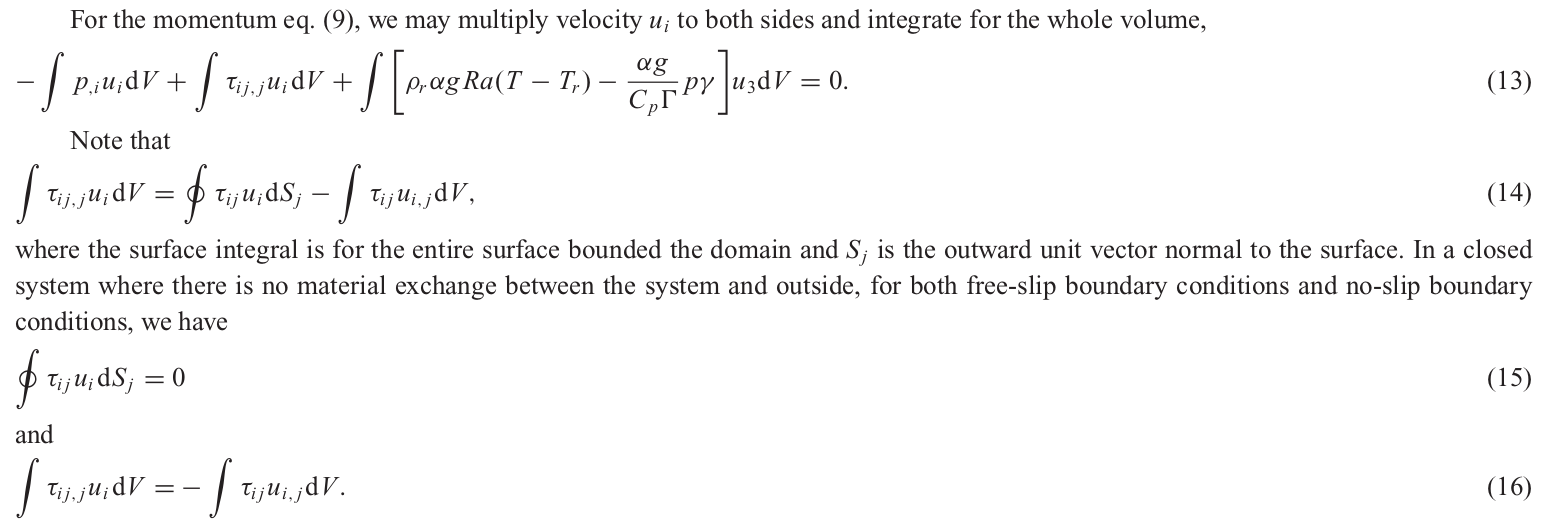
\includegraphics[width=17cm]{images/lezh_09}}\cite{lezh08}
\end{center}

\begin{eqnarray}
-\int \vec\nabla p \cdot \vec\upnu \; dV
+ 
\int (\vec\nabla  \cdot {\bm \tau} ) \cdot \vec\upnu \; dV 
+ 
\int \left[
..
\right] \vec{e}_z \cdot \vec\upnu \; dV=0 \nn\\
\int (\vec\nabla \cdot {\bm \tau} ) \cdot \vec\upnu \; dV 
= \underbrace{ \int ({\bm \tau}\cdot \vec\upnu) \cdot \vec{n} \; dS }_{=0 (b.c.)}
-\int {\bm \tau} : \vec\nabla\vec\upnu\; dV 
\end{eqnarray}

\fbox{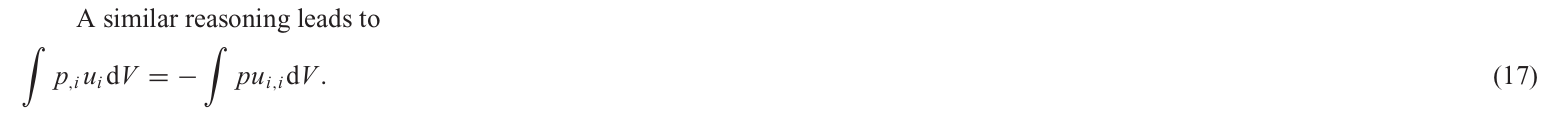
\includegraphics[width=16cm]{images/lezh_10}}

\[
\int \vec\nabla p \cdot \vec\upnu \; dV
= - \int p \vec\nabla \cdot \vec\upnu \; dV
\]

\fbox{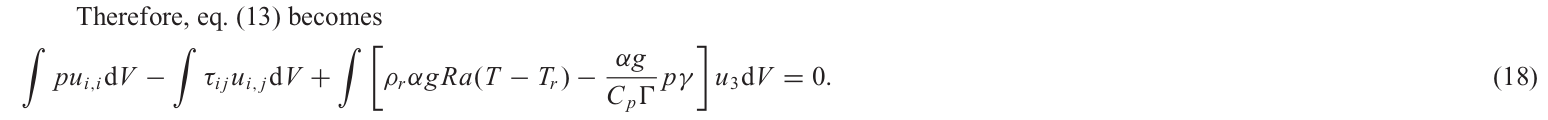
\includegraphics[width=16cm]{images/lezh_11}}

\[
\int p \vec\nabla \cdot \vec\upnu \; dV
-
\int {\bm \tau} : \vec\nabla\vec\upnu\; dV
+
\int ...dV =0
\]

\fbox{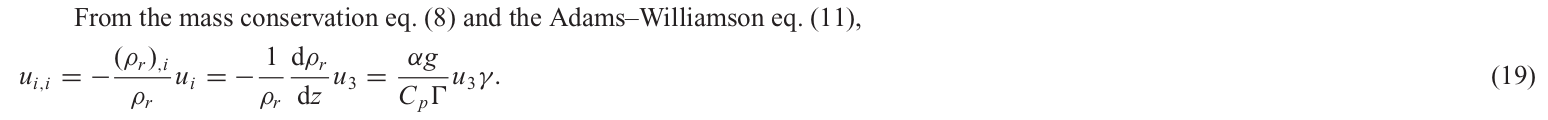
\includegraphics[width=16cm]{images/lezh_12}}

\begin{eqnarray}
\vec\nabla  \cdot ( \rho_r \vec\upnu) &=& 0 \nn\\
\Rightarrow \rho_r \vec\nabla\cdot \vec\upnu + \vec\upnu \cdot \vec\nabla \rho_r &=& 0 \nn\\
\Rightarrow \vec\nabla \cdot \vec\upnu &=& - \frac{\vec\nabla \rho_r }{\rho_r} \cdot \vec\upnu \nn\\
\Rightarrow \vec\nabla \cdot \vec\upnu &=& - \frac{1}{\rho_r}\frac{d\rho_r}{dz} \upnu_z \nn\\
\Rightarrow \vec\nabla \cdot \vec\upnu &=& \frac{\alpha g}{C_p \Gamma} \gamma \upnu_z \nn
\end{eqnarray}
where we have assumed that $\rho_r$ is a function of $z$ only.

\fbox{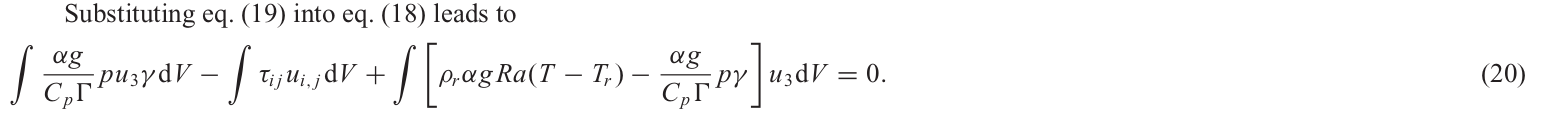
\includegraphics[width=16cm]{images/lezh_13}}

\[
\int p \frac{\alpha g}{C_p \Gamma} \gamma \upnu_z  \; dV
-
\int {\bm \tau} : \vec\nabla\vec\upnu\; dV
+
\int [... ]dV =0
\]

\fbox{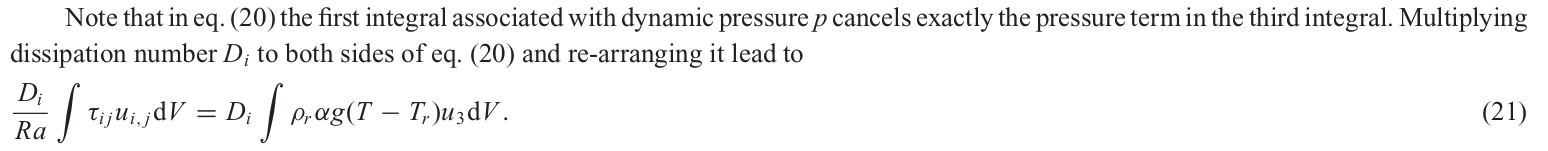
\includegraphics[width=16cm]{images/lezh_14}}

\[
\frac{\Dinb}{\Ranb}\int {\bm \tau} : \vec\nabla\vec\upnu\; dV
= 
\Dinb \int \rho_r \alpha g (T-T_r) \upnu_z \; dV
\]

\fbox{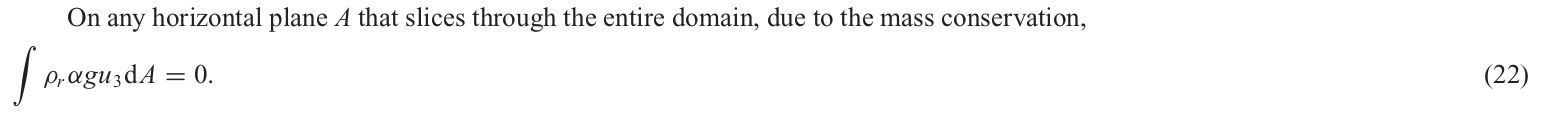
\includegraphics[width=16cm]{images/lezh_15}}

\[
\int \rho_r \alpha g \upnu_z \; dA =0
\]



\newpage
%%%%%%%%%%%%%%%%%%%%%%%%%%%%%%%%%%%%%%%%%%%%%%%%%%%%%%%%%%%%%%%%%%%%%%%
\subsection{Tan \& Gurnis (2007)}

One very interesting aspect of this publication is the fact that 
the authors also explain the FEM discretisation \& implementation of the equations,
as well as the structure of the solver.

The authors start from the TALA approximation:

\begin{center}
\fbox{
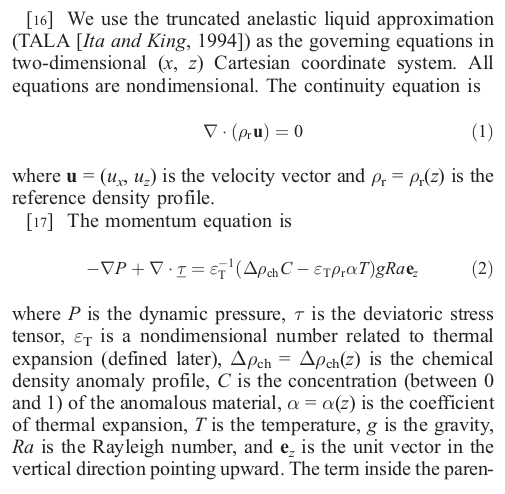
\includegraphics[width=8cm]{images/tagu07a}
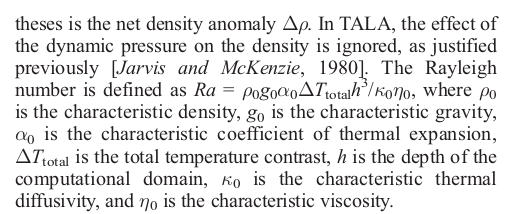
\includegraphics[width=8cm]{images/tagu07b}}
\end{center}

\begin{center}
\fbox{
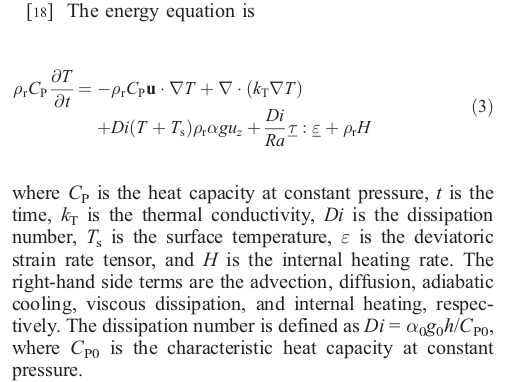
\includegraphics[width=8cm]{images/tagu07c}
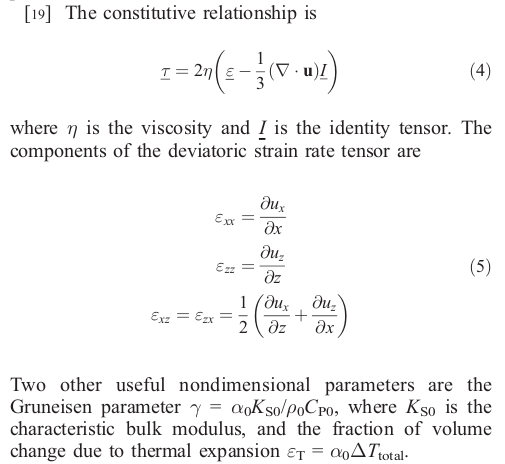
\includegraphics[width=8cm]{images/tagu07d}}
\end{center}

The authors then proceed to explain how they adapted ConMan (a 2d $Q_1\times P_0$ penalty-formulation based FE code) to accommodate compressible flow.

\begin{center}
\fbox{
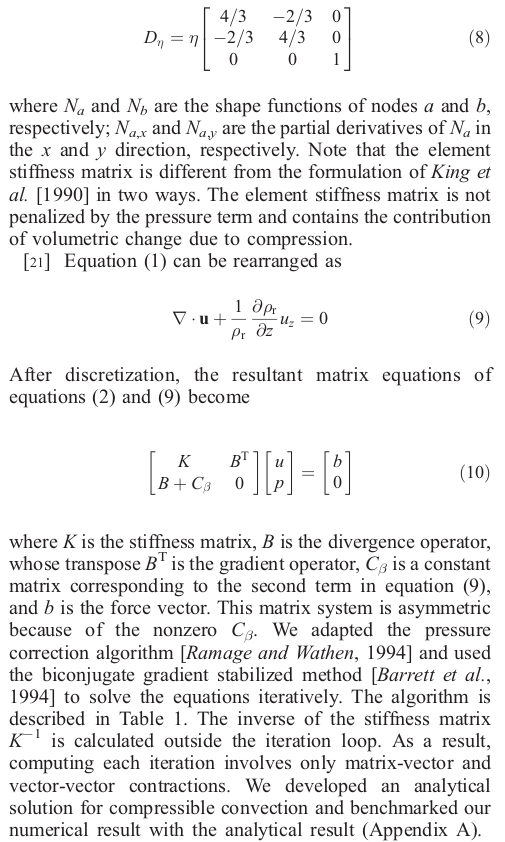
\includegraphics[width=8cm]{images/tagu07f}
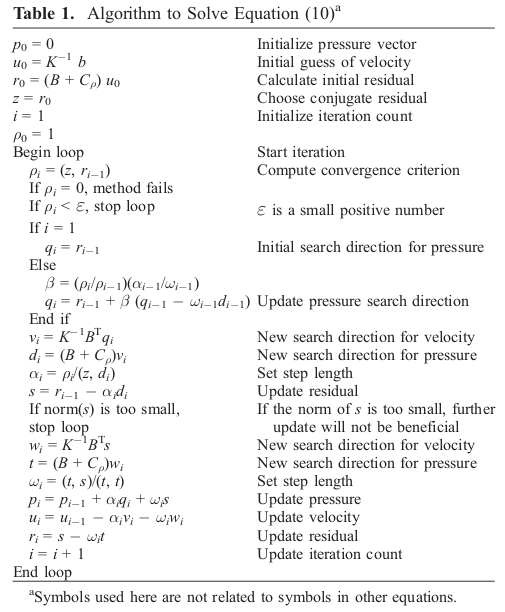
\includegraphics[width=8cm]{images/tagu07g}}
\end{center}



\newpage
%%%%%%%%%%%%%%%%%%%%%%%%%%%%%%%%%%%%%%%%%%%%%%%%%%%%%%%%%%%%%%%%%%%%%%%
\subsection{King et al (2010)}

This article is very interesting because it presents a 
community benchmark for 2-D Cartesian compressible convection.
The article starts by presenting the set of standard equations:

\begin{center}
\fbox{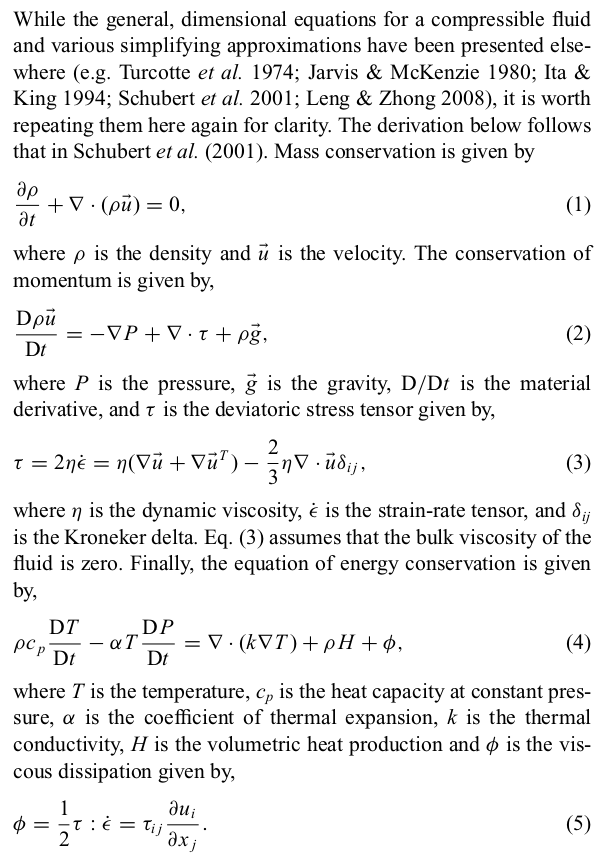
\includegraphics[width=8cm]{images/kilv10a}}
\end{center}

I have no real comment about these except that Eq.2 should read $\rho D\vec\upnu/Dt$?
Where it gets more interesting is what follows:

\begin{center}
\fbox{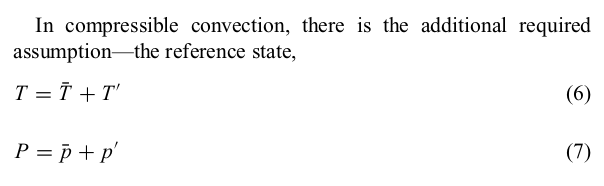
\includegraphics[width=8cm]{images/kilv10b}}
\fbox{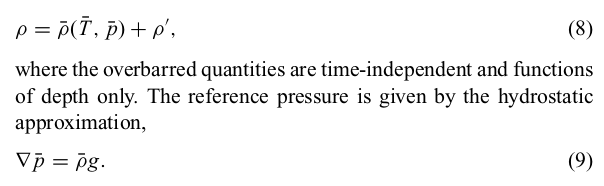
\includegraphics[width=8cm]{images/kilv10c}}
\end{center}

Temperature, pressure and density are split in radial reference values (overbarred) and 
deviations from them.
Then, assuming like in the paper that $p' << \overline{p}$ we can write 
\begin{eqnarray}
\frac{Dp}{Dt}
&\simeq& \frac{D\overline{p}}{Dt} \nn\\
&=& \frac{\partial \overline{p}}{\partial t} + \vec\upnu\cdot \vec\nabla \overline{p} \nn\\
&=&  \vec\upnu\cdot \vec\nabla \overline{p} 
\end{eqnarray}
since $\overline{p}$ is time independent. Also, $\vec\nabla \overline{p} = \overline{\rho} \vec{g}$, 
so that in the end:
\[
\frac{Dp}{Dt} \simeq  \vec\upnu \cdot \overline{\rho} \vec{g}
\]
Also, 
\begin{eqnarray}
\frac{DT}{Dt}
&=& \frac{D(\overline{T} + T'}{Dt}  \nn\\
&=& \frac{\partial (\overline{T} + T')}{\partial t} + \vec\upnu\cdot \vec\nabla (\overline{T} + T')\nn\\
&=& \frac{\partial T'}{\partial t}
+ \vec\upnu\cdot \vec\nabla  T'
+ \vec\upnu\cdot \vec\nabla \overline{T} \nn\\
&=& \frac{DT'}{Dt} + \vec\upnu\cdot \vec\nabla \overline{T} \nn
\end{eqnarray}
since $\overline{T}$ is time independent.

In the end we indeed recover the same energy equation as in the paper:
\begin{center}
\fbox{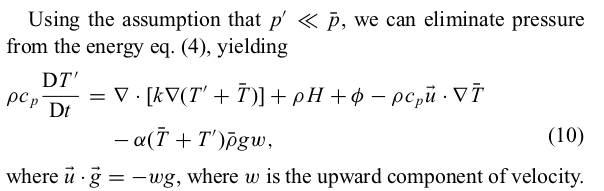
\includegraphics[width=8cm]{images/kilv10d}}
\end{center}

\begin{center}
\fbox{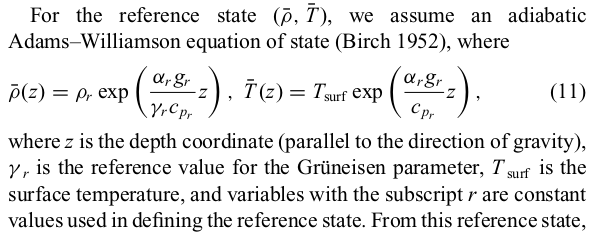
\includegraphics[width=8cm]{images/kilv10e}}
\end{center}
Please refer to Section~\ref{sec:eos} for more on equations of state.

\begin{center}
\fbox{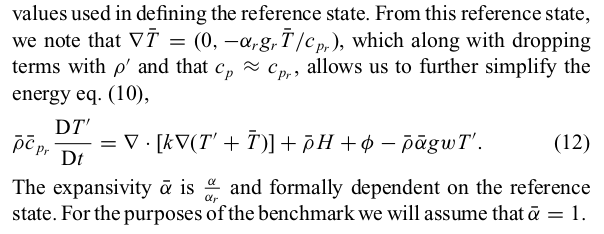
\includegraphics[width=8cm]{images/kilv10f}}
\end{center}

%-------------------------------------
\subsubsection{ALA}


\begin{center}
\fbox{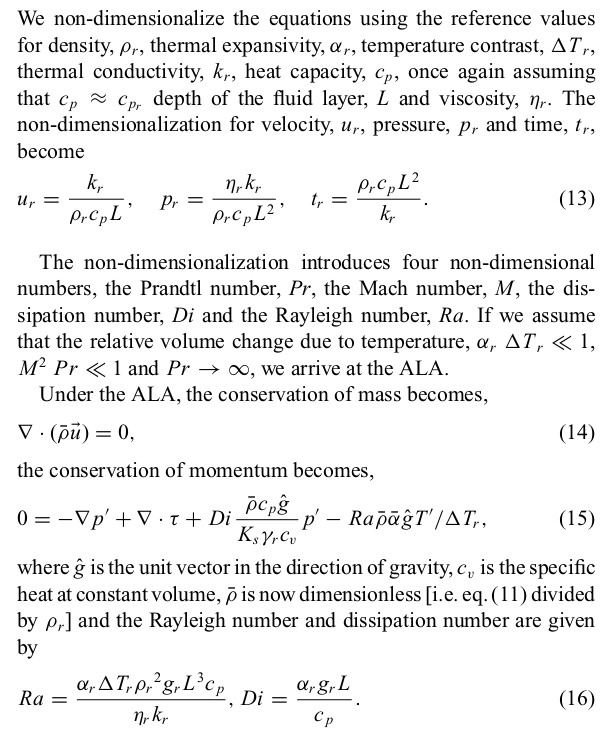
\includegraphics[width=8cm]{images/kilv10g}}
\fbox{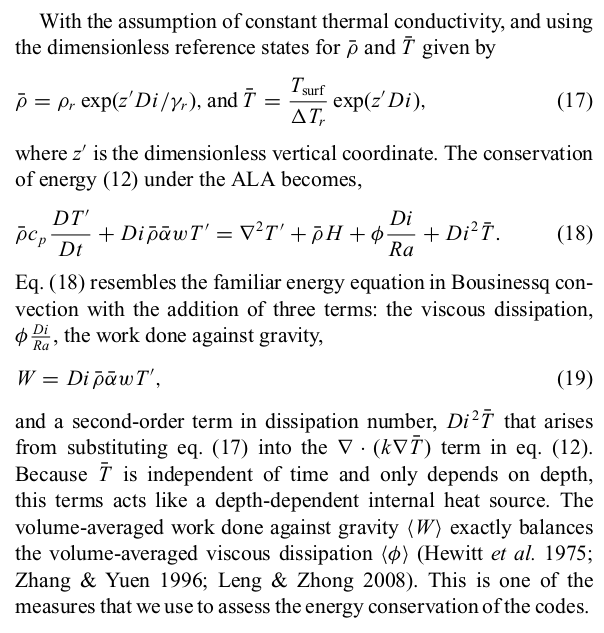
\includegraphics[width=8cm]{images/kilv10h}}
\end{center}

%-------------------------------------
\subsubsection{TALA}

\begin{center}
\fbox{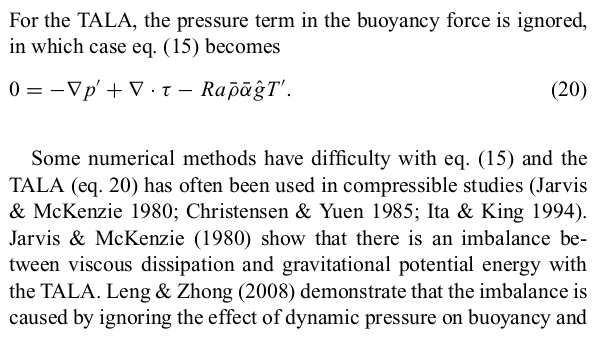
\includegraphics[width=8cm]{images/kilv10i}}
\fbox{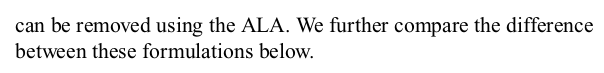
\includegraphics[width=8cm]{images/kilv10j}}
\end{center}

%-------------------------------------
\subsubsection{EBA}

\begin{center}
\fbox{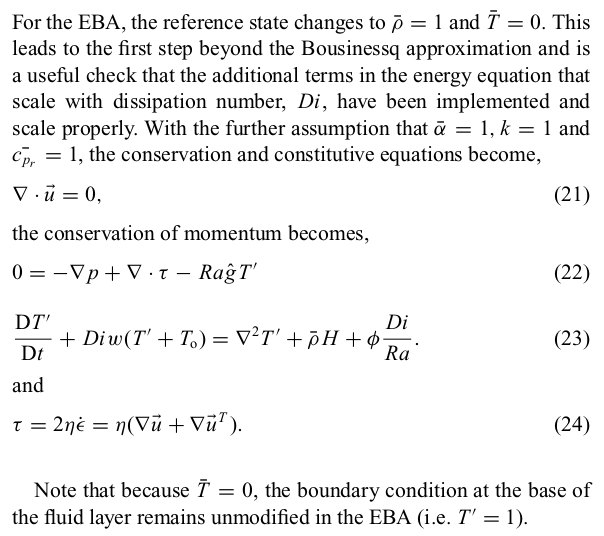
\includegraphics[width=8cm]{images/kilv10k}}
\end{center}

%-------------------------------------
\subsubsection{BA}

\begin{center}
\fbox{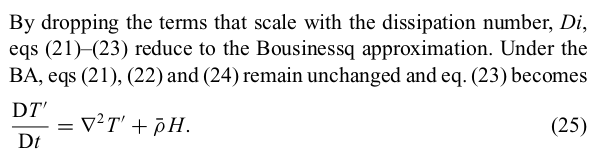
\includegraphics[width=8cm]{images/kilv10l}}
\end{center}


\newpage
%%%%%%%%%%%%%%%%%%%%%%%%%%%%%%%%%%%%%%%%%%%%%%%%%%%%%%%%%%%%%%%%%%%%%%%
\subsection{Gassm{\"o}ller et al (2020)}

Let us first recall the equations of the paper \cite{gadb20}:
\begin{center}
\fbox{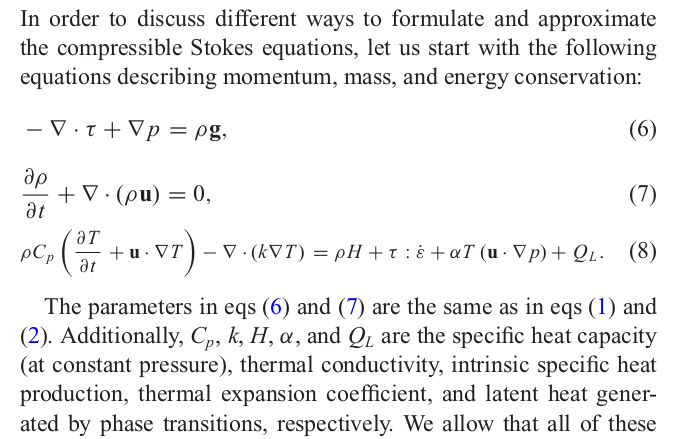
\includegraphics[width=8cm]{images/gadb20a}}
\end{center}



\subsubsection{The anelastic liquid approximation ALA}

\begin{displayquote}{\color{darkgray}
The anelastic approximation (Batchelor 1953; Ogura \& Phillips
1962; Gough 1969) or more precisely its specialization for liquids,
the anelastic liquid approximation (Jarvis \& McKenzie 1980) is
based on two assumptions.

\begin{enumerate}
\item lateral density variations are
small relative to a reference density profile: $\overline{\rho}(r) = \rho(\overline{p},\overline{T})$, where $r$ is the radial or vertical coordinate, depending on whether the model
is posed in spherical or Cartesian coordinates. The bar indicates
that density values are taken along the reference profile, and are
therefore only a function of $r$. The ALA approximates the density
via a Taylor expansion in pressure and temperature:
\[
\rho(p,T) \simeq \overline{\rho}(r) + 
\overline{\left( \frac{\partial \rho}{\partial p} \right)}_T p' +
\overline{\left( \frac{\partial \rho}{\partial T} \right)}_p T' 
=\overline{\rho}(r) \left( 1 +\overline{\kappa}_T(r) \; p' -\overline{\alpha}(r) \; T'  \right)
\]
Here, $\kappa_T$ is the isothermal compressibility, and primes mark deviations from the reference state: $p=\overline{p} + p'$  and $T=\overline{T} + T'$ .

\item the deviation of density from the
(depth-dependent) reference profile can be neglected in the mass and
energy conservation equations (7) and (8), and is only considered
in the right-hand side of the momentum conservation equation (the
buoyancy term in eq. 6), which describes the driving force of the
flow. Since this reference state is assumed to not change over time
(or to only change very slowly over time), the time-derivative of
the density in the mass conservation equation is zero, and eq. (7)
simplifies to
\[
\vec\nabla \cdot (\overline{\rho} \vec\upnu ) = 0
\]

\end{enumerate}

}
\end{displayquote}


\subsubsection{The truncated anelastic liquid approximation TALA}
\begin{displayquote}{\color{darkgray}
The TALA further simplifies the ALA by assuming that the variation
of the density due to pressure variations is small, that is, that
\[
\rho(p,T) \simeq \overline{\rho}(r) + 
\overline{\left( \frac{\partial \rho}{\partial T} \right)}_p T' 
=\overline{\rho}(r) \left( 1 -\overline{\alpha}(r) \; T'  \right)
\]
Both the ALA and TALA then use the depth-dependent $\overline{\rho}(r)$ 
in the energy conservation equation (8).


We note that this verbal description is not the original way in
which the ALA was derived. Instead, the original derivation (Batchelor 1953; 
Ogura \& Phillips 1962; Gough 1969; Jarvis \& McKenzie
1980) is based on a non-dimensionalization of the equations and a
polynomial expansion of the relevant terms, after which the higher
order terms are neglected. We chose to present the approximations
in the current way to make it easier to understand the physical
assumptions implied by the mathematical description.

}
\end{displayquote}


\subsubsection{The Boussinesq approximation BA}

\begin{displayquote}{\color{darkgray}
Although derived more than 50 yr before the ALA, the BA (Oberbeck 1879; Boussinesq 1903; 
Rayleigh 1916) can be seen as a
further simplification of the ALA that assumes a constant reference
temperature and reference density, $\overline{T}(r) = T_0$ 
, $\overline{\rho}(r)=\rho_0$. In other
words, density variations are assumed to be so small that they are
negligible everywhere except in the buoyancy term of the momentum equation (6). 
This simplifies the mass conservation equation
(7) to its incompressible form $\vec\nabla\cdot \vec\upnu=0$. 
In addition, as the reference temperature is constant, adiabatic and shear heating are not
considered in the energy equation (8).
}
\end{displayquote}


\subsubsection{New approximations: ICA, HCA, PDA}



\newpage
%%%%%%%%%%%%%%%%%%%%%%%%%%%%%%%%%%%%%%%%%%%%%%%%%%%%%%%%%%%%%%%%%%%%%%%
\subsection{Trubitsyn (2008)}

In section 5 of the paper \cite{trub08} (2008) we read\footnote{I have altered the notations 
of the paper to match those of FieldStone. Especially the author uses $\sigma$ to actually denote the 
deviatoric stress tensor, so I have corrected this to $\tau$. Also the entire paper relies on 
index notations to the point that it is hardly readable.} 4 considerations that according to the author yield the 
ALA equations:
\begin{displayquote}
{\color{darkgray}
(1)
Neglecting the term $\partial \rho/\partial t$ in mass transfer equation (23), 
we eliminate solutions corresponding to acoustic (seismic longitudinal) waves traveling in a 
liquid at the velocity $c = (K_s/\rho)^{1/2}$, where $K_s$ is the adiabatic
bulk modulus. Rejection of the term $\partial \rho/\partial t$ leads to instantaneous propagation of a pressure disturbance across the mantle. Because travel times of seismic
waves across the mantle are of the order of an hour and
velocities of viscous mantle flows are of the order of 1 cm/year, an hour delay of pressure disturbance decay
in the mantle can be neglected.

(2) 
The left side $\rho D\vec\upnu/Dt$  in 
equation of momentum transfer (24) is also neglected.
The mantle density is of the order of $4\cdot10^3 kg/m–3$; viscosity is of 
the order of $10^{22} Pa$; the flow velocity is of the order of $3 cm/year \simeq 10–9 m/s$; 
and the velocity derivative is $\partial V/\partial x \sim V/D$, where the mantle thickness is
$D = 3\cdot 10^6 m$. As seen from (24), the ratio of the inertial
term $\rho D\vec\upnu/Dt$ to the friction force $\vec\nabla\cdot {\bm \tau}$ at these 
values of parameters is of the order of $\rho VD/\eta \sim 10^{-21}$.

(3) 
We neglect the term $(\alpha T)/(\rho c_p) \partial p/\partial t$ on the left-hand 
side of heat transfer equation (25). The pressure $p$ is the sum of the static pressure in the absence of 
convection $p_0$ and the dynamic correction $p'$. The static pressure $p_0$ is independent of time and its derivative
vanishes, i.e. $\partial p_0/\partial t = 0$. Calculations show that $p'$ is much
smaller (by a factor of $10^{-4}$) than $p_0$. Therefore, this term is smaller than the next term in 
Eq. (25), containing the product $\vec\upnu\cdot\vec\nabla p$, because $\vec\nabla p_0$ is nonzero.

(4)
We neglect the term $\xi \vec\nabla \cdot \vec\upnu {\bm 1}$ 
in expression for the viscous stress tensor (5), i.e., effects related to
the volume viscosity, which are generally weak even for processes with a rapid volume variation.

The rejection of the aforementioned derivatives and the volume the viscosity is called the anelastic liquid
approximation (ALA). The ALA system of convection equations takes the form

\begin{center}
\fbox{
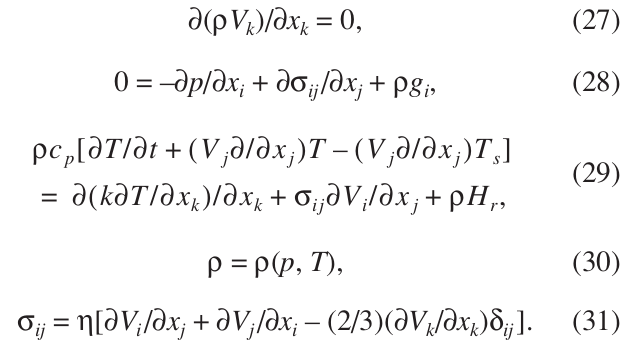
\includegraphics[width=7cm]{images/trub08a}}
\end{center}

}
\end{displayquote}

or, 
\begin{eqnarray}
\vec\nabla\cdot (\rho \vec\upnu) &=& 0 \nn\\
-\vec\nabla p + \vec\nabla \cdot {\bm \sigma} + \rho \vec{g} &=& 0 \nn\\
\rho C_p \left( \frac{\partial T}{\partial t} + \vec\upnu \cdot \vec\nabla (T-T_s)\right) &=&
\vec\nabla \cdot k \vec\nabla T + {\bm \tau}: \vec\nabla \vec\upnu + \rho H_r \nn\\
\rho &=& \rho(p,T) \nn\\
{\bm \tau} &=& \eta \left( \vec\nabla \vec\upnu +\vec\nabla \vec\upnu ^T 
-\frac23 \vec\nabla \cdot \vec\upnu  {\bm 1}\right)
\end{eqnarray}


The author then surprisingly introduces the ``Mean Density Approximation'' (MDA) in Section6.




\begin{displayquote}
{\color{darkgray}

The ALA system of convection equations consists of four equations (27)–(31) 
for the four unknowns $\rho(\vec{r}, t)$, $T(\vec{r}, t)$, 
$p(\vec{r}, t)$, and $\vec\upnu(\vec{r}, t)$. Calculations show that the
buoyancy term in the momentum transfer equation is
most sensitive to lateral density variations. Therefore,
the convection equations can be simplified if we replace
the unknown 3-D distribution of the density $\rho(\vec{r}, t)$ by
a 1d distribution $\rho_r(r, t)$ in all equations except the
buoyancy term. The lateral density variations in the
buoyancy term can be expressed explicitly through the
temperature $T$.

For this purpose, we expand the sought density,
depending on coordinates and time through pressure
and temperature $\rho = \rho(p(\vec{r}, t), T(\vec{r}, t))$, in a Taylor
series in the vicinity of a density distribution depending
only on radius (in spherical coordinates, or on $z$ in Cartesian coordinates) 
$\rho = \rho_r(r)$. Since $\rho_r(r)$ only plays the
role of a reference density distribution, it can be represented by any function of 
radius as close as possible to the sought solution of the convection equations.

The Taylor expansion of the density distribution $\rho(p,T)$ in the vicinity of 
the reference 1d distribution $\rho_r(r,T_0)$ has the form
\[
\rho(p,T) = \rho_r(r,T_0) + 
\left(  \frac{\partial \rho}{\partial T}  \right)_p (T-T_0) + 
\left(  \frac{\partial \rho}{\partial p}  \right)_T (p-p_0) + ...
\]
Here the pressure $p_0$ satisfies the hydrostatic equilibrium condition in the absence of convection
\[
\frac{dp_0}{dr} = - g \rho_r(r),
\]
where r is the moving radius.

Retaining the first terms in the Taylor expansion and
taking into account the definitions of thermal expansion
coefficient 
\[
\alpha = - \frac{1}{\rho} \left(  \frac{\partial \rho}{\partial T}  \right)_p 
\]
and the isothermal bulk modulus $K_T = \rho  \left(  \frac{\partial p}{\partial \rho}  \right)_T$, 
it can be rewritten in the form
\[
\rho(p,T) = \rho_r(r,T_0,p_0) 
\left[
1-\alpha (T-T_0) + \frac{1}{K_T}  (p-p_0) 
\right]
\]


}
\end{displayquote}





\newpage
%%%%%%%%%%%%%%%%%%%%%%%%%%%%%%%%%%%%%%%%%%%%%%%%%%%%%%%%%%%%%%%%%%%%%%%
\subsection{Ciskova et al (2017)}

\begin{center}
\fbox{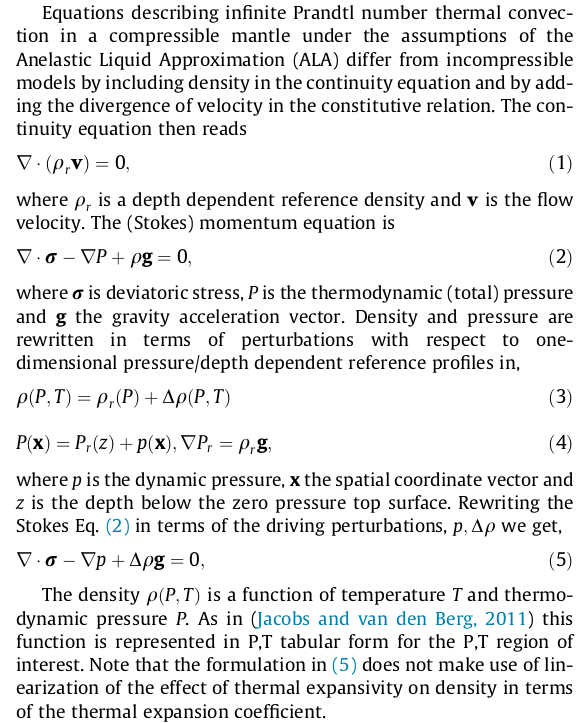
\includegraphics[width=7cm]{images/civj17a}}
\fbox{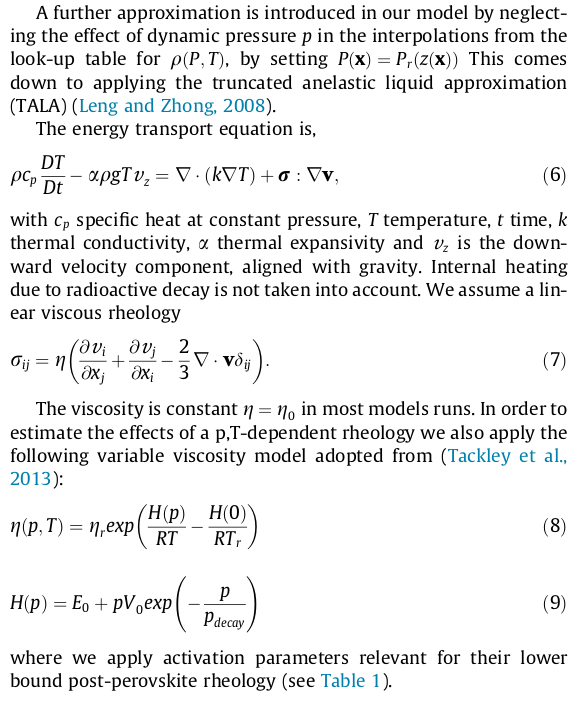
\includegraphics[width=7cm]{images/civj17b}}
\end{center}

{\color{red} finish}


\newpage
%%%%%%%%%%%%%%%%%%%%%%%%%%%%%%%%%%%%%%%%%%%%%%%%%%%%%%%%%%%%%%%%%%%%%%%
\subsection{ASPECT online manual}


\subsection{ALA}
\url{https://aspect-documentation.readthedocs.io/en/latest/user/methods/approximate-equations/ala.html}

COPY!!

\subsection{TALA}
\url{
https://aspect-documentation.readthedocs.io/en/latest/user/methods/approximate-equations/tala.html}

COPY!!











\newpage
\section{Scaling quantities}

Reading the relevant literature from the past 4 decades it looks like the main 
discrepancies/differences seem to come from the quantities used to 
render the main equations dimensionless.

There seems to be two different 'schools':

\begin{itemize}
\item those who normalise the temperature as $T' = \frac{T}{\Delta T}$, for example:
\begin{center}
\fbox{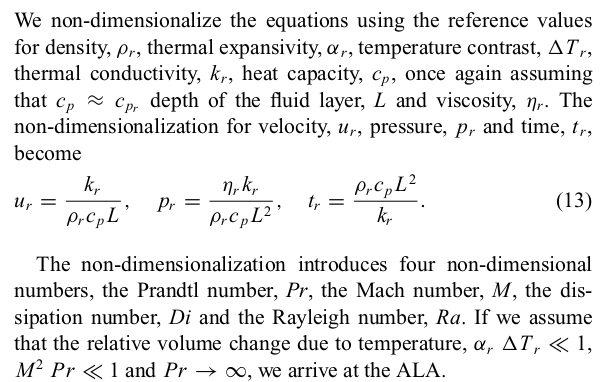
\includegraphics[width=7cm]{images/kilv10}}\cite{kilv10}
\hspace{1cm}
\fbox{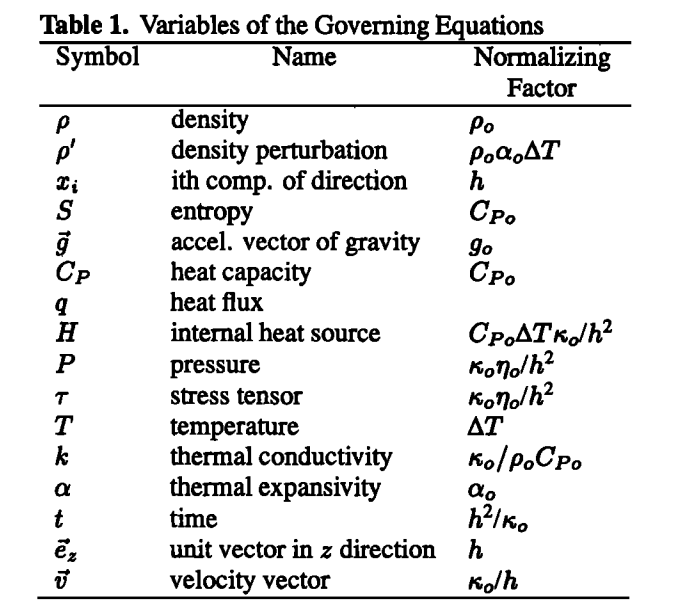
\includegraphics[width=7cm]{images/itki_03}}\cite{itki94}
\end{center}

\begin{center}
\fbox{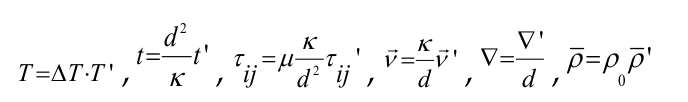
\includegraphics[width=7cm]{images/lee_13}}\cite{lee_13}
\hspace{1cm}
\fbox{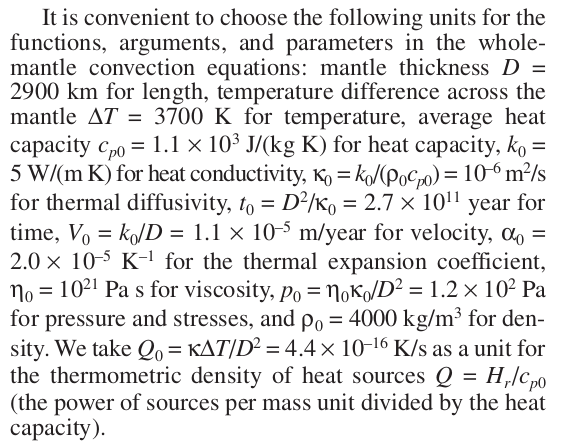
\includegraphics[width=7cm]{images/trub08}}\cite{trub08}
\end{center}


\item those who normalise the temperature as $T' = \frac{T-T_s}{\Delta T}$, where $T_s$
is the surface temperature, for example:
\begin{center}
\fbox{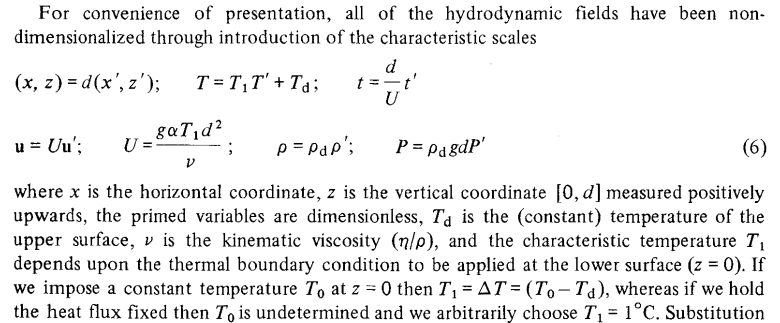
\includegraphics[width=7cm]{images/jape82}}\cite{jape82} \hspace{1cm}
\fbox{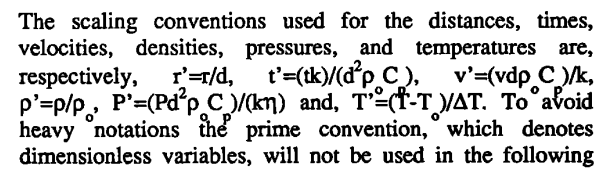
\includegraphics[width=7cm]{images/mayu89}}\cite{mayu89}
\end{center}
\begin{center}
\fbox{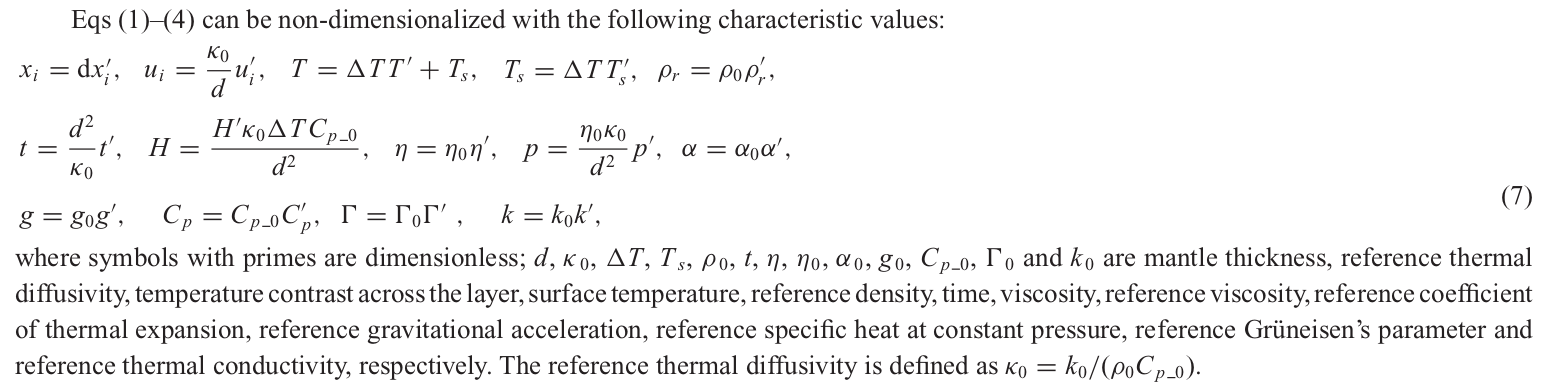
\includegraphics[width=16cm]{images/lezh_04}}\cite{lezh08}
\end{center}

\begin{center}
\fbox{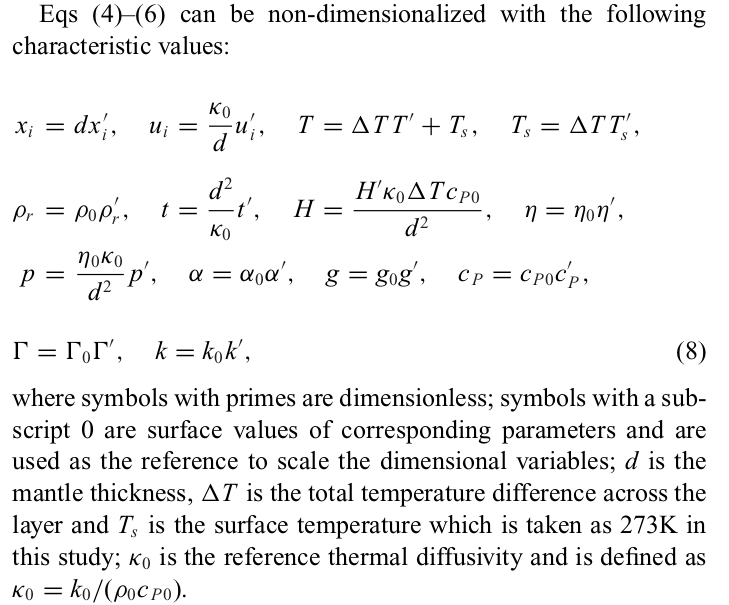
\includegraphics[width=7cm]{images/lizh13}}\cite{lizh13}
\hspace{1cm}
\fbox{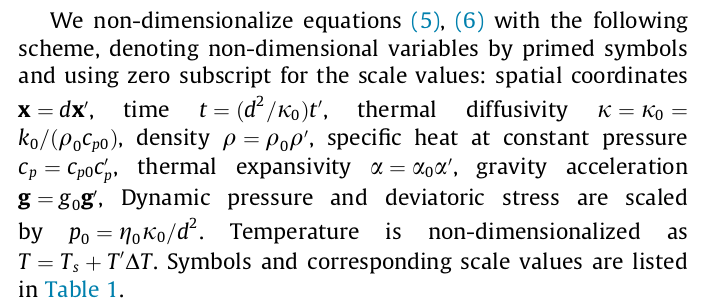
\includegraphics[width=7cm]{images/civj17}}\cite{civj17}
\end{center}


\end{itemize}











\newpage
%%%%%%%%%%%%%%%%%%%%%%%%%%%%%%%%%%%%%%%%%%%%%%%%%%%%%%%%%%%%%%%
\section{Equations of state}

\subsection{Adams-Williamson}

\url{https://en.wikipedia.org/wiki/Adams%E2%80%93Williamson_equation}

check geodynamics syllabus, and do relevant exercises!

\cite{wiad23}

See section 2.2 of \cite{zhyu96b}


%-----------------------------------------
\subsection{Murnaghan}

From Gerya's book II, eq 2.5 (Murnaghan, 1944)
\[
\rho=\rho_0 \left(1 + B_0' \frac{p}{B_0} \right)^{1/B_0'}
\]

%-----------------------------------------
\subsection{Birch-Murnaghan}

From Gerya's book II, eq 2.5 (Birch, 1947)
\[
P(\rho) = \frac{3B_0}{2}
\left[
\left( \frac{\rho}{\rho_0}  \right)^{7/3} - \left( \frac{\rho}{\rho_0}  \right)^{5/3}
\right]
\left\{
1 + \frac34 \left( B_0'-4 \right) \left[ \left(\frac{\rho}{\rho_0}  \right)^{2/3} -1 \right] 
\right\}
\]

where $B_0 = 1/\beta_0$ is the bulk modulus at $p=0$,
$B_0' = (\partial B/\partial p)_{T=cst}$ is the pressure derivative of the bulk modulus at a constant temperature and $\rho_0$ is the density at $p=0$.

%%%%%%%%%%%%%%%%%%%%%%%%%%%%%%%%%%%%%%%%%%%%%%%%%%%%%%%%%%%%%%%%%%%%%%%%%%%%%%%%%%%
\newpage
\section{The final sets of equations to be used in MEEUUW}

\subsection{Thermodynamical quantities}

In \cite{gadb20} we find:
\begin{itemize}
\item the thermal expansivity, describing how much the material
expands due to temperature increases at constant pressure:
\begin{equation}
\alpha = -\frac{1}{\rho} \left(  \frac{\partial \rho}{\partial T} \right)_p
\end{equation}

\item the specific isobaric heat capacity Cp , describing how much
heat is needed to change the temperature of a given material at
constant pressure:
\begin{equation}
C_p= \left(  \frac{\partial q}{\partial T} \right)_p
\end{equation}


\item the isothermal compressibility, describing how much the
material is compressed due to pressure increases at constant temperature:
\begin{equation}
\kappa_T = \frac{1}{\rho}  \left(  \frac{\partial \rho}{\partial p} \right)_T
\end{equation}



\item the isentropic/adiabatic compressibility, describing how
much the material is compressed due to pressure increases at constant entropy:
\begin{equation}
\kappa_S = \frac{1}{\rho}  \left(  \frac{\partial \rho}{\partial p} \right)_S
\end{equation}

\end{itemize}

{\color{red} kappa or K?}

These properties are all second derivatives of the specific thermodynamic potentials 
(specific enthalpy and free energies). Consequently, there are implicit relationships between the parameters (for the derivation, see e.g. section 6.8 of Schubert et al. 2001 {\color{red}check!!}),
which include a relationship between the isothermal and isentropic
compressibilities,
\[
\kappa_S = \kappa_T - \frac{\alpha^2T}{\rho C_p}
\]
and a relationship between heat capacity and the volumetric equation of state:
\[
\left(\frac{\partial C_p}{dp}\right)_T = -T
\left(  \frac{\partial (\alpha/\rho)}{\partial T}\right)_p
\]
These relations also allow us to compute isentropes, which can be
used as reference profiles in some of the compressibility approximations:
\[
\left(
\frac{\partial T}{\partial p} 
\right)_S 
=\frac{\alpha T}{\rho C_p}
\]



\subsection{The full mass, momentum, energy conservation equations}

\subsection{The equations of state}

\subsection{ALA}

\subsection{ALA}

\subsection{ALA}

\subsection{ALA}

















\newpage
%%%%%%%%%%%%%%%%%%%%%%%%%%%%%%%%%%%%%%%%%%%%%%%%%%%%%%%%%%%%%%%
\section{Numerical experiments \& benchmarks}



%--------------------------------------------------------
\subsection{Convection in a box - King et al benchmark}

In this landmark paper, 
``Six 2D Cartesian compressible convection codes
are compared for steady-state constant and temperature-dependent viscosity cases as well
as time-dependent constant viscosity cases. In general we find good agreement between all
codes when comparing average flow characteristics such as Nusselt number and rms velocity.
At Rayleigh numbers near 106 and dissipation numbers between 0 and 2, the results differ
by approximately 1 per cent. Differences in discretization and use of finite volumes versus
finite elements dominate the differences. There is a small systematic difference between the
use of the anelastic liquid approximation (ALA) compared to that of the truncated ALA.''

Although the authors provide multiple tables (in the supplementary material) with all
the results, the dimensionless equations that the authors use are not necessarily 
the ones available to all codes. We prefer to this benchmark the one of the next section, 
which explores the same parameter space, but relying on more standard equations.

%--------------------------------------------------------
\subsection{Convection in a box - Lee 2013}

In a publication published in Korean, Lee carries out the same benchmark
(convection in a box, with BA, EBA, TALA, ALA, for a range of Rayleigh
and dissipation numbers) but with one major difference: the model 
is run with 'real' values  (i.e. not dimensionless) and the 
values of all relevant parameters are presented in the following table: 

\begin{center}
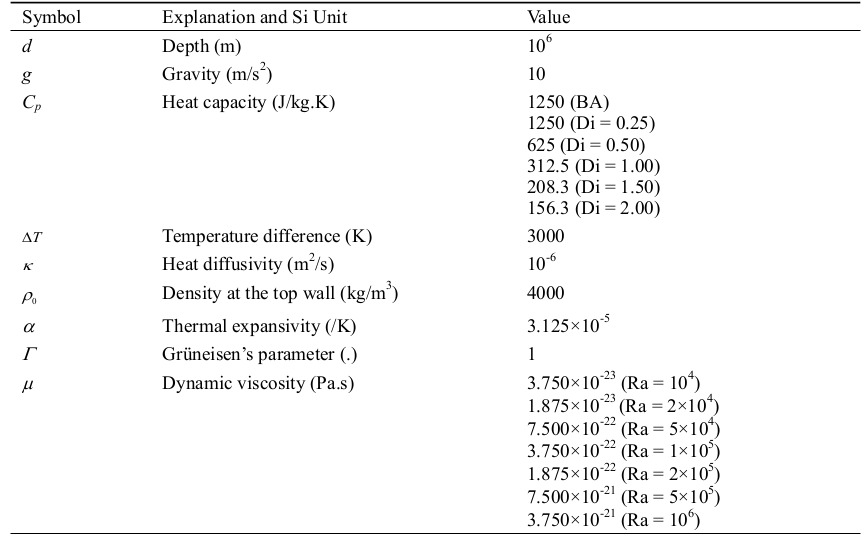
\includegraphics[width=10cm]{images/lee13a}\cite{lee_13}
\end{center}

Also very important is the fact that through the figures of the paper 
we know what the temperature boundary conditions are (only $\Delta T$
matters for BA, but the temperature at the surface also matters for the
other formulations).

The one somewhat puzzling feature of this article is the fact that 
the author does not report on the rms velocity for the whole domain.

The author relies on triangular elements, as well as a bespoke mesh 
with much refinement near the top boundary so as to guarantee 
a higher accuracy of the measurements there (typically, the Nusselt
number).

\begin{center}
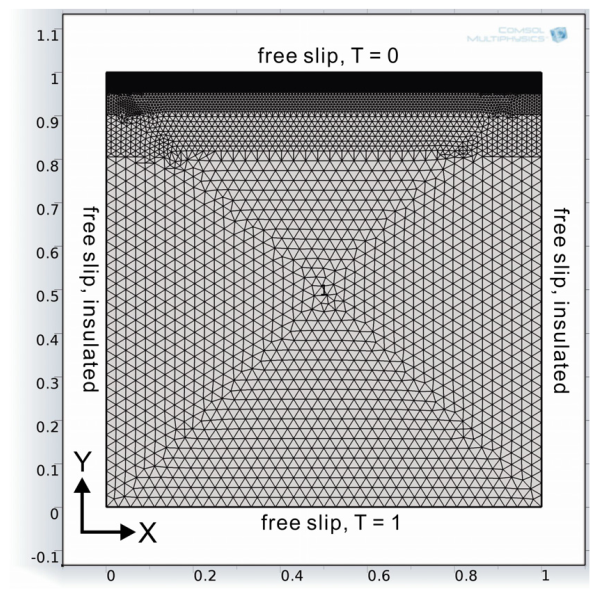
\includegraphics[width=10cm]{images/lee13b}\cite{lee_13}
\end{center}

%--------------------------------------------------------
\subsection{Convection in a box - ASPECT}

In \cite{aaa} the authors carry out the King et al benchmark.

REPORT








\newpage
%%%%%%%%%%%%%%%%%%%%%%%%%%%%%%%%%%%%%%%%%%%%%%%%%%%%%%%%%%%%%%%%%
\section{Conservation of energy }

In what follows we assume for simplicity that the computational domain does not 
deform and that boundary conditions are free-slip on all sides (i.e.
there is not flux of material through the boundaries, i.e. $\vec\upnu\cdot \vec{n}=0$).

In \cite{lezh08} (2008):
\begin{displayquote}
{\color{darkgray}
It has been shown that the total viscous heating and adiabatic heating are exactly 
balanced out for steady-state convection based on energy
balance argument from the energy equation (Turcotte et al. 1974; Hewitt et al. 1975). 
Zhang \& Yuen (1996a) indicated that the total viscous
heating and adiabatic heating should be balanced out at any instant of time based on 
the momentum equation. However, none of these studies
provides an explanation to the imbalance between these two energy terms in previous models 
of compressible mantle convection.
}
\end{displayquote}

%============================================
\subsection{under BA and EBA approximations}

Following \cite{lezh08} (2008), we take the dot product of the momentum 
equation with the velocity $\vec{\upnu}$ and integrate over the whole 
volume\footnote{Check: this is akin to looking at the power, force*velocity,  says Arie}:
\[
\int_V \left[ -\vec\nabla \cdot {\bm \tau}  + \vec{\nabla} p \right] \cdot \vec{\upnu} \; dV  
= \int_V  \rho \vec{g} \cdot \vec{\upnu} \; dV
\]
or, 
\[
-\int_V (\vec\nabla \cdot {\bm \tau})\cdot \vec{\upnu} \; dV 
+\int_V \vec{\nabla} p \cdot \vec{\upnu} \; dV  
= \int_V  \rho \vec{g} \cdot \vec{\upnu} \; dV
\]
Let us look at each term separately:
\[
-\int_V (\vec\nabla \cdot {\bm \tau})\cdot \vec{\upnu} \; dV 
=-\int_S {\bm \tau} \underbrace{\vec{\upnu}\cdot \vec{n}}_{=0 \; (b.c.)} \; dS 
+ \int_V {\bm \tau}:\vec{\nabla} \vec{\upnu} \; dV 
= \int_V {\bm \tau}:\dot{\bm \varepsilon} \; dV 
= \int_V \Phi \; dV 
\]
which is the volume integral of the shear heating. Then, the next term is
\[
\int_V \vec{\nabla} p \cdot \vec{\upnu} \; dV  =
\int_S p \underbrace{ \vec{\upnu}\cdot \vec{n}}_{=0 \; (b.c.)} \; dS 
- \int_V \underbrace{ \vec{\nabla}\cdot \vec{\upnu}}_{=0 \; (incomp.)} \; p \; dV = 0 
\]
which is then zero in the case of an incompressible flow (true under BA and EBA approximations). 
The third remaining term $\int_V \rho \vec{g} \cdot \vec{\upnu} dV = W$ 
is called the work against gravity $W$. 

Conclusion for an {\it incompressible} fluid: we should have
\begin{equation}
\int_V \Phi \;  dV 
=
\int_V \rho \vec{g} \cdot \vec{v} \;  dV 
\label{ba001}
\end{equation}
This formula is hugely problematic: indeed, the term $\rho$ in the rhs is the full density. We know 
that to the value of $\rho_0$ corresponds a lithostatic pressure gradient $p_L=\rho_0 g y$. In this case one can write $\rho = \rho_0 + \rho'$ and $p=p_L + p'$
so that we also have 
\[
\int_V  \left[ -\nabla \cdot {\bm \tau}  
+ \vec{\nabla} p' \right] \cdot \vec{\upnu} \; dV  
= \int_V  \rho' \vec{g} \cdot \vec{\upnu} \; dV
\]
which will ultimately yields 
\begin{equation}
\int_V \Phi \; dV 
= \int_V \rho' \vec{g} \cdot \vec{\upnu} \; dV 
= \int_V (\rho-\rho_0) \vec{g} \cdot \vec{\upnu} \; dV 
\label{ba002}
\end{equation}
Obviously Eqs.(\ref{ba001}) and (\ref{ba002}) cannot be true at the same time.
The problem comes from the nature of the (E)BA approximation: 
$\rho=\rho_0$ in the mass conservation equation
but it is not constant in the momentum conservation equation, which 
is of course inconsistent. Since the mass 
conservation equation is ${\vec\nabla}\cdot \vec{\upnu}=0$ under 
this approximation then the term 
$\int_V {\vec \nabla} p \cdot \vec{\upnu} \; dV$ is always zero for any 
pressure (full pressure $p$, or overpressure $p-p_L$), 
hence the paradox. This paradox will be lifted when a consistent set 
of equations will be used (compressible formulation).
On a practical note, Eqs.(\ref{ba001}) is not verified by the code, while \eqref{ba002} is.   

In the end:
\begin{equation}
\boxed{
\underbrace{\int_V \Phi \;  dV }_{\lstinline{visc_diss}}
=
\underbrace{\int_V (\rho-\rho_0) \vec{g} \cdot \vec{\upnu} \; dV }_{\lstinline{work_grav}}
}
\label{ba003}
\end{equation}


Note that if the fluid is compressible then we have 


\begin{eqnarray}
\int_V \vec{\nabla} p \cdot \vec{\upnu} \; dV  
&=& \int_S p \underbrace{ \vec{\upnu}\cdot \vec{n}}_{=0 \; (b.c.)} \; dS 
-\int_V \vec{\nabla} \cdot \vec{\upnu} \; p \; dV = 0  \nn\\
&=&  \int_V \frac{1}{\rho} \vec{\upnu} \cdot \vec{\nabla} \rho \; p \; dV = 0  
\end{eqnarray}

{\color{red} ToDo}:see section 3 of \cite{lezh08} (2008) 
where this is carried out with the Adams-Williamson eos.





%%%%%%%%%%%%%%%%%%%%%%%%%%%%%%%%%%%%%
\subsection{generic form}

We start with the Reynolds transport 
theorem\footnote{\url{https://en.wikipedia.org/wiki/Reynolds_transport_theorem}} 
(see also p210 of \cite{malvern}).
Given any scalar quantity $B(\vec{r},t)$ associated with a moving fluid, 
the general form of Reynolds transport theorem says 

\[
\frac{D}{Dt} \int_{V_m(t)} B(\vec{r},t) \; dV 
= \int_{V_m(t)} \left[ \frac{\partial B}{\partial t} + \vec\nabla \cdot( B \vec{\upnu})   \right]  \; dV 
=\int_{V_m(t)}  \frac{\partial B}{\partial t}  dV + \int_S B   \vec{\upnu} \cdot \vec{n} \; dS
\]
where we have used the divergence theorem on the last term.
Here, $D/Dt$ is the material derivative, $\vec\nabla$ 
is the usual gradient, $V_m(t)$ denotes the material volume at time $t$, 
and $\vec\upnu$ denotes the velocity vector.

Let us apply to this to $B=\rho C_p T$ and compute the time 
derivative of the internal energy:
\begin{eqnarray}
\frac{d}{dt} \int_V \rho C_p T \; dV 
&=& \int_V \frac{\partial }{\partial t} (\rho C_p T ) \; dV 
+ \int_S \rho C_p T  \underbrace{ \vec{\upnu}\cdot \vec{n}}_{=0 \; (b.c.)} \; dS 
\end{eqnarray}

Remark: $\rho$ is a mass density in \si{\kg\per\cubic\meter},
$T$ is a temperature in \si{\kelvin} and $C_p$ is in \si{\joule\per\kelvin}.
[wiki] ``Heat capacity or thermal capacity is a physical property of matter, defined as 
the amount of heat that must be supplied to an object to produce a unit change in its 
temperature. The SI unit of heat capacity is joule per kelvin (J/K). 
It quantifies the ability of a material or system to store thermal energy.''

{\color{red} ToDo: make link to thermal energy}

Assuming the heat capacity $C_p$ to be constant in time, We have 
\[
\frac{\partial }{\partial t} (\rho C_p T ) 
= C_p T \frac{\partial \rho}{\partial t} + \rho C_p \frac{\partial T}{\partial t} 
\]
In the end
\begin{eqnarray}
\frac{d}{dt} \int_V \rho C_p T \; dV 
&=& \underbrace{\int_V C_p T \frac{\partial \rho}{\partial t} \; dV}_{I} 
+ \underbrace{\int_V \rho C_p \frac{\partial T}{\partial t} \; dV }_{II}
\end{eqnarray}

In order to expand $I$, the mass conservation equation $\partial_t \rho + \vec\nabla\cdot(\rho \vec\upnu)=0$ will be used, 
while the heat transport equation will be used for $II$:

\begin{eqnarray}
I= \int_V C_p T \frac{\partial \rho}{\partial t} \; dV
&=& -\int_V C_p T {\vec\nabla} \cdot (\rho \vec{\upnu}) \; dV \qquad \text{int by parts} \nn\\
&=& -\int_V C_p T \rho \underbrace{ \vec{\upnu} \cdot \vec{n}}_{=0 \; (b.c.)} \; dS 
+  \int_V \rho C_p  \vec{\nabla}  T \cdot \vec{\upnu} \; dV
\\
II=\int_V \rho C_p \frac{\partial T}{\partial t}  \; dV
&=&  \int_V \left[ -\rho C_p \vec{\upnu}\cdot \vec{\nabla}T 
+{\vec\nabla}\cdot k {\vec\nabla} T + \rho H  + \Phi    
+\alpha T \left( \frac{\partial p}{\partial t}+  \vec\upnu \cdot {\vec\nabla} 
p \right) \right] \;  dV \nn\\ 
&=& 
 \int_V \left[ -\rho C_p \vec{\upnu}\cdot \vec{\nabla}T 
+ \rho H  + \Phi    +\alpha T \left( \frac{\partial p}{\partial t}
+ \vec\upnu \cdot {\vec\nabla} p \right) \right] \; dV 
+ \int_V {\vec\nabla}\cdot k {\vec\nabla} T \; dV \nn\\ 
&=& 
 \int_V \left[ -\rho C_p \vec{\upnu}\cdot {\vec\nabla}T 
+ \rho H  + \Phi    +\alpha T \left( \frac{\partial p}{\partial t}
+ \vec\upnu \cdot \vec{\nabla} p \right) \right] \; dV 
+ \int_S  k \vec{\nabla} T \cdot \vec{n} \;  dS \nn\\ 
&=& 
 \int_V \left[ -\rho C_p \vec{\upnu} \cdot \vec{\nabla}T 
+ \rho H  + \Phi    +\alpha T \left( \frac{\partial p}{\partial t}+  
\vec\upnu  \cdot \vec{\nabla} p \right) \right]  \;  dV 
- \int_S  \vec{q} \cdot \vec{n} \; dS  \nn
\label{ba004}
\end{eqnarray}

We see that the same term involving $\vec\upnu\cdot \vec\nabla T$
is present in $I$ and $II$ so that finally:

\begin{eqnarray}
I+II
&=&\frac{d}{dt} \underbrace{\int_V \rho C_p T dV }_{E_T} \nn\\
&=& 
\int_V \left[  \rho H  + \Phi    +\alpha T \left( \frac{\partial p}{\partial t}
+\vec\upnu \cdot \vec{\nabla} p \right) \right] \; dV 
-\int_S  \vec{q} \cdot \vec{n} \;  dS \\ 
&=& 
\int_V \rho H dV 
+\underbrace{\int_V \Phi  dV}_{{visc diss} \Phi_T }  
+\underbrace{\int_V \alpha T \frac{\partial p}{\partial t}  dV}_{{extra}}
+\underbrace{\int_V \alpha T \vec\upnu  \cdot \vec{\nabla} p  dV}_{{adiab heating} \Upsilon_T} 
- \underbrace{\int_S  \vec{q} \cdot \vec{n}  dS}_{{heatflux boundary}} 
\label{ba005}
\end{eqnarray}

{\bf Remark}:
This was of course needlessly complicated as the term $\partial \rho/\partial t$ is always 
taken to be zero, so that $I=0$ automatically. The mass conservation equation is then 
simply ${\vec\nabla}\cdot (\rho \vec{\upnu})=0$. Then it follows that 
\[
0
= \int_V C_p T {\vec\nabla} \cdot (\rho \vec{\upnu}) dV
=-\int_V C_p T \rho \underbrace{ \vec{\upnu} \cdot \vec{n}}_{=0 \; (b.c.)} dS 
+  \int_V \rho C_p  {\vec\nabla}  T \cdot \vec{\upnu} dV 
=  \int_V \rho C_p  \vec{\nabla}  T \cdot \vec{\upnu} dV 
\]
so that the same term in Eq.(\ref{ba004}) vanishes too, and then 
Eq.~\eqref{ba005} is always valid, although one should be careful 
when computing $E_T$ in the BA and EBA cases as it should use $\rho_0$ and not $\rho$.

In the case of the BA, the adiabatic heating and the viscous dissipation terms are not 
taken into account, so that (in the absence of a heat source $H$) 
we end up with 
\[
\frac{d}{dt} \int_V \rho C_p T \; dV 
= 
+\underbrace{\int_V \alpha T \frac{\partial p}{\partial t}  dV}_{{extra}}
- \underbrace{\int_S  \vec{q} \cdot \vec{n}  dS}_{{heatfluxboundary}} 
\]

In \cite{zhyu96b} (1996) we find confirmation:
\begin{displayquote}
{\color{darkgray}
For infinite Prandtl number, it can be shown
from the momentum equations that at each in-
stant of time the work done by the pressure
gradient is balanced by viscous dissipation (e.g.
Turcotte et al., 1974):
\[
\int D \rho \alpha U_r T dv = \int D Ra^{-1} \eta \Phi dv
\]
where the integration is over the whole volume of
the mantle. This equality is useful for checking
the computational code.}
\end{displayquote}



Note: Arie advises me to measure the total heat flux through the boundaries and normalise it 
by the top heat flux. His experience is that the normalised total heat flux is near zero 
for BA, but a few \% for EBA.

{\bf Question}: does the 'extra' term have a name ?


\subsection{A potentially big problem}

The temperature setup is built as follows: $T_{surf}$ is prescribed at the top, 
$T_{surf}+\Delta T$ is prescribed at the bottom. The initial temperature profile 
is linear between these two values. 
In the case of BA, the actual value of $T_{surf}$ is of no consequence. However, i
for the EBA the full temperature is present in the adiabatic heating term on the 
rhs of the heat transport equation, and the value of $T_{surf}$ will therefore 
influence the solution. This is very problematic as there is no real way 
to arrive at the surface temperature from the King paper. On top of this, 
the density uses a reference temperature $T_0$ which too will influence the solution 
without being present in the controlling $Ra$ and $Di$ numbers!!
In light thereof, it will be very difficult to recover the values of King et al for EBA!
I remember the ASPECT authors struggling with the same issue when attempting to 
replicate the same benchmark. I should dig in the ASPECT cookbooks. 




%%%%%%%%%%%%%%%%%%%%%%%%%%%%%%%%%%%%%%%%%%%%%%%%%%%%%%%%%%%%%%%%%%%%%%%%%%%%%%%
\newpage
\section{Global physical quantities}

We consider the following energy equation:
\[
\rho C_p \left(\frac{\partial T}{\partial t} + \vec \upnu\cdot\vec\nabla T\right)
- \vec\nabla\cdot k\vec\nabla T 
= \rho H + \underbrace{ {\bm \tau} : \vec\nabla \vec\upnu } _{\Phi}
+ \underbrace{\alpha T  \vec\upnu \cdot \vec\nabla p }_{\Upsilon}
\]




%-------------------------------------------------
\subsection{Pointwise viscous dissipation term in the energy equation}

FROM 1416. reconcile !
In many publications the shear hearing is denoted by $\Phi$ and is given by 
$\Phi=\tau_{ij}\partial_j \upnu_i={\bm \tau}:{\vec \nabla}{\vec \upnu}$ where 
${\bm \tau}$ is the deviatoric stress tensor.
In what follows I use the index notation as it makes for easier derivations:
\begin{eqnarray}
\Phi 
&=& \tau_{ij}\partial_j \upnu_i \nonumber\\
&=& 2 \eta \dot{\varepsilon}_{ij}^d\partial_j \upnu_i \nonumber\\
&=& 2 \eta \frac{1}{2}\left( \dot{\varepsilon}_{ij}^d\partial_j \upnu_i + \dot{\varepsilon}_{ji}^d\partial_i u_j \right) \nonumber\\
&=& 2 \eta \frac{1}{2}\left( \dot{\varepsilon}_{ij}^d\partial_j \upnu_i + \dot{\varepsilon}_{ij}^d\partial_i u_j \right) \nonumber\\
&=& 2 \eta  \dot{\varepsilon}_{ij}^d  \frac{1}{2}\left(\partial_j \upnu_i + \partial_i u_j \right) \nonumber\\
&=& 2 \eta  \dot{\varepsilon}_{ij}^d   \dot{\varepsilon}_{ij} \nonumber\\
&=& 2 \eta  \dot{\bm \varepsilon}^d :  \dot{\bm \varepsilon} \nonumber\\
&=& 2 \eta  \dot{\bm \varepsilon}^d : \left( \dot{\bm \varepsilon}^d +\frac{1}{3} ({\vec \nabla}\cdot{\vec \upnu}) {\bm 1} \right)\nonumber\\
&=& 2 \eta  \dot{\bm \varepsilon}^d : \dot{\bm \varepsilon}^d 
+ 2 \eta  \dot{\bm \varepsilon}^d : {\bm 1} ({\vec \nabla}\cdot{\vec \upnu}) \nonumber\\ 
&=& 2 \eta  \dot{\bm \varepsilon}^d : \dot{\bm \varepsilon}^d \label{eq:physicsshearheating} 
\end{eqnarray}

This agrees with lee13, aspect manual, but not with kilv10 (
they write tau:grad v = 0.5 tau: eps!)


The shear hearing is denoted by $\Phi$ and is given by 
$\Phi=\tau_{ij}\partial_j \upnu_i={\bm \tau}:{\vec \nabla}{\vec \upnu}$ where 
${\bm \tau}=2\eta \dot{\bm \varepsilon}^d$ is the deviatoric stress tensor.
Using the fact that the deviatoric stress tensor is symmetric, this can be rewritten
\[
\Phi = {\bm \tau}:{\vec \nabla}{\vec \upnu} 
= \frac{1}{2}  \left( {\bm \tau}:{\vec \nabla}{\vec \upnu} + {\bm \tau}^T:{\vec \nabla}{\vec \upnu}^T \right)
= \frac{1}{2}  \left( {\bm \tau}:{\vec \nabla}{\vec \upnu} + {\bm \tau}:{\vec \nabla}{\vec \upnu}^T \right)
=  {\bm \tau}: \frac{1}{2}\left( {\vec \nabla}{\vec \upnu} + {\vec \nabla}{\vec \upnu}^T \right)
=  {\bm \tau}:  \dot{\bm \varepsilon} 
\]

In practice, since both tensors are symmetric we have in 3d:
\[
\Phi = 
\tau_{xx} {\varepsilon}_{xx} +
\tau_{yy} {\varepsilon}_{yy} +
\tau_{zz} {\varepsilon}_{zz} +
2\tau_{xy} {\varepsilon}_{xy} +
2\tau_{xz} {\varepsilon}_{xz} +
2\tau_{yz} {\varepsilon}_{yz} 
\]

Let us turn to the plane strain case.
We start from the 3d strain rate tensor 
\[
\dot{\bm \varepsilon}(\vec\upnu) = 
\left(
\begin{array}{ccc}
\dot{\varepsilon}_{xx} & \dot{\varepsilon}_{xy} & \dot{\varepsilon}_{xz} \\
\dot{\varepsilon}_{yx} & \dot{\varepsilon}_{yy} & \dot{\varepsilon}_{yz} \\
\dot{\varepsilon}_{zx} & \dot{\varepsilon}_{zy} & \dot{\varepsilon}_{zz} 
\end{array}
\right)
\]

The plane strain assumption is such that the problem at hand is assumed to be  
infinite in a given direction. In the case of computational geodynamics, most 2d  
modelling is a vertical section of the crust-lithosphere-mantle
and the underlying implicit assumption is then that the orogen/rift/subduction/etc ... 
is infinite in the direction perpendicular to the screen/paper.  

Let us assume that the deformation takes place in the $x,z$-plane,
so that $v=0$ (velocity in the $y$ direction is zero) and $\partial_y \rightarrow 0$ 
(no change in the $y$ direction).
We then have $\dot{\varepsilon}_{yy}=0$ as well as $\dot{\varepsilon}_{xy}=0$ 
and $\dot{\varepsilon}_{yz}=0$, so that the strain rate tensor is  
\[
\dot{\bm \varepsilon}(\vec\upnu)=
\left( \begin{array}{ccc}
\dot{\varepsilon}_{xx} & 0 & \dot{\varepsilon}_{xz}  \\
0 & 0 & 0 \\
\dot{\varepsilon}_{xz} & 0 & \dot{\varepsilon}_{zz}  
\end{array}\right)
\]
Then 
\[
\Phi = 
\tau_{xx} \dot{\varepsilon}_{xx} +
\tau_{zz} \dot{\varepsilon}_{zz} +
2\tau_{xz} \dot{\varepsilon}_{xz} 
\]
Note that in this case
\[
{\bm \tau}= 2\eta \dot{\bm \varepsilon}^d =
2 \eta 
\left[
\left( \begin{array}{ccc}
\dot{\varepsilon}_{xx} & 0 & \dot{\varepsilon}_{xz}  \\
0 & 0 & 0 \\
\dot{\varepsilon}_{xz} & 0 & \dot{\varepsilon}_{zz}  
\end{array}\right)
-\frac13 ( \dot{\varepsilon}_{xx} + \dot{\varepsilon}_{zz} ) {\bm 1} \right]
=2\eta 
\left( \begin{array}{ccc}
\frac23 \dot{\varepsilon}_{xx} - \frac13 \dot{\varepsilon}_{zz} & 0 & \dot{\varepsilon}_{xz}  \\
0 & -\frac13 ( \dot{\varepsilon}_{xx} + \dot{\varepsilon}_{zz} ) & 0 \\
\dot{\varepsilon}_{xz} & 0 & \frac23 \dot{\varepsilon}_{zz}  - \frac13 \dot{\varepsilon}_{xx} 
\end{array}\right)
\]
and finally
\begin{eqnarray}
\Phi 
&=& \tau_{xx} \dot{\varepsilon}_{xx} +
\tau_{zz} \dot{\varepsilon}_{zz} +
2\tau_{xz} \dot{\varepsilon}_{xz} \nn\\
&=& 
2\eta \left[ 
(\frac23 \dot{\varepsilon}_{xx} - \frac13 \dot{\varepsilon}_{zz} ) \dot{\varepsilon}_{xx} 
+(\frac23 \dot{\varepsilon}_{zz}  - \frac13 \dot{\varepsilon}_{xx} ) \dot{\varepsilon}_{zz}
+2 \dot{\varepsilon}_{xz} ^2 
\right] \nn\\
&=&
2\eta \left[ 
\frac23 \dot{\varepsilon}_{xx}^2 
+\frac23 \dot{\varepsilon}_{zz}^2  
-\frac23 \dot{\varepsilon}_{xx} \dot{\varepsilon}_{zz}
+2 \dot{\varepsilon}_{xz} ^2 
\right] 
\end{eqnarray}


%-----------------------------------------------------------------
\subsection{Pointwise adiabatic heating term in the energy equation}

\[
\Upsilon=\alpha T \frac{Dp}{Dt}
\]
We have $Dp/Dt=\partial p/\partial t + \vec\upnu\cdot\vec\nabla p$ term. 
Often the term $\partial p/\partial t$ is neglected
so that 
\[
\Upsilon = \alpha T \vec\upnu\cdot\vec\nabla p 
\]
If now the pressure is assumed to be mostly hydrostatic in this term then
$\vec\nabla p \simeq \vec\nabla p_L = \rho \vec{g}$ which yields a much simpler formulation:
\[
\Upsilon = \alpha T \vec\upnu\cdot \rho \vec{g}
\]
The same reasoning is presented in 
\url{https://aspect-documentation.readthedocs.io/en/latest/user/methods/basic-equations/adiabatic-heating.html}

Note that if the vertical unit vector $\vec{e}_z$ is pointing upwards then $\vec{g}=-g \vec{e}_z$
so that 
\[
\Upsilon = -\alpha T \upnu_z \rho g_z
\]

{\color{red} minus sign ?!}


%-------------------------------------------------
\subsection{Internal thermal energy}
\[
E_T = \int_V \rho_{(0)} C_p T dV
\]
If BA or EBA are used then the density must be $\rho_0$.


%-------------------------------------------------
\subsection{Gravitational potential energy}
\[
E_G = \int_V \rho g_y (L_y-y) dV
\]

{\color{red} which $\rho$ ?}


%-------------------------------------------------
\subsection{The work done against gravity}

\[
<W>=-\int_V \rho g_y v dV
\]

{\color{red} which $\rho$ ?}



%-------------------------------------------------
\subsection{The kinetic energy}
\[
E_K=\int_V \frac{1}{2}\rho \upnu^2 dV
\]

{\color{red} which $\rho$ ?}


%-------------------------------------------------
\subsection{The total mass}
\[
M_T=\int_V \rho dV 
\]
{\color{red} which $\rho$ ?}

%-------------------------------------------------
\subsection{The average temperature}
\[
<T>=\frac{1}{V} \int_V T dV
\]


%-------------------------------------------------
\subsection{The root mean square velocity}
\[
\upnu_{rms} = \sqrt{\frac{1}{V} \int_V \upnu^2 \; dV }
\]

%-------------------------------------------------
\subsection{The total viscous dissipation}

\[
\Phi_T=\int \Phi dV =\frac{1}{V}\int 2 \eta \dot{\bm \varepsilon}:\dot{\bm \varepsilon} dV 
\]














%%%%%%%%%%%%%%%%%%%%%%%%%%%%%%%%%%%%%%%%%%%%%%%%%%%%%%%%%%%%%%%%%%%%%%%%%%%%%%%
\newpage
\section{FE Implementation}



%-------------------------------------------------
\subsection{In Leng \& Zhong, 2008 \cite{lezh08}}

In this paper we find ...

\[
\begin{pmatrix}
\K & \G + W  \\
\G^T + C & 0
\end{pmatrix}
\cdot
\begin{pmatrix}
\vec{\cal V} \\
\vec{\cal P}
\end{pmatrix}
=
\begin{pmatrix}
\vec{f} \\
\vec{h}
\end{pmatrix}
\]

In contrast with the incompressible Stokes flow problem, we now have two 
additional terms: $C \cdot \vec{\cal V}$ 
and $W\cdot \vec{\cal P}$ from the buoyancy force associated with the dynamic pressure.
Note that for TALA, vector WP is ignored.



\begin{displayquote}
{\color{darkgray}
First, our analysis demonstrates that the Adams-Williamson equation of state is 
energetically consistent for compressible mantle convection with depth-dependent
thermodynamic parameters and material properties. It should be pointed out that 
our analysis does not have any restriction to viscosity and is,
therefore, applicable to variable viscosity structure. \\
Second, our analysis provides a way to analyze energetic consistency in mantle convection.
We think that energetic consistency is an important issue in mantle convection 
that should be carefully analysed when new formulations of
mantle convection or equation of state (e.g. Connolly, 2005) are employed.}
\end{displayquote}






%-----------------------------------------------
\subsection{In Leng \& Zhong, 2011 \cite{lezh11}}

This article presents a compressible code based on AMR.
The authors use the Adams-Williamson equation for density
distribution along vertical direction and obtain $\rho_r(z)=\exp(\gamma (1-z))$
where $z$ is the nondimensional vertical coordinate.


As explained in \cite{lezh11} the discretised mass and momentum conservation
equations yield the following matrix form:
\[
\begin{pmatrix}
\K & \G^T + W  \\
\G + X & -D
\end{pmatrix}
\cdot
\begin{pmatrix}
\vec{\cal V} \\
\vec{\cal P}
\end{pmatrix}
=
\begin{pmatrix}
\vec{f} \\
\vec{h}
\end{pmatrix}
\]
$W$ shows the
effects of dynamic pressure on the buoyancy force,
and $X$ shows the effects of mantle compressibility

Note that in \cite{lezh11} so-called $Q_1\times Q_1$ 
element pairs are used, and these need a stabilisation 
term which in this case is the $D$ block.


%------------------------------------------------
\subsection{In Tan \& Gurnis, 2007 \cite{tagu07}}

In this paper the authors use the TALA formulation.
They end up with:

\[
\begin{pmatrix}
\K & \G^T   \\
\G + C_\beta & 0 
\end{pmatrix}
\cdot
\begin{pmatrix}
\vec{\cal V} \\
\vec{\cal P}
\end{pmatrix}
=
\begin{pmatrix}
\vec{f} \\
\vec{h}
\end{pmatrix}
\]
where $C_\beta$ is a constant matrix corresponding to the second term in 
\[
\vec\nabla\cdot \vec\upnu + \frac{1}{\rho_r} \frac{\partial \rho_r}{\partial z} u_z = 0
\]
where $\rho_r = \rho_r(z)$ is the reference density profile.

The author further state that they have adapted the pressure
correction algorithm \cite{rawa94} and used
the biconjugate gradient stabilized method (BiCGstab) 
to solve the equations iteratively. 
The inverse of the stiffness matrix $\K$ is calculated outside the iteration loop. As a result,
computing each iteration involves only matrix-vector and
vector-vector contractions.

The algorithm is then as follows:
\begin{center}
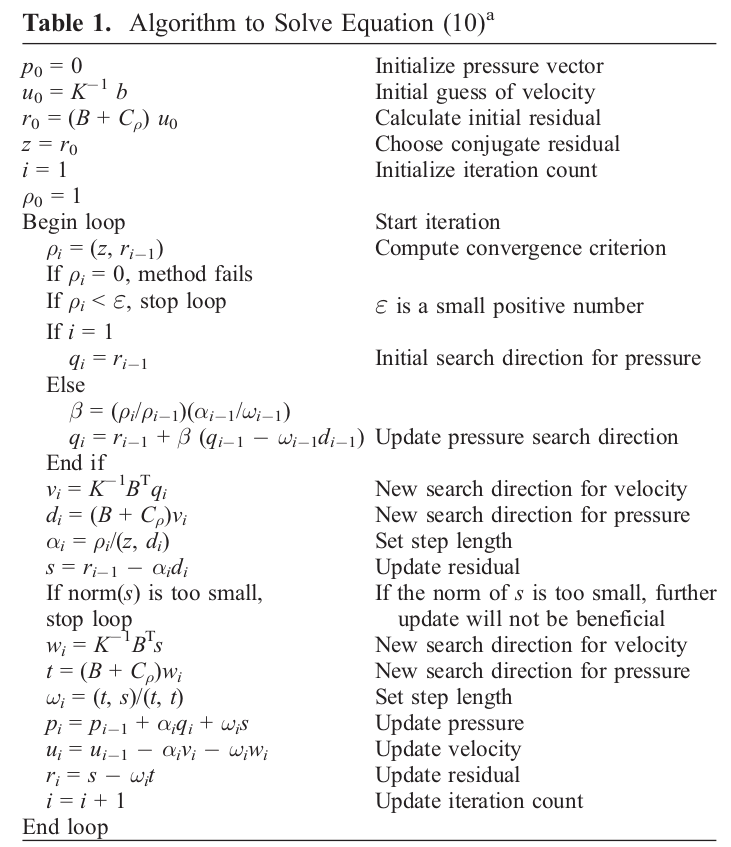
\includegraphics[width=7cm]{images/tagu07}
\end{center}


\subsection{In Heister et al (2017) \cite{hedg17}}




\newpage
\appendix
\section{Lee 2013}
This is obtained by using Google Translate on the original paper written in Korean.


\subsection*{Abstract}

This study conducted a benchmark test using COMSOL Multiphysics, a commercial finite-element-based software widely employed in recent computational geodynamics research. The benchmark involved modeling simple mantle convection while accounting for both incompressible and compressible mantle behavior. The governing equations utilized included the anelastic liquid approximation, truncated anelastic liquid approximation, extended Boussinesq approximation, and Boussinesq approximation; the converged solutions obtained for varying Rayleigh and dissipation numbers were compared. COMSOL Multiphysics proved highly useful for this study due to its user-friendly interface—allowing even non-experts in computational geodynamics to easily construct and run models—and the flexibility it offers for modifying material properties and governing equations. The results align well with established benchmark data. Given its combination of ease of use and accuracy, COMSOL Multiphysics is expected to see widespread application in future computational geodynamics research.


\subsection{Introduction}

If one were to single out the most significant discovery in the history of 20th-century science and engineering, it would be the advent of the computer. 
Since the development of ENIAC (Electronic Numerical Integrator And Computer) (Goldstine, 1972), the first general-purpose computer for ballistic calculations, computer technology has advanced significantly, and currently, computers in almost all fields of science and engineering...
Computers are widely used today. In particular, by enabling massive computational tasks that were previously impossible, computers have driven groundbreaking advancements in the field of numerical analysis; this has made it possible to find numerical solutions for complex partial differential equations that generally lack analytical solutions. Furthermore, the recent emergence of supercomputers—offering vastly superior computational power—has enabled large-scale calculations that were unimaginable just two decades ago.

Consequently, significant efforts have been made since the latter half of the 20th century to solve complex problems in science and engineering using computers and numerical analysis; the geological sciences are no exception to this trend. Even in the 1960s, when computers themselves were a novelty, numerical modeling was employed in pioneering geological research (e.g., McKenzie and Sclater, 1968; Oxburgh and Turcotte, 1968). As computers became more affordable and widely available, research in the geological sciences utilizing computers and numerical analysis expanded rapidly. Within this context, computational geodynamics—a field that uses computers and numerical analysis to study plate motion, deformation, and mantle convection—has established itself as a key area of geological research in the United States, Japan, and advanced European nations. Research in computational geodynamics, covering topics such as mantle convection and subduction processes, continues to be actively conducted today (Sleep, 2006 and references therein; Billen, 2008).


However, computational geodynamics research is an interdisciplinary field that requires knowledge from various related disciplines. First, knowledge of computer programming languages such as Fortran or C is necessary, as well as mathematical knowledge essential for numerical analysis, such as linear algebra and differential equations. Furthermore, because the rheology governing the behavior of plates and the mantle depends on temperature, pressure, and chemical composition, knowledge of geological science and materials science is also required. Due to these characteristics, even developing and utilizing the programs necessary for computational geodynamics research requires significant effort and time; consequently, this acts as an obstacle for geological science majors in acquiring diverse knowledge while conducting research. To overcome this, geological science communities in developed countries [are utilizing specialized computer programmers, applied mathematicians, and geological scientists] with specific characteristics

We have organized a standardized research group and are striving to develop computational geodynamics programs and conduct research using them (e.g., Computational Infrastructure for Geodynamics, www.geodynamic.org and Earthbyte Group, www.earthbyte.org).

Unlike other nations, computational geodynamics research in Korea is still in its infancy; there is a complete lack of comprehensive research programs—such as those found in advanced nations—that utilize specialized research groups to develop and employ relevant software. Therefore, the first priority is to actively introduce geoscientific research utilizing computational geodynamics to the domestic geoscience community and broaden its scope. However, given the critical shortage of researchers in this field, even the initial stage of planning such research—which demands significant time and effort from multiple experts—poses a challenge. Consequently, it is of utmost urgency to foster an environment where not only specialists but also non-specialists can conveniently plan and conduct research, thereby raising awareness and expanding the field's reach.

Given this context, I propose using COMSOL Multiphysics®—a commercial numerical analysis software based on the Finite Element Method (FEM) developed by COMSOL (www.comsol.com)—as an alternative approach for conducting computational geodynamics research. COMSOL Multiphysics is widely utilized across science and engineering fields, enabling the quantitative analysis of complex behaviors in gases, fluids, and solids across one, two, and three dimensions. Notably, it features a Graphical User Interface (GUI) that allows users to easily construct and analyze models using a standard desktop setup with a mouse and keyboard. Furthermore, the software supports parallel computing on supercomputers for computationally intensive tasks, thereby facilitating the execution of highly sophisticated and complex numerical models. In fact, COMSOL Multiphysics has already been frequently employed in studies of plate tectonic processes—such as subduction and mid-ocean ridge dynamics—demonstrating its significant potential for computational geodynamics research (e.g., Carminati and Petricca, 2010; Montési et al., 2011).

Before embarking on full-scale computational geodynamics research using COMSOL Multiphysics—which offers such high potential for application—I intend to conduct the fundamental benchmark tests. While benchmarking of COMSOL Multiphysics for subduction zone modeling has already been performed (van Keken et al., 2008), benchmarks accounting for mantle compressibility and viscous dissipation have not yet been reported. Therefore, in this study, I aimed to compare experimental results obtained using COMSOL Multiphysics with findings from previous studies on 2D incompressible and compressible mantle convection models (King et al., 2010).

%-----------------------------------------------------------------
%-----------------------------------------------------------------
\subsection{Experimental methods}

\subsubsection{2.1: COMSOL Multiphysics}

COMSOL Multiphysics is commercial software based on the finite element method, introduced in 1998 by the Swedish company COMSOL (www.comsol.com), which was founded in 1996; as of December 2012, version 4.3a has been released. It supports the implementation of various 1D, 2D, and 3D numerical models via a graphical user interface, enabling the easy execution of diverse numerical analyses required in science and engineering—ranging from electrical, mechanical, fluid, combustion, and structural analysis to chemical reactions. The program comes with a variety of built-in modeling examples that users can modify to suit their specific needs. Additionally, since material properties can be input as constants or variables, it is possible to construct numerical models with a wide range of material characteristics.

While the modeling examples included in COMSOL Multiphysics are extensive and useful, another significant advantage is the ability for users to freely incorporate ordinary and partial differential equations into their models to suit their specific objectives. This flexibility enables the creation of numerical models tailored to the user's needs. Furthermore, since the built-in differential equations can be modified using simple mathematical notation, anyone with a basic understanding of mathematics can insert or edit these equations.

COMSOL Multiphysics provides post-processing capabilities for results derived from numerical modeling, enabling analysis without the need for external software. For instance, in fluid behavior models, critical parameters such as temperature, pressure, and velocity can be visualized graphically, and specific numerical values can be exported to external files. Furthermore, line, surface, and volume integrals allow for the convenient calculation of various engineering quantities, including fluid and heat flux, enthalpy, and total energy. These features proved particularly useful for comparing the results of this study with those from established benchmarks. More detailed information on COMSOL Multiphysics can be found in the software's manual or in published reference books (e.g., Pryor, 2012).

%-----------------------------------------------------------------
\subsubsection{2.2 Governing Equations for Incompressible and Compressible Mantle Convection}

%-----------------------------------------------------------------
\paragraph{2.2.1 Governing Equations for Mantle Behavior}

Since the establishment of plate tectonics, subduction and mid-ocean ridge spreading can be explained by the global thermochemical circulation occurring between the overriding oceanic plate and the underlying mantle. Mantle behavior, which constitutes the primary component of this thermochemical circulation, can be approximated as the behavior of a highly viscous fluid with temperature- and pressure-dependent viscosity (Schubert et al., 2001). The behavior of such a highly viscous fluid can be described as compressible laminar flow; the governing equations for this flow—partial differential equations representing the conservation of mass, momentum, and energy—are expressed as the continuity, momentum, and energy equations, respectively, as follows (Schubert et al., 2001).

\begin{center}
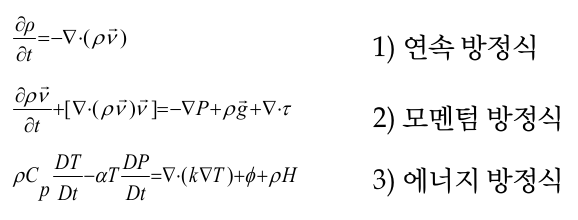
\includegraphics[width=8cm]{images/lee_13/eq_123}
\end{center}

Here, $\rho$ is density (kg/m³), $t$ is time (s), $v$ is the velocity vector (m/s), 
$P$ is pressure (Pa), $g$ is the gravitational acceleration vector (m/s²), 
$\tau$ is the deviatoric stress tensor (Pa), $C_p$ is the isobaric heat capacity (J/kg·K), 
$T$ is temperature (K), $\alpha$ is the thermal expansion coefficient (/K), 
$k$ is thermal conductivity (J/m·K·s), $\phi$ is viscous dissipation per unit volume (J/m³·s), 
and i$H$ is the rate of internal thermal energy generation per unit mass (J/kg·s). 
Viscous dissipation represents the amount of fluid momentum converted into thermal energy i
due to shear stresses arising from fluid motion and is defined as follows.

\begin{center}
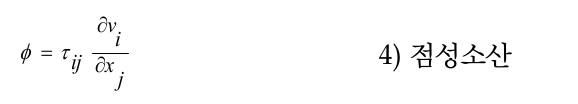
\includegraphics[width=8cm]{images/lee_13/eq_4}
\end{center}

If the mantle were chemically homogeneous and lacked dynamic behavior (such as convection), its density could be expressed solely as a function of temperature and pressure; this is defined as the "reference state." Mantle dynamics—specifically convection—arise from spatial density variations, which are caused by deviations in temperature and pressure from the reference state. Therefore, the actual density of the mantle can be represented by the linear sum of the density defined by the reference state and the density difference resulting from deviations in temperature and pressure. This relationship is expressed mathematically as follows.

\begin{center}
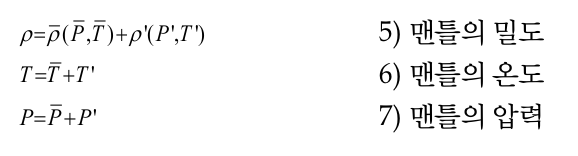
\includegraphics[width=8cm]{images/lee_13/eq_567}
\end{center}

In the above equation, $\rho$, $T$, and $P$ represent the density, temperature, and pressure 
corresponding to the reference state, respectively, while $\rho'$, $T'$, and $P'$ 
represent the density, temperature, and pressure deviating from the reference state. 
In the absence of mantle flow, the reference-state density can be described by the 
Adams-Williamson equation of state (Birch, 1952).


\begin{center}
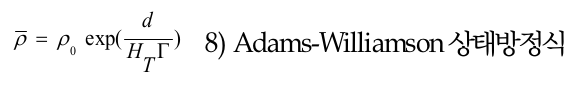
\includegraphics[width=8cm]{images/lee_13/eq_8}
\end{center}

$\rho_0$ is the density of the mantle at the surface, HT is the temperature 
scale height of the compressible fluid, and $\Gamma$ is the Grüneisen parameter; they are defined as follows:

\begin{center}
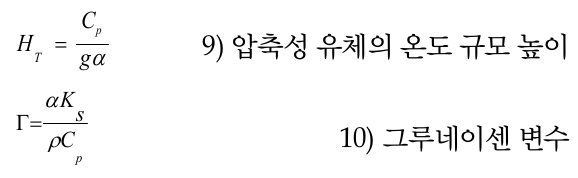
\includegraphics[width=8cm]{images/lee_13/eq_910}
\end{center}

Ks represents the isentropic bulk modulus. By substituting the variables—mantle density, temperature, and pressure—into the governing equation presented above, one can calculate the behavior of the mantle; the following section describes various approximate equations for mantle behavior derived from that governing equation.

%-----------------------------------------------------------------
\paragraph{2.2.2 Anelastic Liquid Approximation (ALA)}

The governing equations for mantle behavior can be simplified because the mantle satisfies the following assumptions (Schubert et al., 2001). First, since the variation in mantle density is negligible compared to the mantle's velocity, the left-hand side of the continuity equation can be approximated as zero. Second, because mantle acceleration is extremely low, the mantle behaves as a fluid with a Mach number effectively equal to zero and a very high Prandtl number (exceeding 10²²). Consequently, the left-hand side of the momentum equation can also be approximated as zero. Applying these two assumptions to the governing equations yields the following set of equations, known as the anelastic liquid approximation (ALA).

\begin{center}
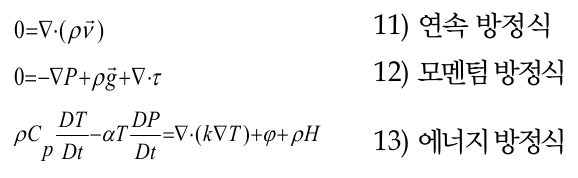
\includegraphics[width=8cm]{images/lee_13/eq_111213}
\end{center}

To efficiently compute the governing equations, non-dimensionalization is performed using the following relevant expressions.

\begin{center}
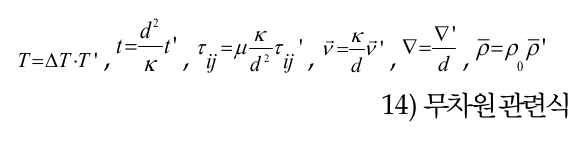
\includegraphics[width=8cm]{images/lee_13/eq_14}
\end{center}

$\Delta T$ is the temperature difference between the top and bottom surfaces of the mantle, 
$d$ is the mantle thickness (m), $\kappa$ is the thermal diffusivity (m²/s), 
$\mu$ is the dynamic viscosity (Pa·s), and $\rho_0$ is the density at the mantle surface (kg/m³). 
After non-dimensionalization, the governing equations-written without the prime symbol for 
convenience-are as follows:

\begin{center}
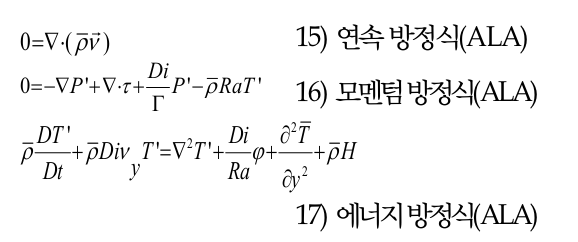
\includegraphics[width=8cm]{images/lee_13/eq_151617}
\end{center}

Non-dimensionalization leads to the derivation of the dissipation number (Di) and the Rayleigh number (Ra), which are defined as follows:

\begin{center}
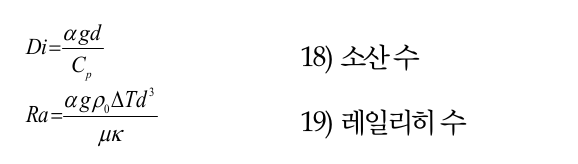
\includegraphics[width=8cm]{images/lee_13/eq_1819}
\end{center}

Since non-dimensionalization also applies to the reference state equation for density, the reference state equation is redefined as follows.

\begin{center}
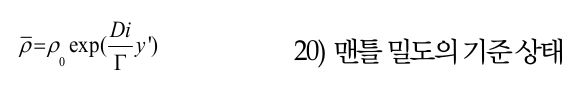
\includegraphics[width=8cm]{images/lee_13/eq_20}
\end{center}

The variable y' represents the mantle depth normalized by the mantle thickness, taking a value of 0 at the surface and 1 at the base. This reference state equation indicates that mantle density increases linearly with depth. The increase in mantle density can be approximated as resulting from adiabatic compression, and the reference state equation for the temperature rise caused by adiabatic compression is derived as follows.

\begin{center}
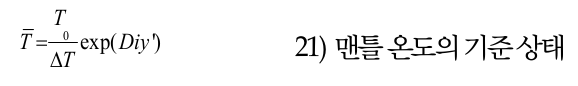
\includegraphics[width=8cm]{images/lee_13/eq_21}
\end{center}

T0 is the temperature at the mantle surface. Like density, this equation indicates that the mantle temperature increases with depth due to adiabatic compression.

%-----------------------------------------------------------------
\paragraph{2.2.3 Truncated Anelastic Liquid Approximation, TALA}


For some numerical modeling packages, difficulties arise in incorporating the dynamic pressure term into the momentum equation due to technical issues (King et al., 2010). In such cases, the dynamic pressure term $\nabla P'$ is omitted from the momentum equation of the anelastic liquid approximation, resulting in the use of the truncated anelastic liquid approximation (TALA). The remaining equations are identical to those of the anelastic liquid approximation.

\begin{center}
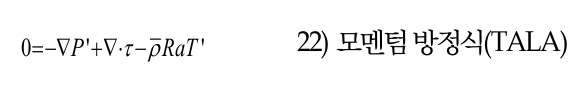
\includegraphics[width=8cm]{images/lee_13/eq_22}
\end{center}

%-----------------------------------------------------------------
\paragraph{2.2.4 (Extended Boussinesq Approximation, EBA)}

The extended Boussinesq approximation (EBA) is an approximation reformulated from the truncated inelastic fluid approximation by assuming the reference-state density to be constant; its governing equations are defined as follows:

\begin{center}
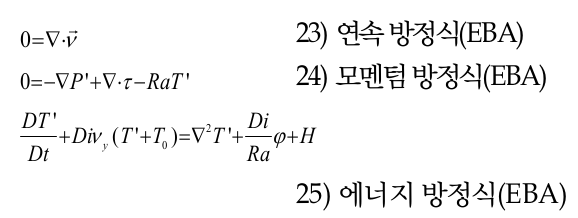
\includegraphics[width=8cm]{images/lee_13/eq_232425}
\end{center}

Vy is the velocity vector in the y-direction. This governing equation is useful for approximating mantle behavior at relatively shallow depths, where the effect of density increase with depth is not significant.



%-----------------------------------------------------------------
\paragraph{2.2.5 (Boussinesq Approximation, BA)}



The Boussinesq Approximation (BA) represents the most simplified governing equations describing the behavior of an incompressible fluid. This approximation is derived by assuming a dissipation number of zero in the energy equation of the extended Boussinesq approximation. Consequently, this assumption is suitable for modeling mantle behavior—where heat generation due to viscous dissipation is expected to be negligible—and is formulated as follows.

insert eq 26

Further details regarding the governing equations described above can be found in previous studies (Jarvis and McKenzie, 1980; Schubert et al., 2001; King et al., 2010). As previously mentioned, the anelastic fluid approximation is the governing equation that most accurately represents mantle behavior. However, due to factors such as technical limitations or the need for model simplification, models employing simplified governing equations—such as the Boussinesq approximation—remain widely used.



%-----------------------------------------------------------------
\paragraph{2.3 Numerical Model}


The derived governing equations and the reference state equations were implemented in COMSOL Multiphysics, and a benchmark study was conducted using two-dimensional finite element modeling. The model used for the benchmark is based on the one presented by King et al. (2010) and is summarized as follows. The model domain is a two-dimensional square; the top and bottom walls are fixed at temperatures of 273 K and 3273 K, respectively, while the side walls are insulated. Additionally, a free-slip condition is assumed for the stress state at all walls, implying that no shear stress acts on the fluid flow. Mantle convection is driven by the temperature difference (3000 K) between the top and bottom walls.
Since the governing equations employed in this study utilize dimensionless quantities, all values used in the modeling are dimensionless. Although mantle viscosity varies significantly depending on temperature, pressure, and composition (Karato and Wu, 1993; Ranalli, 2001), it was assumed to be constant for the sake of the benchmark. Additionally, while internal thermal energy is generated within the mantle through the decay of radioactive isotopes, this factor was neglected for the benchmark (H = 0). The coefficients and constants used in the modeling are listed in Table 1.


In numerical analysis using the finite element method, the accuracy of calculations is significantly affected by the efficiency of mesh formation that constitutes the modeling scope. Generally, using more elements leads to higher accuracy, but this is inefficient because the computation time required for modeling increases significantly as the number of elements increases. COMSOL Multiphysics fundamentally supports the formation of meshes composed of various elements, such as triangles and quadrilaterals.

In this study, a user-controlled mesh was used, and the mesh size was configured to homogeneously form the entire domain using triangular elements suitable for fluid dynamics modeling provided by COMSOL Multiphysics.

Mesh refinement was based on the convection measured at the upper wall of the domain

Mesh refinement is necessary to more accurately measure the Nusselt number—defined as the ratio of convective to conductive heat energy loss at the upper wall of the domain—and the convective velocity at that wall. To achieve this, the upper section of the domain was composed of smaller mesh elements through a three-stage refinement process (Figure 1). The total number of elements resulting from this refinement is 16,065.

For the numerical modeling, the Rayleigh number—a parameter used in previous studies—was varied across the values 
of $10^4$, $2\times 10^4$, $5\times 10^4$, $10^5$, $2\times 10^5$, $5\times 10^5$, and $10^6$. 
Separate experiments were conducted for each Rayleigh number using dissipation numbers of 0.25, 0.50, 1.0, 1.5, and 2.0. When a dissipation number is present, a corresponding reference state equation for mantle temperature—determined by adiabatic compression—exists for each specific dissipation number. For benchmarking purposes in this study, the reference state equation was linearly added to the mantle temperature such that the value at the base of the mantle equaled 3273 K (dimensionless value: 1). In other words, the net temperature difference driving mantle behavior is defined as the total mantle temperature minus the reference state value.


In experiments employing the Boussinesq approximation, terms related to the dissipation number are absent; therefore, the experiments were conducted by varying only the Rayleigh number. A time-dependent solver was used to perform calculations up to a dimensionless time of 1.0, allowing the system to reach a steady state where the results effectively converged. Typically, to initiate mantle convection, COMSOL Multiphysics applies an internal temperature perturbation as an initial condition, which generally results in the formation of a single convection cell within the modeling domain. However, in experiments with high Rayleigh and dissipation numbers, the system may converge to a state with two or more convection cells rather than a single cell. To encourage convergence toward a single convection cell, some experiments utilized the temperature distribution calculated at a lower Rayleigh number as the initial temperature distribution—a method also employed in previous benchmark studies (King et al., 2010).

%------------------------------------
\subsection{Experimental Results}



\subsubsection{3.1 Benchmark}

\paragraph{3.1.1 Anelastic fluid approximation}

First, let us examine the results obtained by varying the Rayleigh number and the dissipation number in a benchmark 
study conducted using the governing equations of the anelastic fluid approximation. Table 2 presents the benchmark 
results, including the Nusselt number (Nu), the maximum velocity at the upper surface of the convecting mantle (Vsurf-max), 
the line integral value of velocity at the upper surface (Vsurf), the average temperature of the entire convection 
cell ($\langle T \rangle$), the thermal energy generated by viscous dissipation within the cell ($\langle \phi \rangle$), 
and the work done by the mantle against gravity ($\langle W \rangle$). Note that all values presented here are 
dimensionless. For details on the calculation methods for these values, please refer to the existing benchmark 
study used for comparison in this research (King et al., 2010).

It was confirmed across all experiments --regardless of the dissipation number-- that the intensity of convection increases 
as the Rayleigh number rises (Figure 2; Table 2). The fact that convective intensity increases with the Rayleigh number 
is already well established (e.g., Blankenbach et al., 1989; King et al., 2010). Figure 2 illustrates the 
temperature distribution within convection cells as the Rayleigh number increases by an order of magnitude --from $10^4$ 
to $10^5$ and then to $10^6$-- while the dissipation number remains fixed at 0.25.


As is already known, it is observed that the thickness of the thermal boundary layers at the top and bottom of 
the convection cells decreases as the Rayleigh number increases; this is reflected in the increase of the Nusselt 
number (Nusselt numbers of 4.410, 9.229, and 14.867 correspond to experimental results obtained with Rayleigh numbers 
of $10^4$, $10^5$, and $10^6$, respectively).
As the intensity of convection increases, the mantle convection velocity rises; this is clearly reflected in the 
increase of both the maximum convection velocity at the upper surface and the line integral value alongside the 
rise in the Rayleigh number (specifically, $V_{surf-max}$ values of 58.065, 252.509, and 749.419 correspond to experiments 
using Rayleigh numbers of $10^4$, $10^5$, and $10^6$, respectively, while $V_{surf}$ values of 38.826, 184.406, 
and 540.730 correspond to the same Rayleigh numbers). Thermal energy due to viscous dissipation ($\langle\phi\rangle$) 
exhibits a linear increase with the Rayleigh number. Similarly, the work done by the mantle against gravity ($\langle W\rangle$) 
shows a linear increase with the Rayleigh number, yielding values nearly identical to those of the thermal energy 
from viscous dissipation. Jarvis and McKenzie (1980) demonstrated that the thermal energy from viscous dissipation and 
the work done by the mantle against gravity exactly cancel each other out; the results of this study confirm that 
these two quantities effectively cancel each other out as well. Furthermore, the mesh resolution test presented 
later in this paper (Section 3.2) indicates that the errors observed in this experiment stem from mesh resolution rather than from any flaws in the governing equations.

Unlike the intensity of convection, which increases with the Rayleigh number, an increase in the dissipation number weakens convective 
intensity (Figure 3). This is clearly demonstrated by the decrease in the benchmark result values as the dissipation number rises. For 
instance, at a dissipation number of 2.0, convective intensity weakens drastically; at a Rayleigh number of $10^4$, 
only very weak convection is observed. A Nusselt number approaching 1 indicates that heat transfer within the mantle 
occurs almost exclusively via conduction rather than convection (at a Nusselt number of 1, mantle convection does not 
occur, and heat transfer relies solely on conduction). This indicates that, unlike the Rayleigh number—which is positively 
correlated with convective intensity—the dissipation number shares an inverse relationship with it.

The results obtained in this experiment were compared with existing benchmark results. With few exceptions, the results showed good agreement with established benchmarks; notably, they aligned very closely—within a relative error of 1\%—with the results from the Virginia Tech (VT) study (King et al., 2010) that utilized the ConMan program (King et al., 1990). Furthermore, for the experiment involving the development of two convection cells, the results showed good agreement with those from the University of Colorado (CU) study that used the Citcom program (Moresi et al., 1996). Although the relative error was observed to increase slightly in experiments with high dissipation numbers, it remained low, generally falling within the 1-4\% range.




\paragraph{3.1.2 Truncated Anelastic Fluid Approximation}
This section summarizes the experimental results obtained using the truncated anelastic approximation governing equations. The truncated anelastic approximation is derived by omitting only the dynamic pressure term from the momentum equation of the standard anelastic approximation. It is generally understood that the dynamic pressure term has a relatively minor influence on fluid behavior compared to other terms (King et al., 2010).

To quantitatively evaluate the impact, results obtained using the governing equations for the truncated anelastic fluid approximation were compared with those obtained using the governing equations for the anelastic fluid approximation. As shown in Figure 4, which plots the relative errors of the comparable results, the discrepancy caused by the dynamic pressure term is relatively large at low Rayleigh numbers. However, the relative error tends to decrease as the Rayleigh number increases. This reduction in relative error—observed in the Nusselt number, thermal energy from viscous dissipation, and work done by the mantle against gravity—is particularly pronounced as the Rayleigh number rises; at Rayleigh numbers of $5 \times 10^5$ or higher, the relative error becomes very small, falling within 2\%. Given that the Rayleigh number of the Earth's mantle is estimated to be around $10^6$ (Schubert et al., 2001), these results indicate that the governing equations for the truncated anelastic fluid approximation can effectively approximate those for the anelastic fluid approximation.

As observed in Table 3, the relative error between the thermal energy generated by viscous dissipation and the work done by the mantle against gravity generally falls within the 0.1–6\% range. When compared with existing experimental results (King et al., 2010), the relative error showed a tendency to increase in experiments with high dissipation numbers but remained low--mostly around 1–4\%--in most cases; significant relative errors of 8–13\% were observed only in experiments using a dissipation number of 2.0 and a low Rayleigh number (e.g., Rayleigh number of $10^4$). 
Overall, however, the experimental results of this study were found to be consistent with those of existing benchmarks.

\paragraph{3.1.3 Extended Boussinesq Approximation}


The extended Boussinesq approximation incorporates the assumption of mantle incompressibility into the truncated anelastic fluid approximation; consequently, the adiabatic temperature profile resulting from adiabatic compression is absent. Due to this assumption, a common approach—used to approximate the actual temperature structure where adiabatic compression occurs—involves conducting experiments based on potential temperature and then linearly adding the adiabatic temperature profile to the results (e.g., Billen and Hirth, 2007; Lee and King, 2011). However, as the primary objective of this study is to benchmark the COMSOL Multiphysics software, no direct comparison regarding these differences was conducted. Therefore, the results obtained using the extended Boussinesq governing equations were not directly compared with the previously described experimental results.

However, the effects of the Rayleigh number and the dissipation number on mantle convection are similar to the experimental results mentioned earlier. The intensity of mantle convection increases as the Rayleigh number rises, whereas it decreases as the dissipation number increases (Table 4). Notably, when the dissipation number is 2.0, mantle convection does not occur in experiments using Rayleigh numbers of $10^4$ and $2 \times 10^4$; this represents a case where the inhibiting effect of viscous dissipation on fluid motion is maximized. It is also noteworthy that, under the extended Boussinesq approximation, the discrepancy between the thermal energy generated by viscous dissipation and the work done by the mantle against gravity is minimal—a trend clearly observed even in experiments employing high Rayleigh and dissipation numbers. The experimental results were compared with existing benchmark data, revealing a relative error of less than 1\% in most cases (results for dissipation numbers of 1.5 and 2.0 
were excluded from the comparison as they were not reported in the existing benchmark studies).


\paragraph{3.1.4 Boussinesq Approximation, BA}

Finally, a benchmark study was conducted using the Boussinesq approximation—the most commonly employed set of governing equations for fluid behavior. As shown in Table 5, the Boussinesq approximation produces the most vigorous mantle convection compared to experiments using other approximate governing equations. Furthermore, in contrast to other approximations—where the flow tends to converge into two or three convection cells or exhibit time-dependent behavior as the Rayleigh number increases—the Boussinesq approximation consistently demonstrated stable convergence to a single convection cell, even at high Rayleigh numbers. These experimental results were compared with existing benchmark data, and all showed a relative error of less than 1\%.

\subsubsection{3.2 Mesh Resolution Test}

In addition to benchmarking the various governing equations introduced above, mesh resolution tests were conducted. Specifically, these tests allowed for the verification of whether the thermal energy generated by viscous dissipation and the work done by the mantle against gravity align accurately within the anelastic fluid approximation framework. While the aforementioned experiments achieved more precise Nusselt number measurements by refining the upper mesh region, the resolution tests focused on varying the element size across three levels without specifically refining the upper mesh section. The experiment using the fewest elements employed the "coarse" mesh setting provided by COMSOL Multiphysics, resulting in a total of 578 elements. The "fine" setting utilized 2,124 elements, while the "extra fine" setting—representing the highest resolution—generated a total of 15,244 elements. To facilitate the mesh resolution tests, the dissipation number was fixed at 0.5, and experiments were conducted by varying only the Rayleigh number.

Table 6 presents the results of the resolution tests conducted for each governing equation. In the experiments using the governing equations based on the anelastic fluid approximation, the Nusselt number is observed to increase as the mesh resolution increases. This occurs because the Nusselt number is calculated using elements closest to the upper surface; consequently, smaller element sizes allow for a more accurate measurement of temperature variations within the thermal boundary layer. In other words, a more accurate Nusselt number is obtained when the element size is smaller.

It was observed that while the Nusselt number is significantly affected by mesh resolution, the differences in other result values are relatively minor. This indicates that modeling results for mantle behavior do not vary substantially even when a relatively small number of elements is used. However, since a tendency for error to increase with the Rayleigh number was observed, a certain level of mesh resolution is essential for accurately calculating mantle behavior at Rayleigh numbers around $10^7$.

In experiments using the governing equations for the anelastic fluid approximation, 
it is observed that the discrepancy between the thermal energy generated by viscous 
dissipation and the work done by the mantle against gravity decreases as mesh resolution 
increases, regardless of the Rayleigh number. Notably, with "extra fine" mesh resolution, 
the relative error between these two calculated values remains within 0.001\% across 
all experiments, indicating that the governing equations for the anelastic fluid approximation 
have been accurately implemented in COMSOL Multiphysics. In contrast, for the truncated 
anelastic fluid approximation—in which the dynamic pressure term is omitted from the momentum 
equation—a nearly constant relative error between the thermal energy from viscous dissipation 
and the work done by the mantle against gravity is observed, irrespective of mesh resolution.


In the case of experiments using the extended Boussinesq approximation governing equations, the observation that the relative error between thermal energy (generated by viscous dissipation) and the work done by the mantle against gravity decreases in proportion to the increase in mesh resolution clearly indicates that higher mesh resolution contributes to improved experimental accuracy. In experiments employing the Boussinesq approximation governing equations, viscous dissipation is absent, and—as in other experiments—increasing the mesh resolution significantly contributes to improving the accuracy of the Nusselt number.

\subsection{Discussion and Conclusion}




Benchmarking results for incompressible and compressible mantle convection, obtained using the finite element-based commercial software COMSOL Multiphysics, showed excellent agreement with existing benchmark results. This demonstrates that COMSOL Multiphysics ensures the accuracy and reliability required for mantle convection modeling while offering advantages such as a graphical user interface and the ease of modifying or inserting material properties and governing equations.

Experiments conducted using various governing equations have demonstrated that mantle compressibility significantly influences the mantle's temperature and convective structure. The estimated dissipation number for the mantle is approximately 0.5, and the Rayleigh number is around $10^7$. Figure 5 presents the converged results of mantle convection calculated for each set of governing equations, assuming a dissipation number of 0.5 and a Rayleigh number of $5 \times 10^5$. As clearly shown in the temperature distributions, experiments accounting for compressibility (Figures 5a and 5b) yield similar results to each other but differ significantly from the experiment conducted under the assumption of incompressibility (Figure 5d). Furthermore, even the experiment utilizing the Extended Boussinesq Approximation—which incorporates the incompressibility assumption into the governing equations of the Anelastic Liquid Approximation (Figure 5c)—shows a marked difference in temperature distribution compared to the experiment based on the incompressibility assumption (Figure 5d). This strongly indicates that, in addition to mantle compressibility, viscous dissipation exerts a significant influence on the mantle's temperature and flow structure.

As this study was conducted to benchmark various programs used for mantle convection research, it did not account for the actual physical properties of the mantle or the phase transformations occurring within it. Viscosity, a key factor influencing actual mantle behavior, can be approximated by diffusion and dislocation creep and is significantly affected by temperature, pressure, grain size, and strain rate (Karato and Wu, 1993; Ranalli, 2001). Therefore, it should be noted that this experiment, which assumes constant viscosity, represents a simplified model of actual mantle behavior. Furthermore, phase transformations (such as olivine to wadsleyite) and phase dissociations (such as ringwoodite to perovskite plus magnesiowüstite)—driven by increasing temperature and pressure—can either enhance or inhibit mantle convection processes like subduction and mantle plumes (King and Ita, 1995; Ita and King, 1998). Consequently, the combined effects of these phase changes and dissociations, along with mantle compressibility and viscous dissipation, would collectively influence mantle temperature and dynamics.

Despite the use of simplified and idealized experimental setups, this study demonstrates that COMSOL Multiphysics offers both convenience and accuracy for modeling mantle convection and subduction, holding significant potential to contribute to future research in this field. Most existing studies have investigated mantle convection and subduction using governing equations that assume mantle incompressibility (such as the Boussinesq approximation)—an approach that remains widely used today. Although some studies have made limited comparisons regarding the effects of compressibility on mantle temperature and behavior (Lee and King, 2009), future research on mantle dynamics and subduction processes must consider mantle compressibility as a crucial modeling factor. The benchmark results presented here are encouraging and serve as a promising starting point for future computational geodynamics research.

Acknowledgments

We would like to express our gratitude to Professors Seung-Seop Kim and Young-Hee Kim for their valuable contributions to improving the quality of this paper. We also thank Professor Young-Kwan Sohn, the Editor-in-Chief, for his assistance. This research was supported by the National Research Foundation of Korea (NRF) with funding from the government (Ministry of Education, Science and Technology) in 2011 (NRF-2011-35B-1-C00043).


\begin{center}
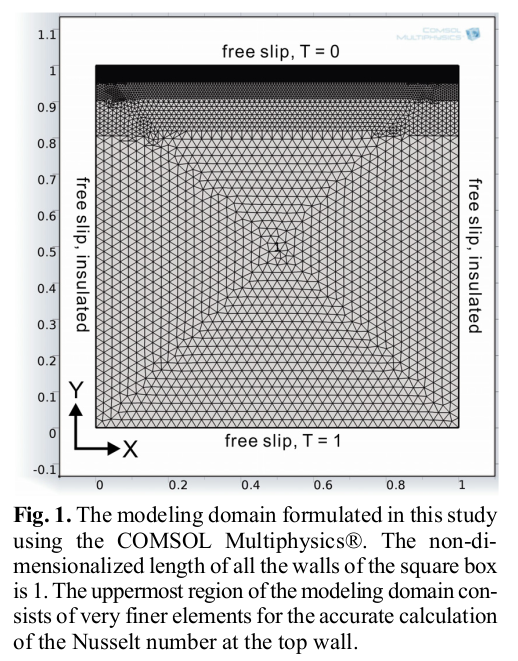
\includegraphics[width=7cm]{images/lee_13/fig1}
\end{center}

\begin{center}
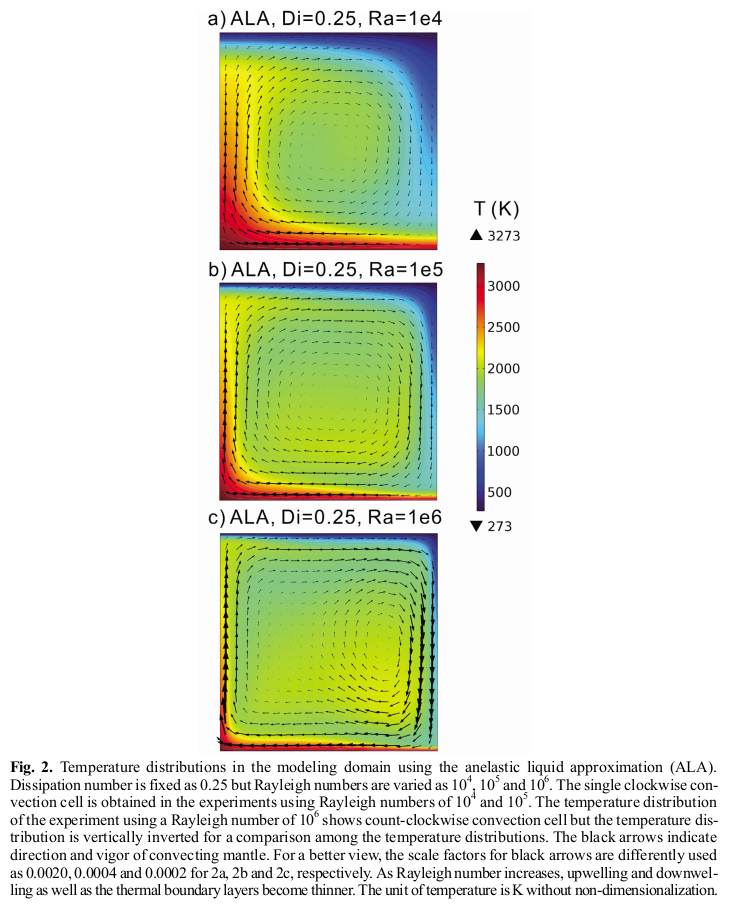
\includegraphics[width=12cm]{images/lee_13/fig2}
\end{center}

\begin{center}
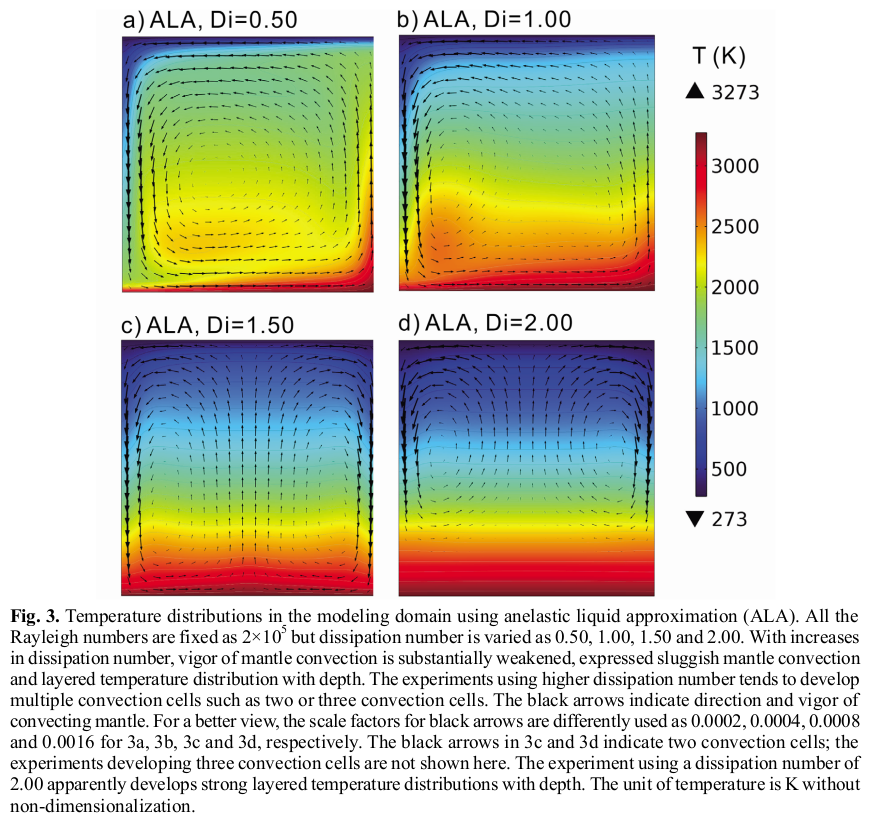
\includegraphics[width=12cm]{images/lee_13/fig3}
\end{center}

\begin{center}
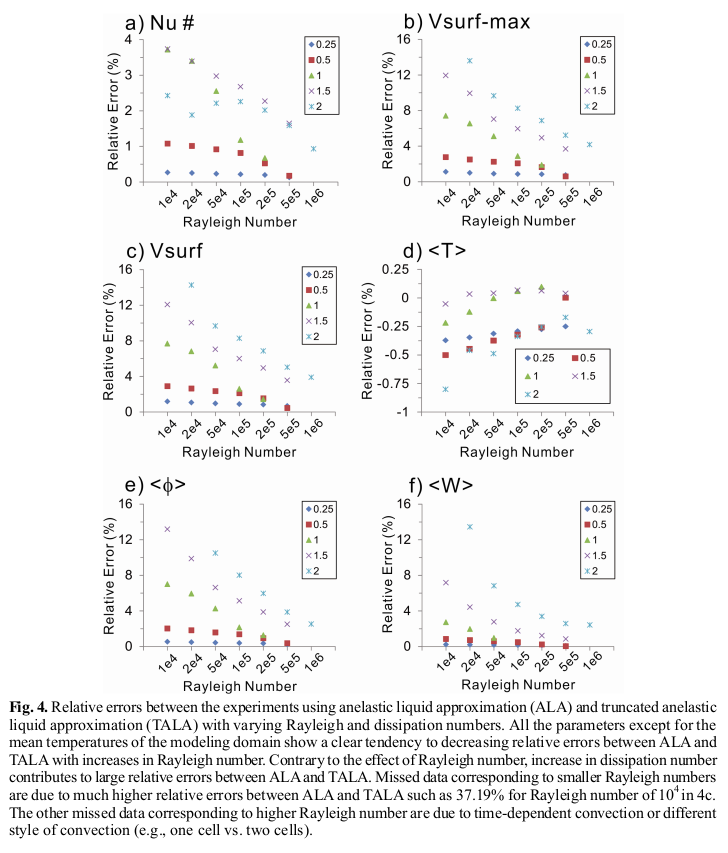
\includegraphics[width=12cm]{images/lee_13/fig4}
\end{center}

\begin{center}
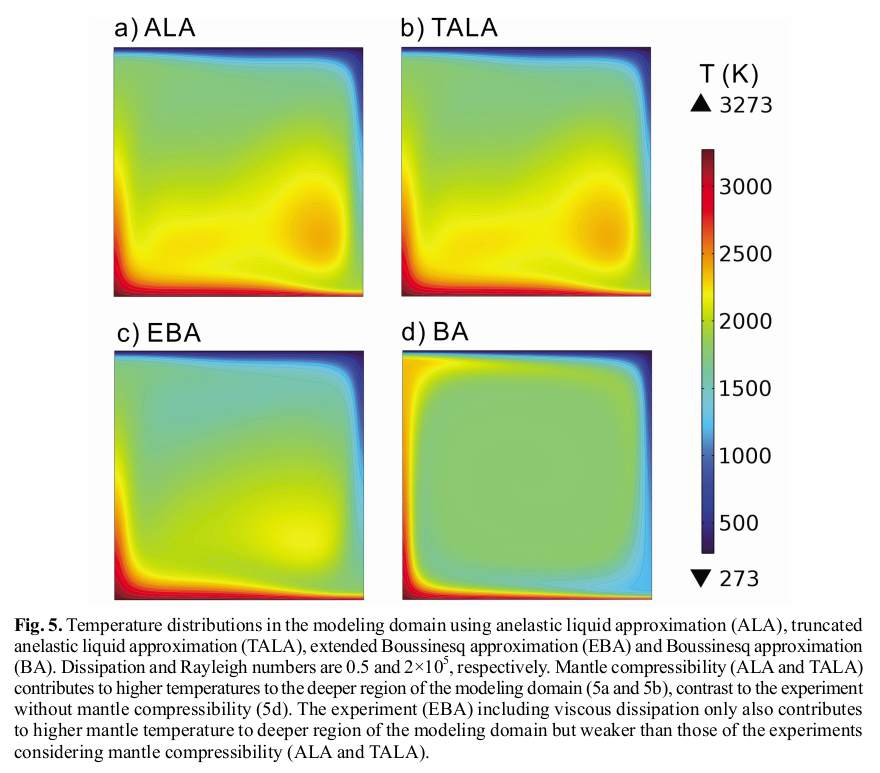
\includegraphics[width=12cm]{images/lee_13/fig5}
\end{center}



\begin{center}
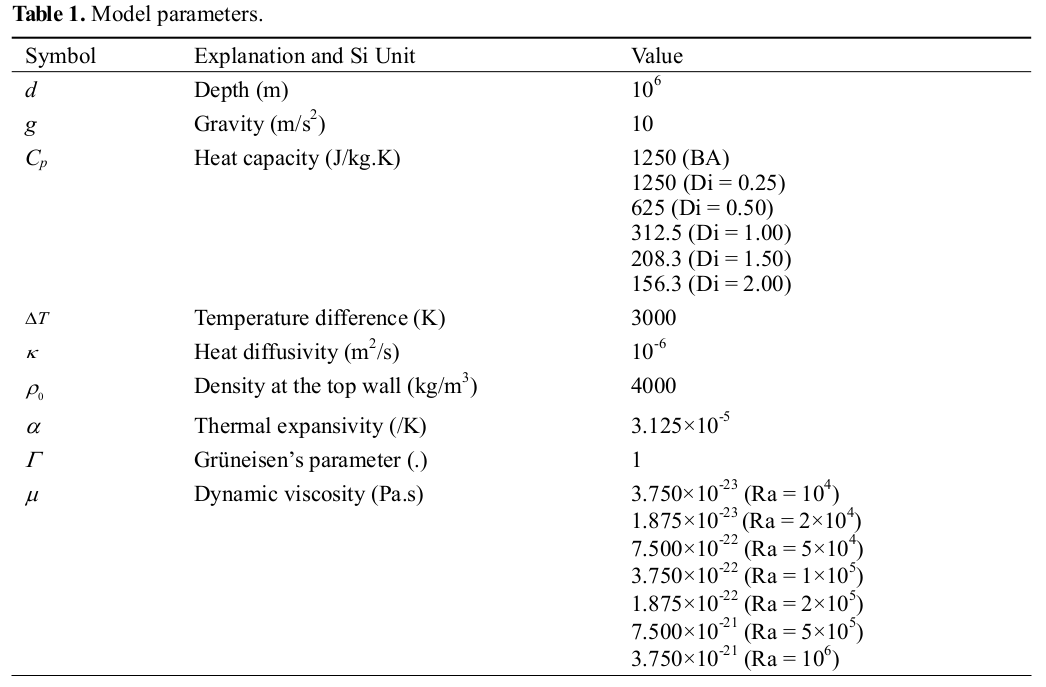
\includegraphics[width=12cm]{images/lee_13/table1}
\end{center}

\begin{center}
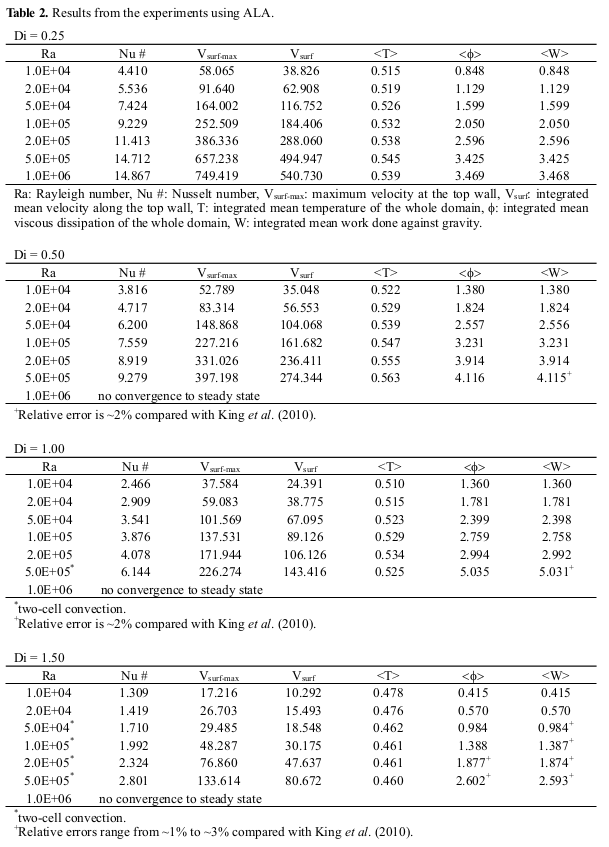
\includegraphics[width=12cm]{images/lee_13/table2a}
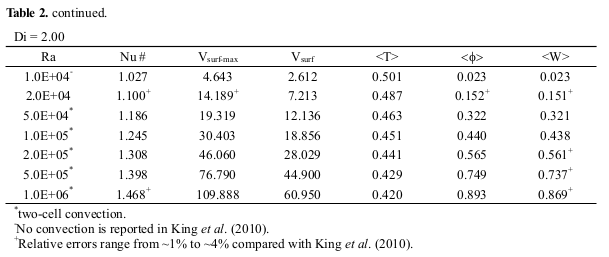
\includegraphics[width=12cm]{images/lee_13/table2b}
\end{center}

\begin{center}
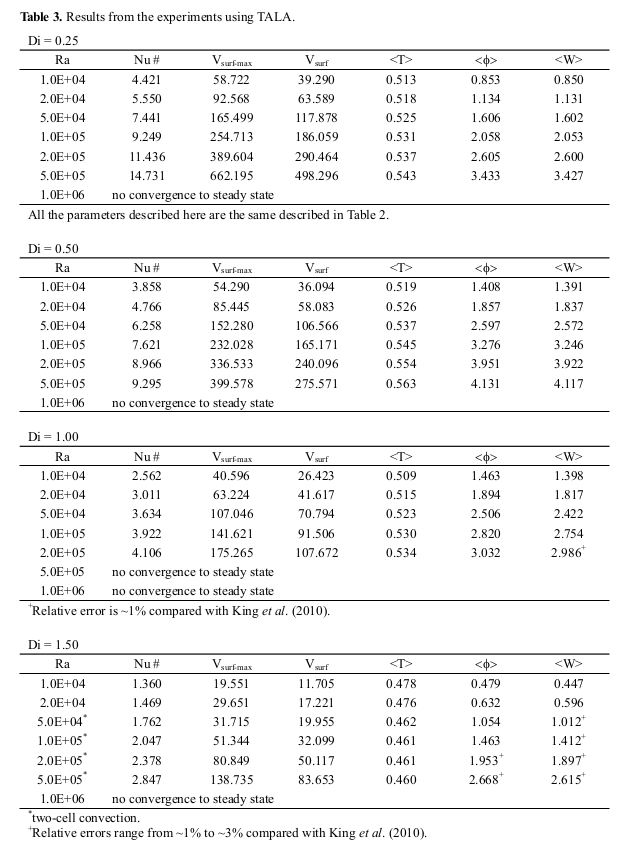
\includegraphics[width=12cm]{images/lee_13/table3a}
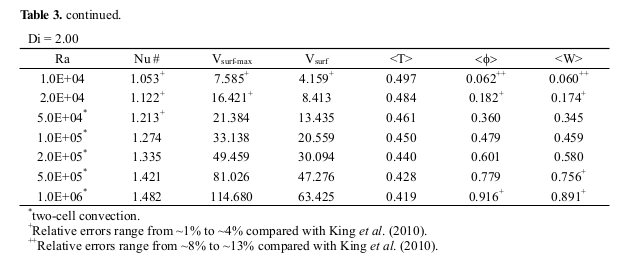
\includegraphics[width=12cm]{images/lee_13/table3b}
\end{center}

\begin{center}
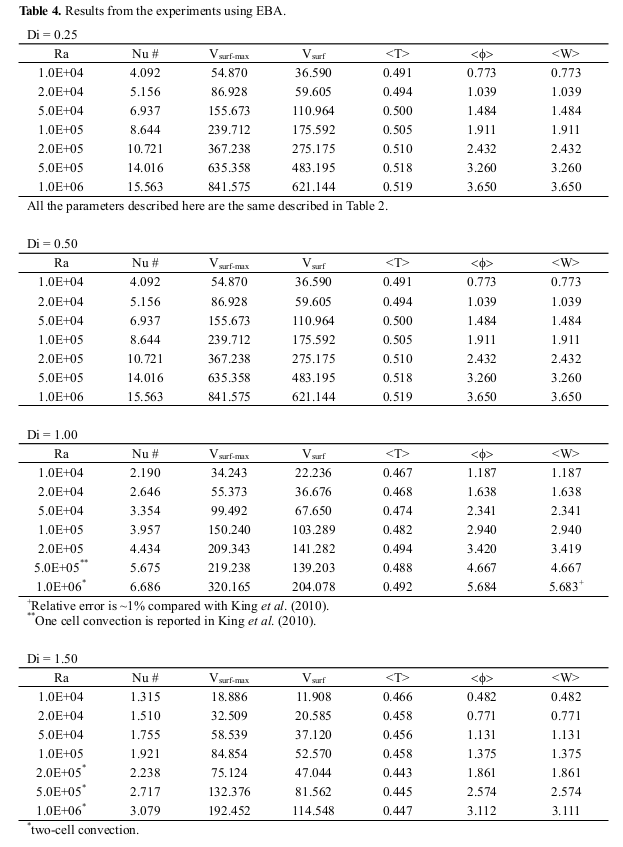
\includegraphics[width=12cm]{images/lee_13/table4a}
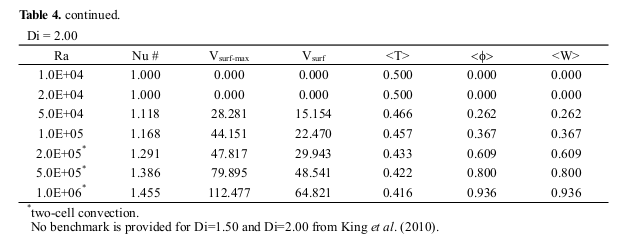
\includegraphics[width=12cm]{images/lee_13/table4b}
\end{center}

\begin{center}
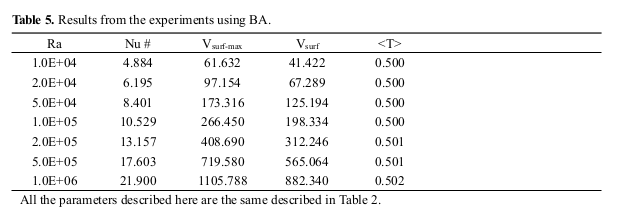
\includegraphics[width=12cm]{images/lee_13/table5}
\end{center}

\begin{center}
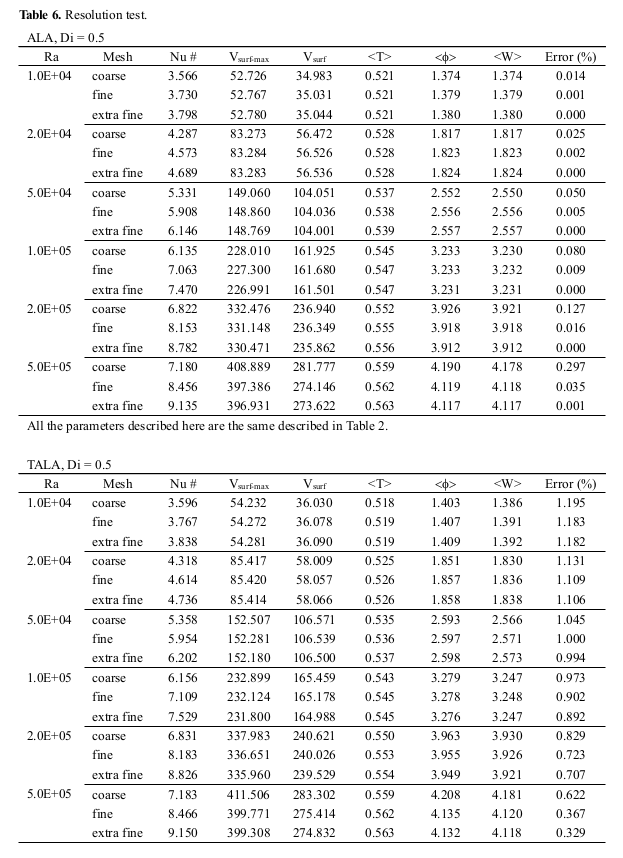
\includegraphics[width=12cm]{images/lee_13/table6a}
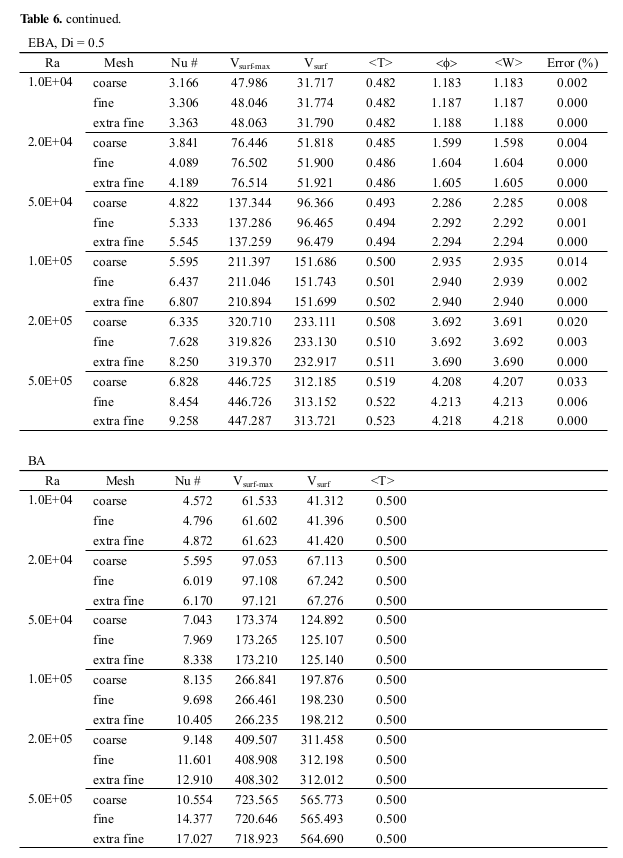
\includegraphics[width=12cm]{images/lee_13/table6b}
\end{center}




























\newpage

\bibliographystyle{apalike}
\bibliography{biblio_lou.bib}

\end{document}


